\section{PIP Input Similarities}
\label{appendix:intprob}

\subsection*{Global Features}

\begin{figure}[h]
  \centering
  \begin{subfigure}[t]{0.32\textwidth}
    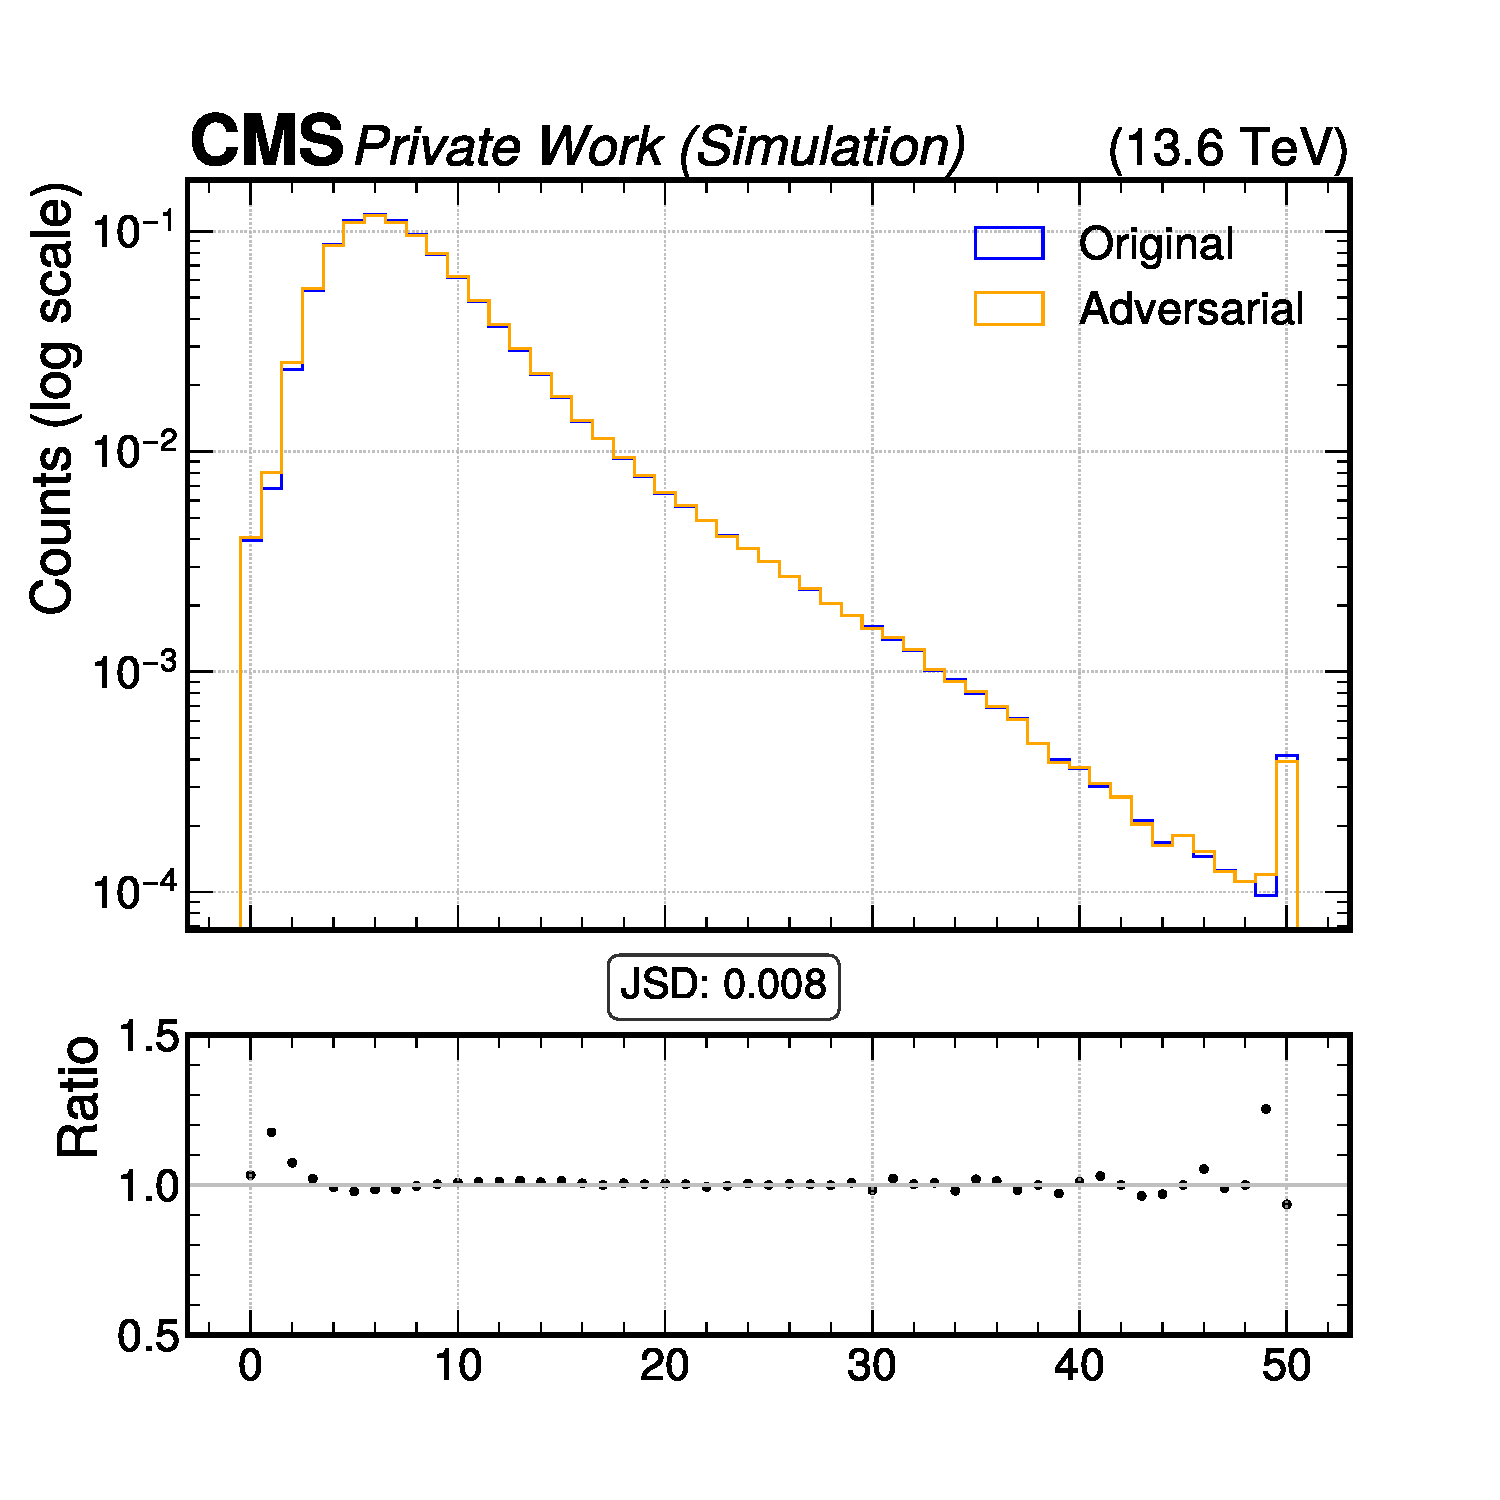
\includegraphics[width=\linewidth]{media/output/features/compare/intprob_1/cmp_global_features_n_Cpfcand.pdf}
    \caption{Input similarity for PIP(1).}
  \end{subfigure}\hfill
  \begin{subfigure}[t]{0.32\textwidth}
    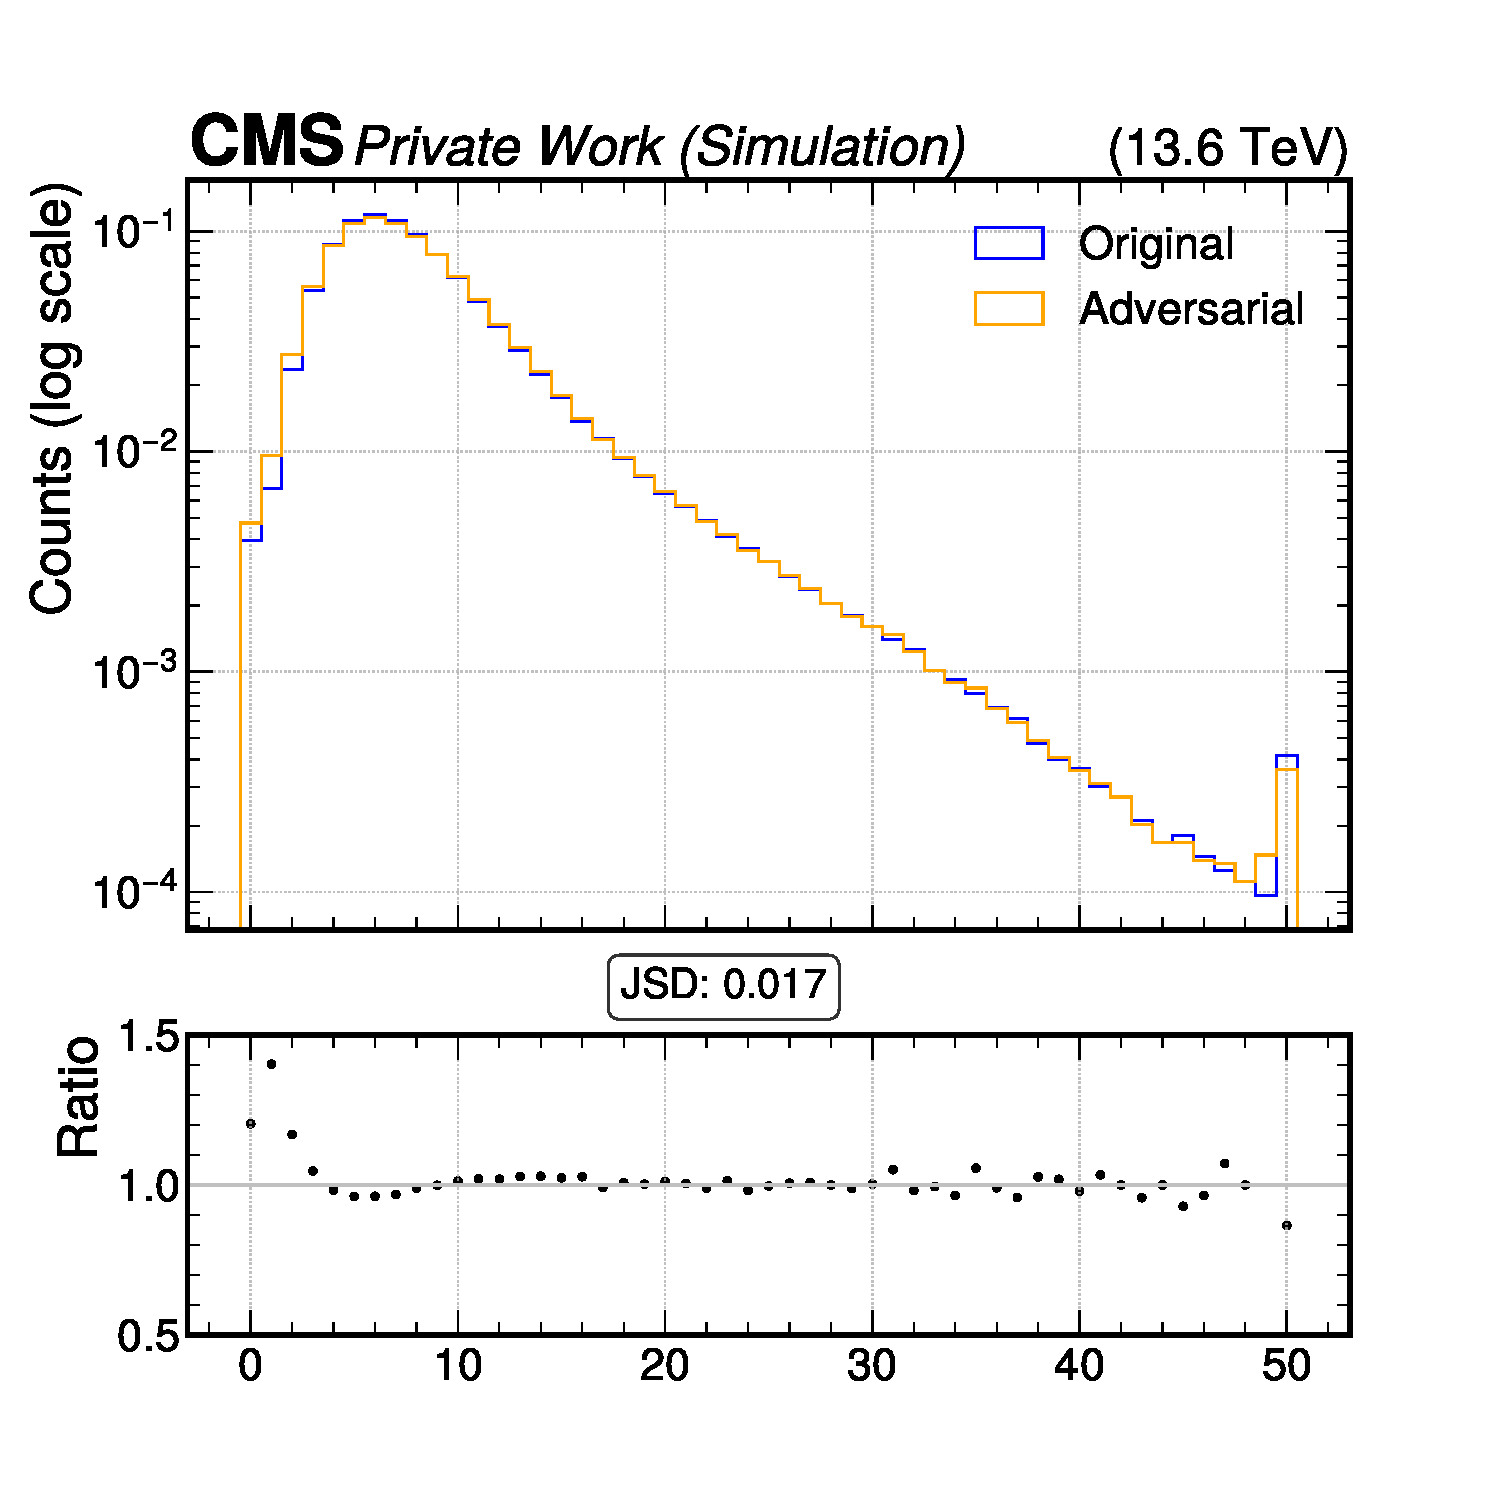
\includegraphics[width=\linewidth]{media/output/features/compare/intprob_2/cmp_global_features_n_Cpfcand.pdf}
    \caption{Input similarity for PIP(2).}
  \end{subfigure}\hfill
  \begin{subfigure}[t]{0.32\textwidth}
    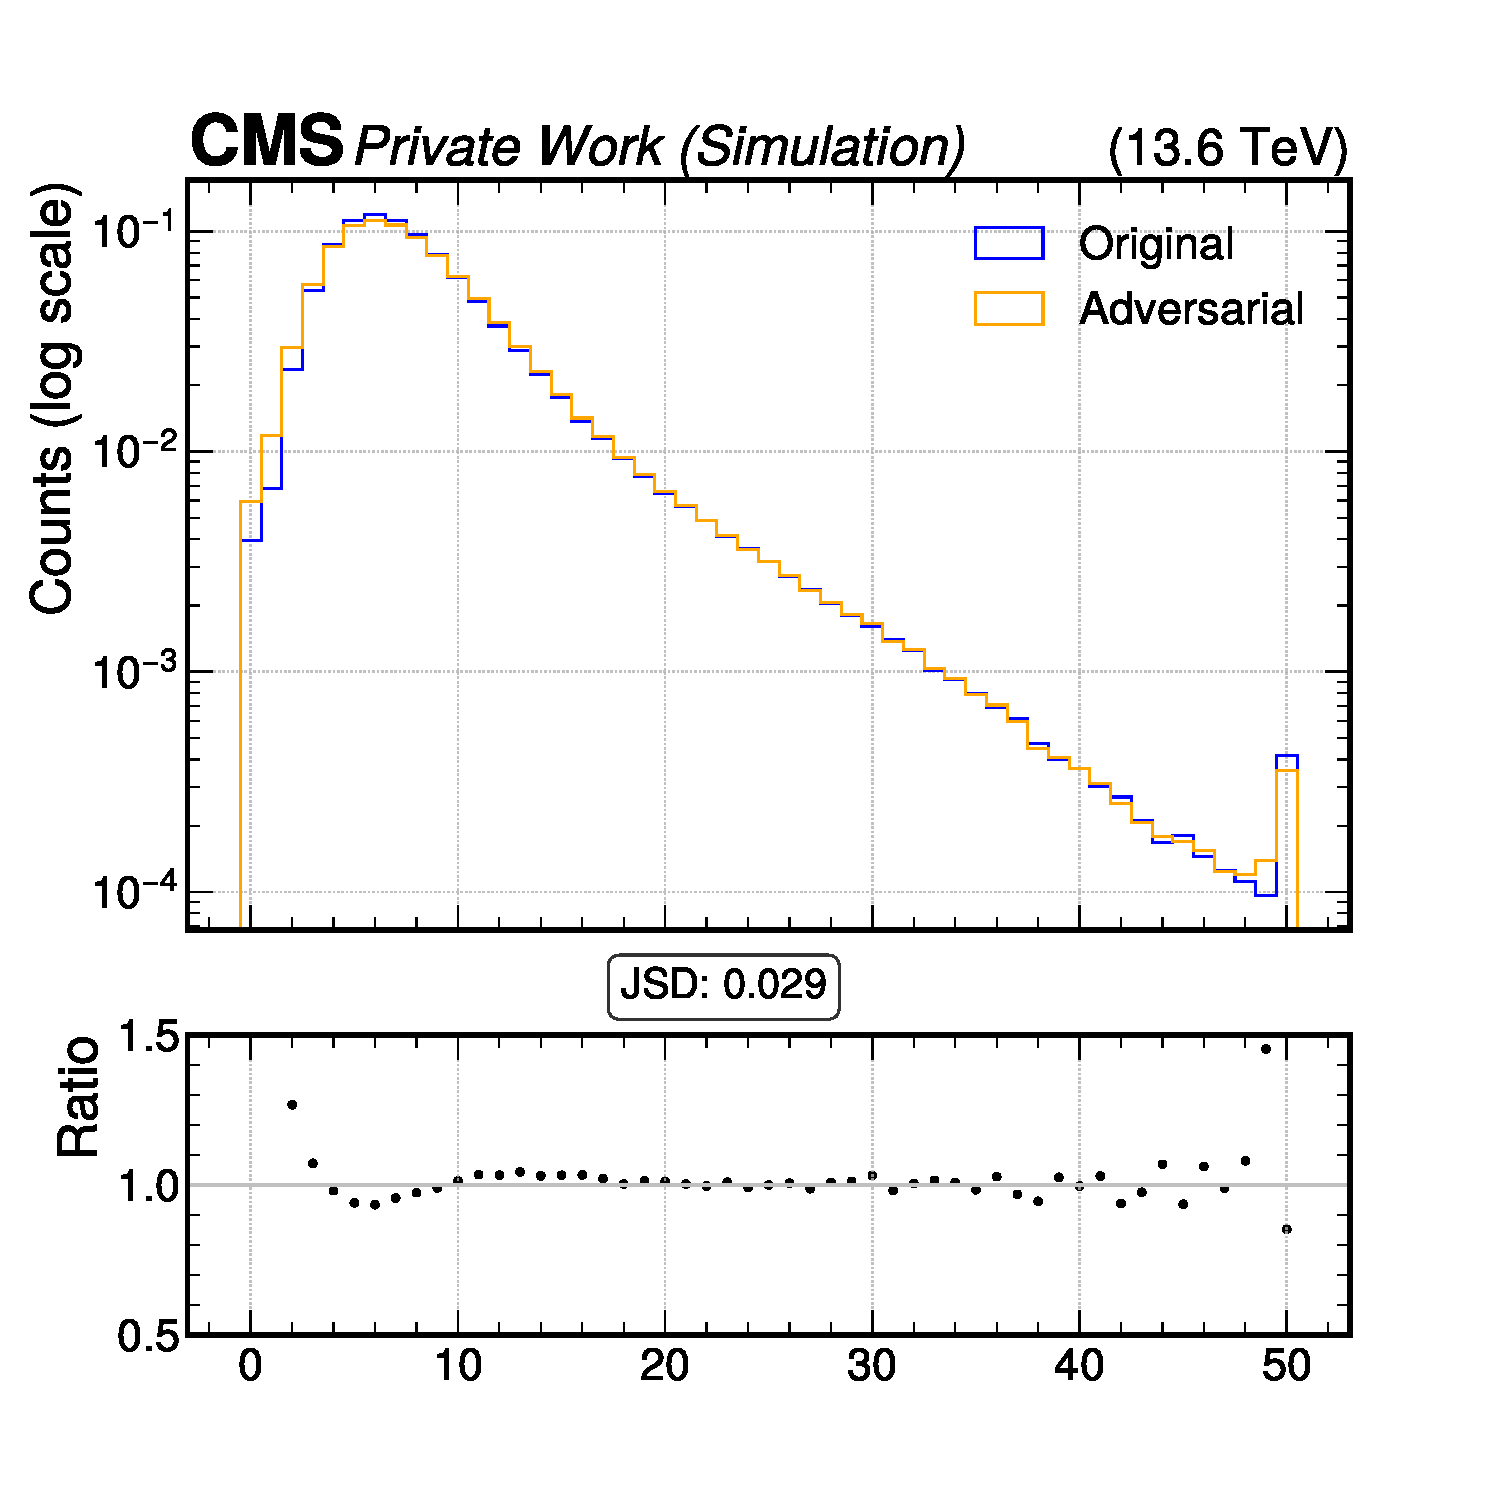
\includegraphics[width=\linewidth]{media/output/features/compare/intprob_3/cmp_global_features_n_Cpfcand.pdf}
    \caption{Input similarity for PIP(3).}
  \end{subfigure}

  \caption{Histogram of \texttt{n\_Cpfcand} for multiple iterations of PIP tested against nominal inputs.}
  \label{fig:intprob_input_n_Cpfcand}
\end{figure}
\begin{figure}[h]
  \centering
  \begin{subfigure}[t]{0.32\textwidth}
    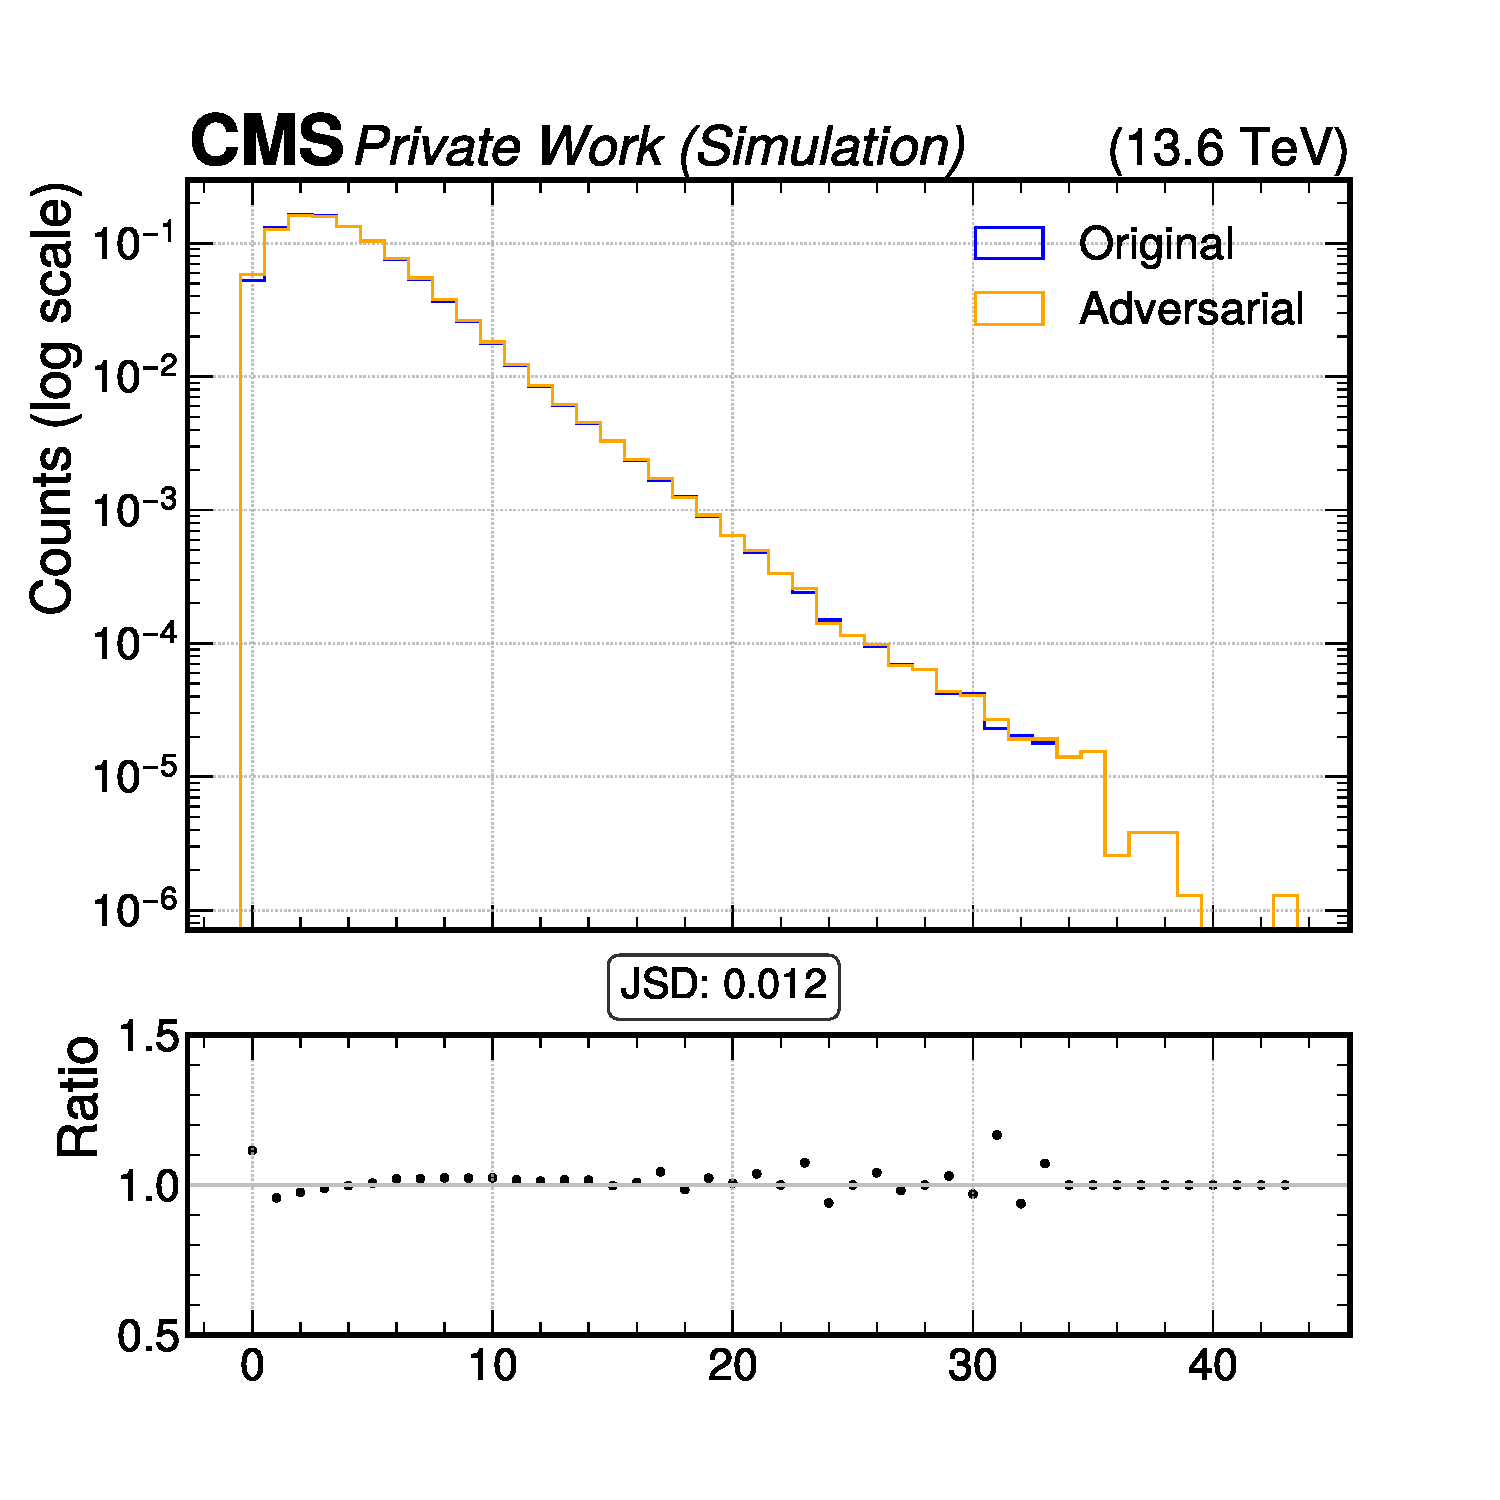
\includegraphics[width=\linewidth]{media/output/features/compare/intprob_1/cmp_global_features_n_Npfcand.pdf}
    \caption{Input similarity for PIP(1).}
  \end{subfigure}\hfill
  \begin{subfigure}[t]{0.32\textwidth}
    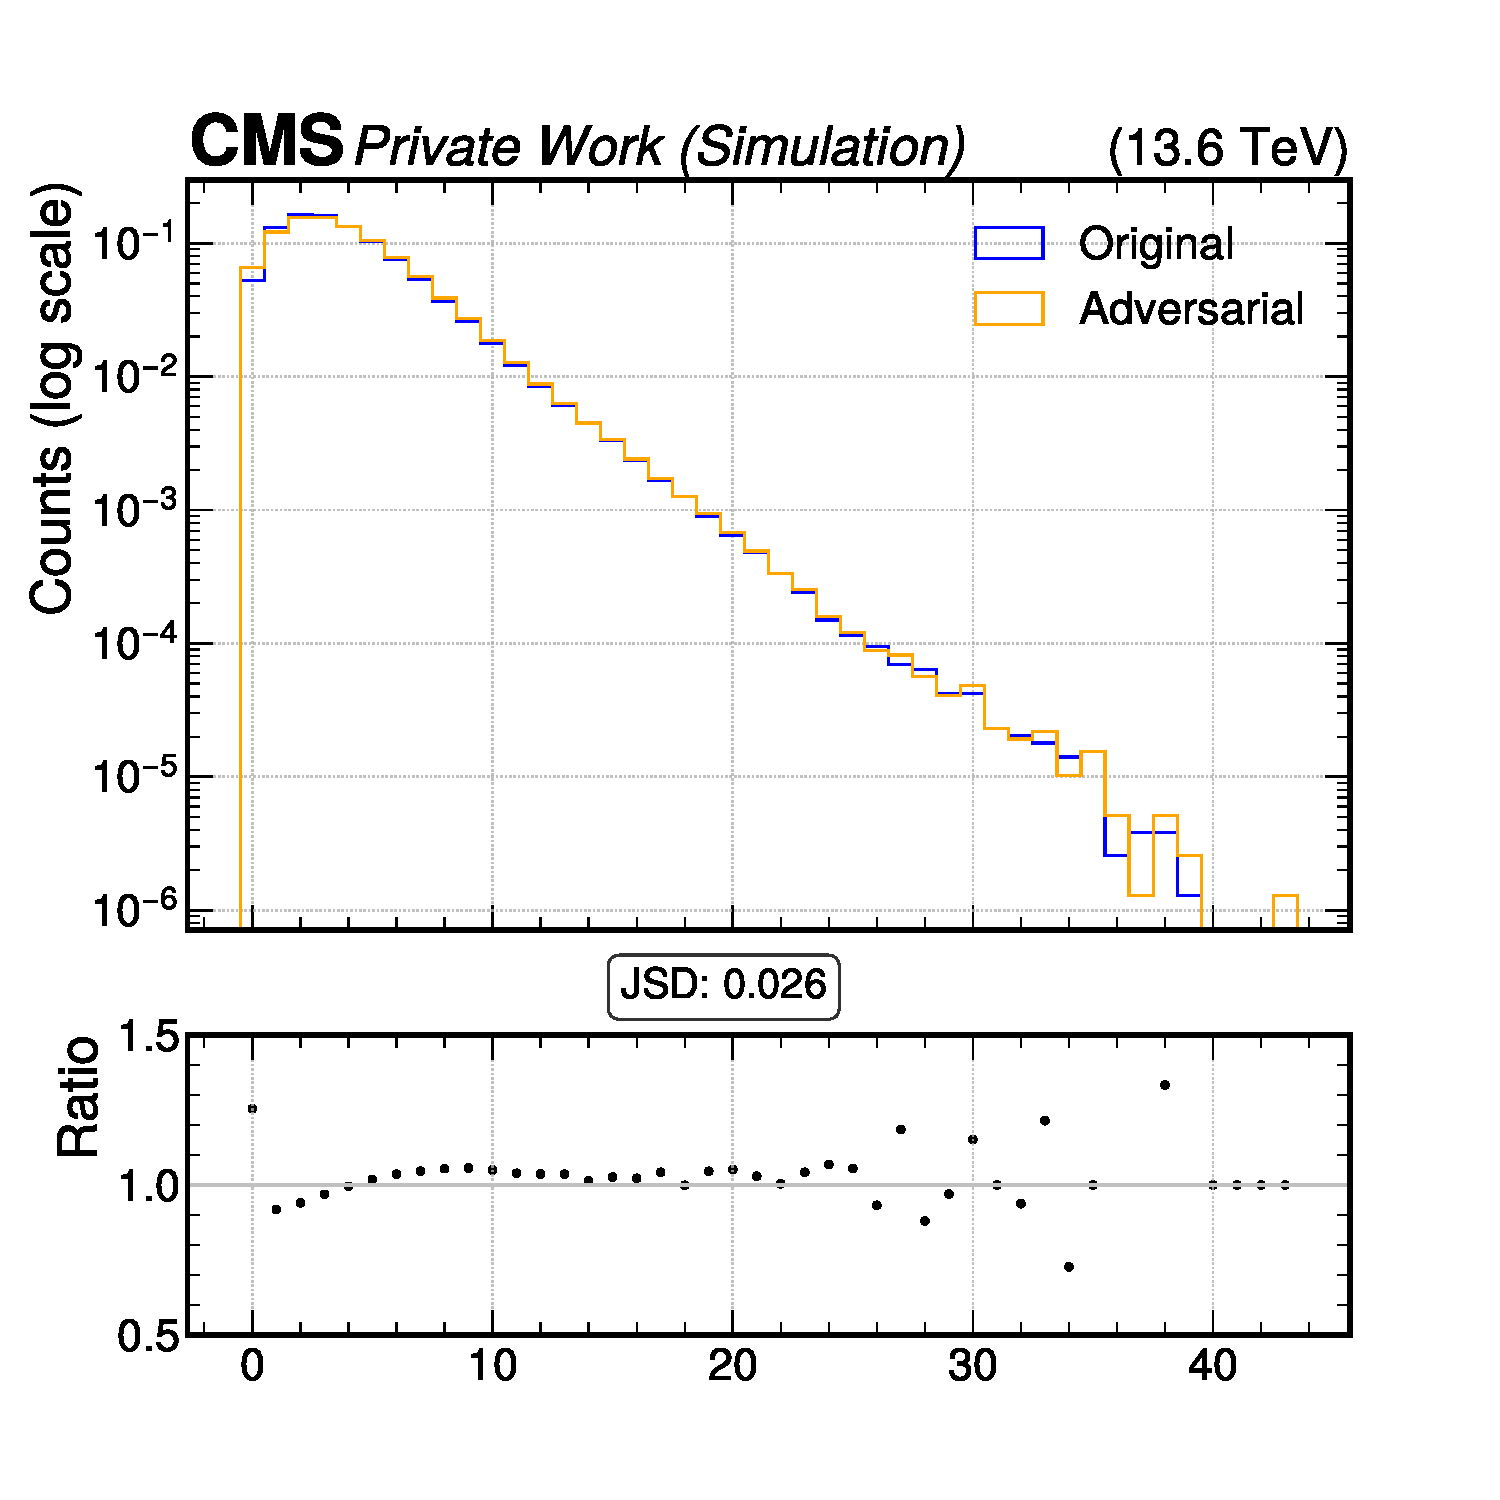
\includegraphics[width=\linewidth]{media/output/features/compare/intprob_2/cmp_global_features_n_Npfcand.pdf}
    \caption{Input similarity for PIP(2).}
  \end{subfigure}\hfill
  \begin{subfigure}[t]{0.32\textwidth}
    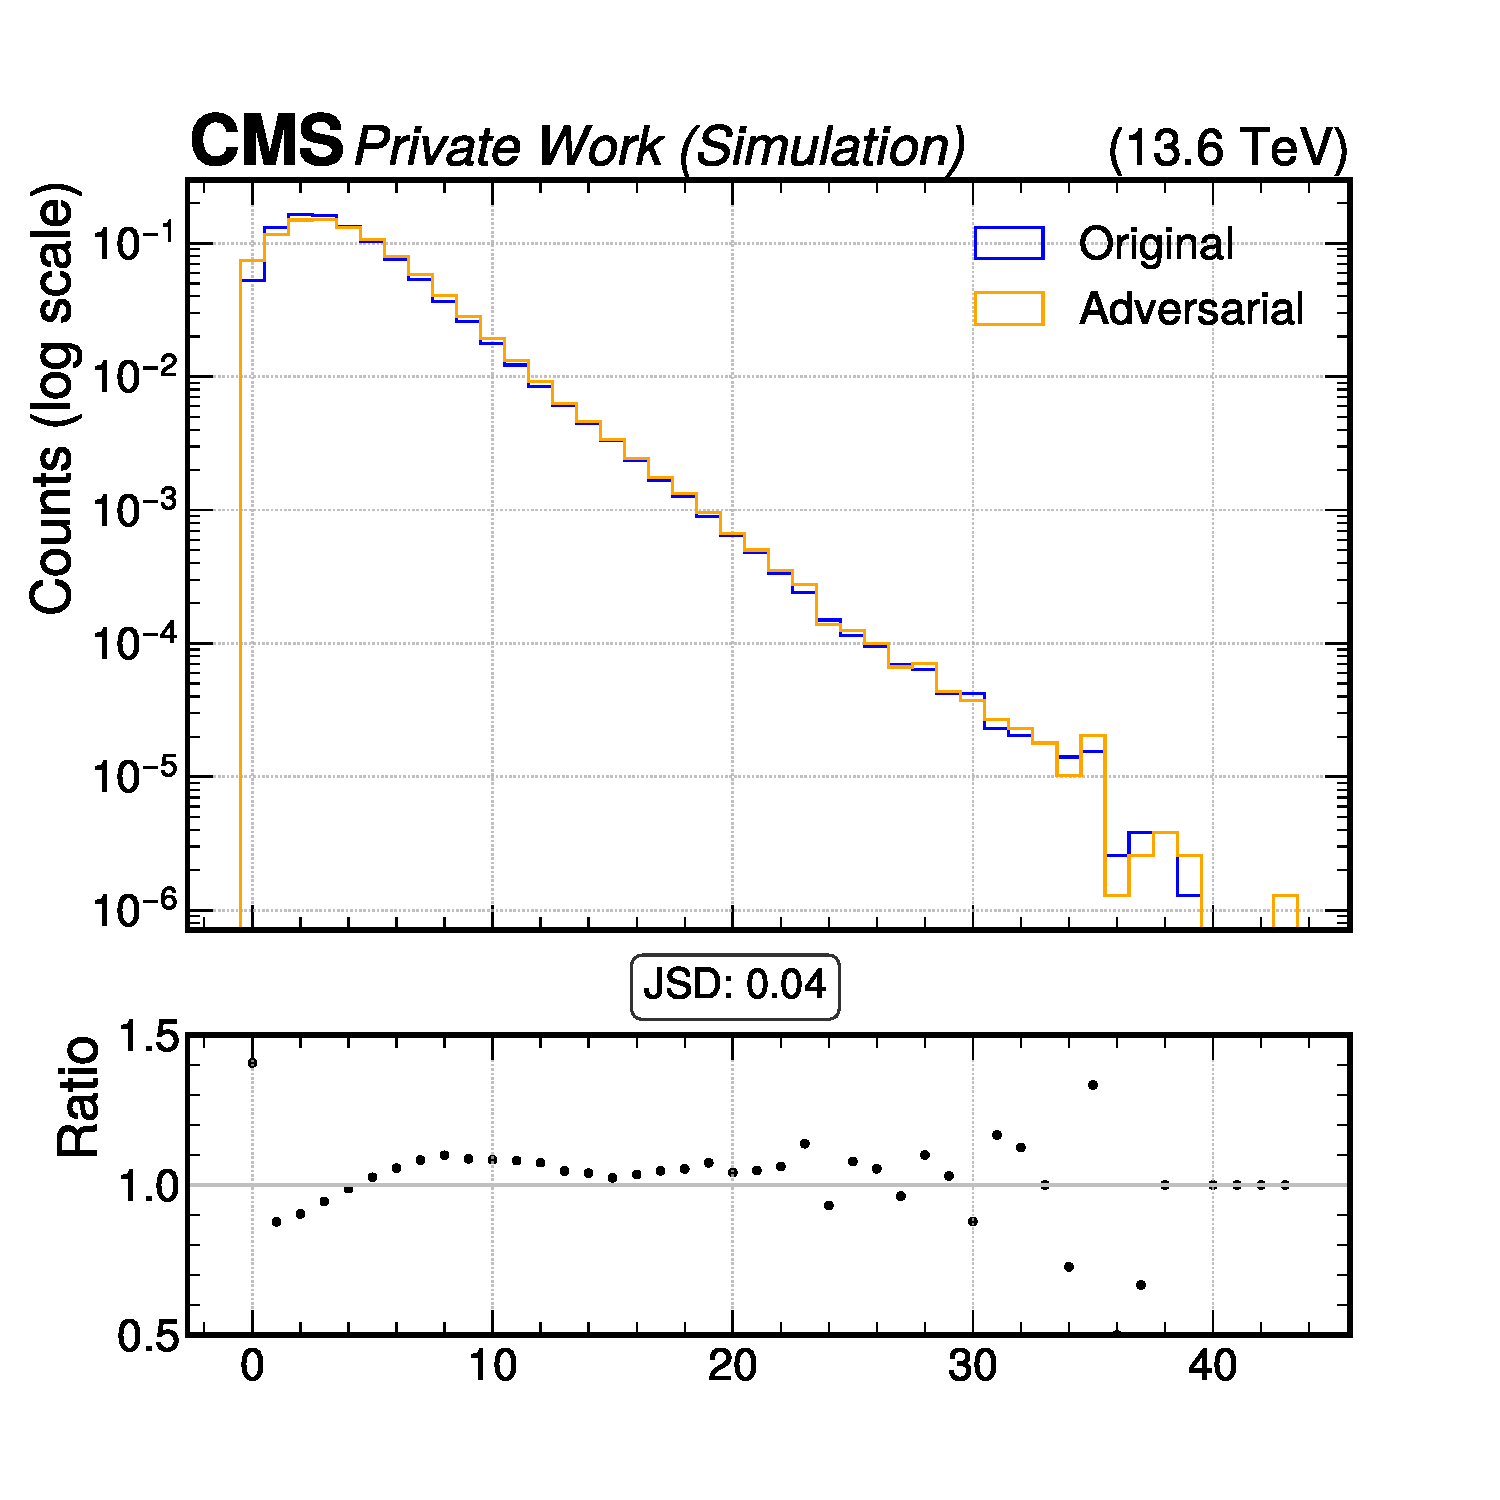
\includegraphics[width=\linewidth]{media/output/features/compare/intprob_3/cmp_global_features_n_Npfcand.pdf}
    \caption{Input similarity for PIP(3).}
  \end{subfigure}

  \caption{Histogram of \texttt{n\_Npfcand} for multiple iterations of PIP tested against nominal inputs.}
  \label{fig:intprob_input_n_Npfcand}
\end{figure}
\begin{figure}[h]
  \centering
  \begin{subfigure}[t]{0.32\textwidth}
    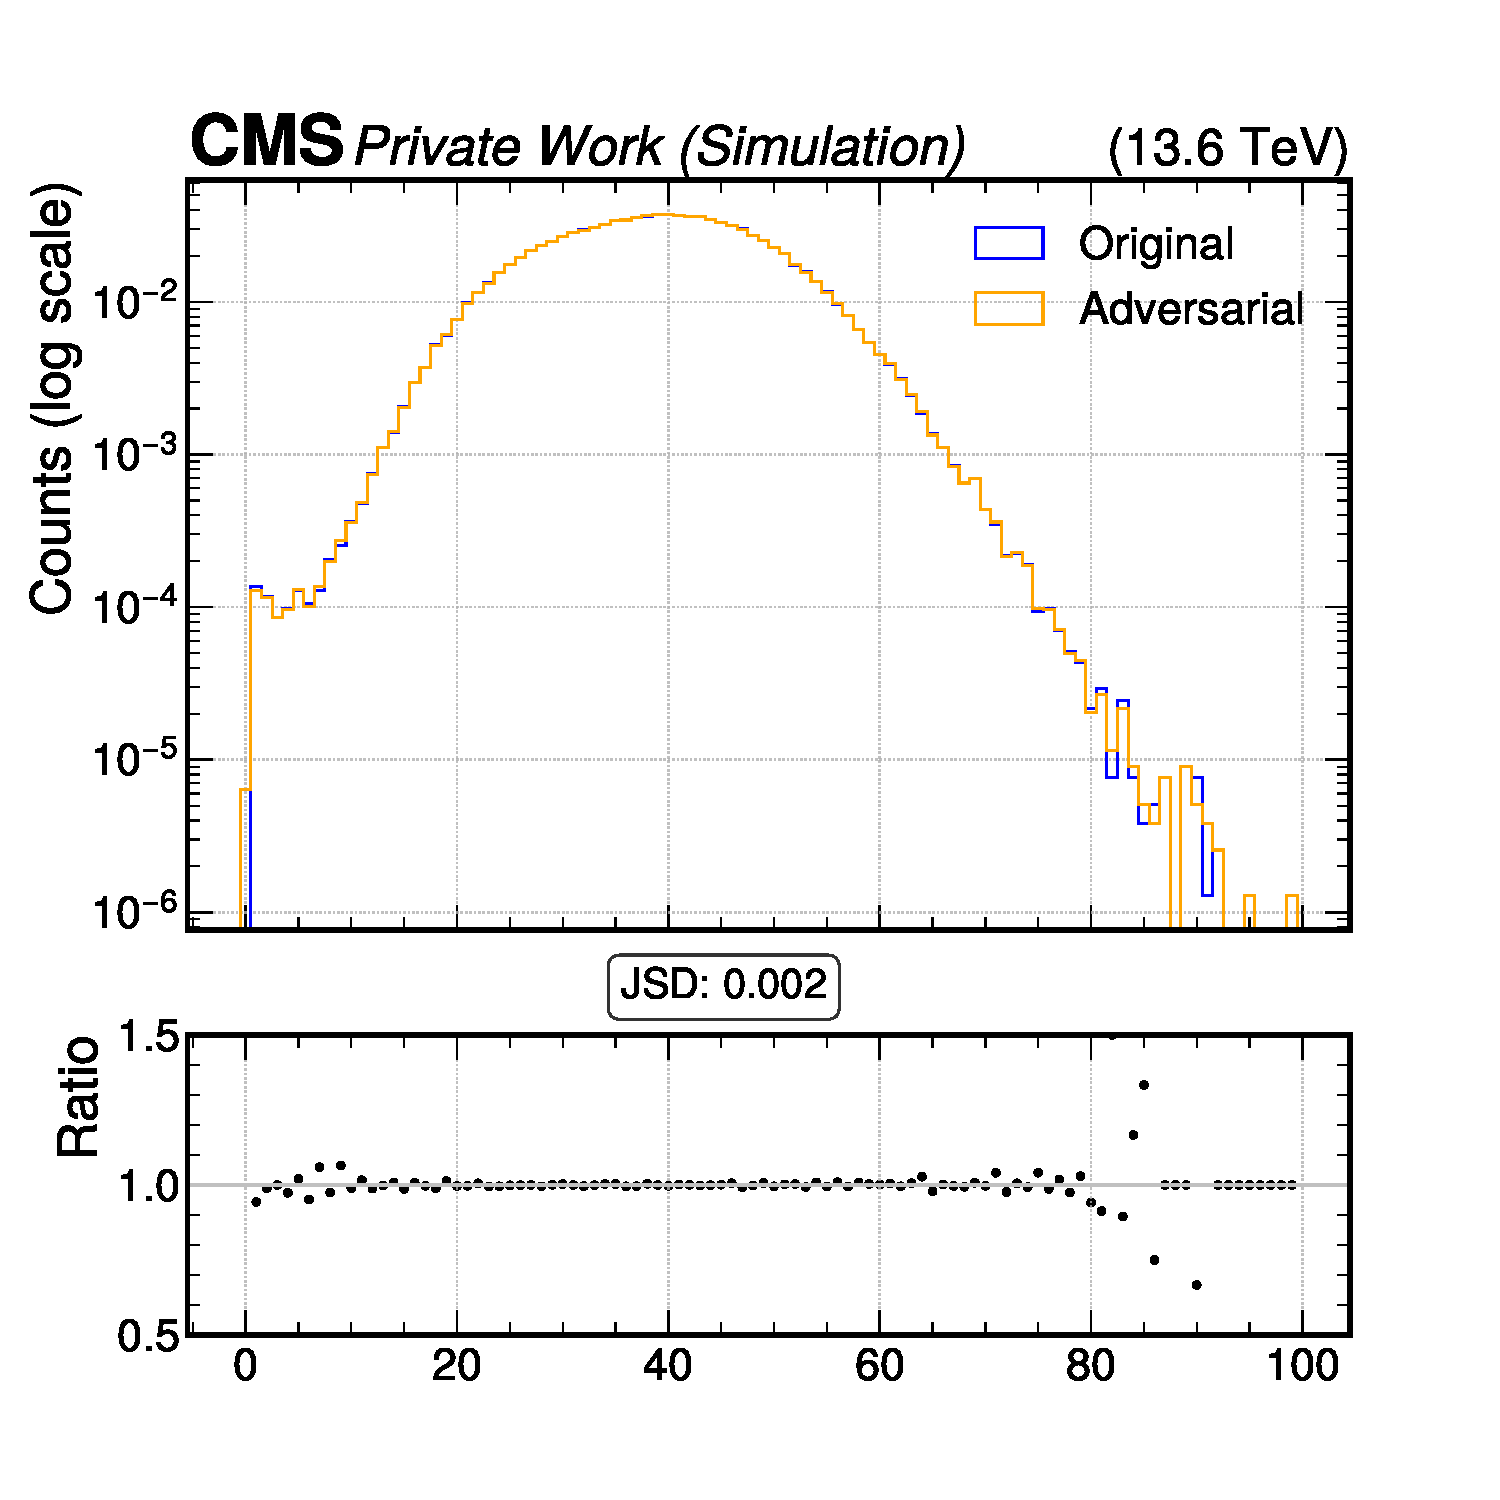
\includegraphics[width=\linewidth]{media/output/features/compare/intprob_1/cmp_global_features_npv.pdf}
    \caption{Input similarity for PIP(1).}
  \end{subfigure}\hfill
  \begin{subfigure}[t]{0.32\textwidth}
    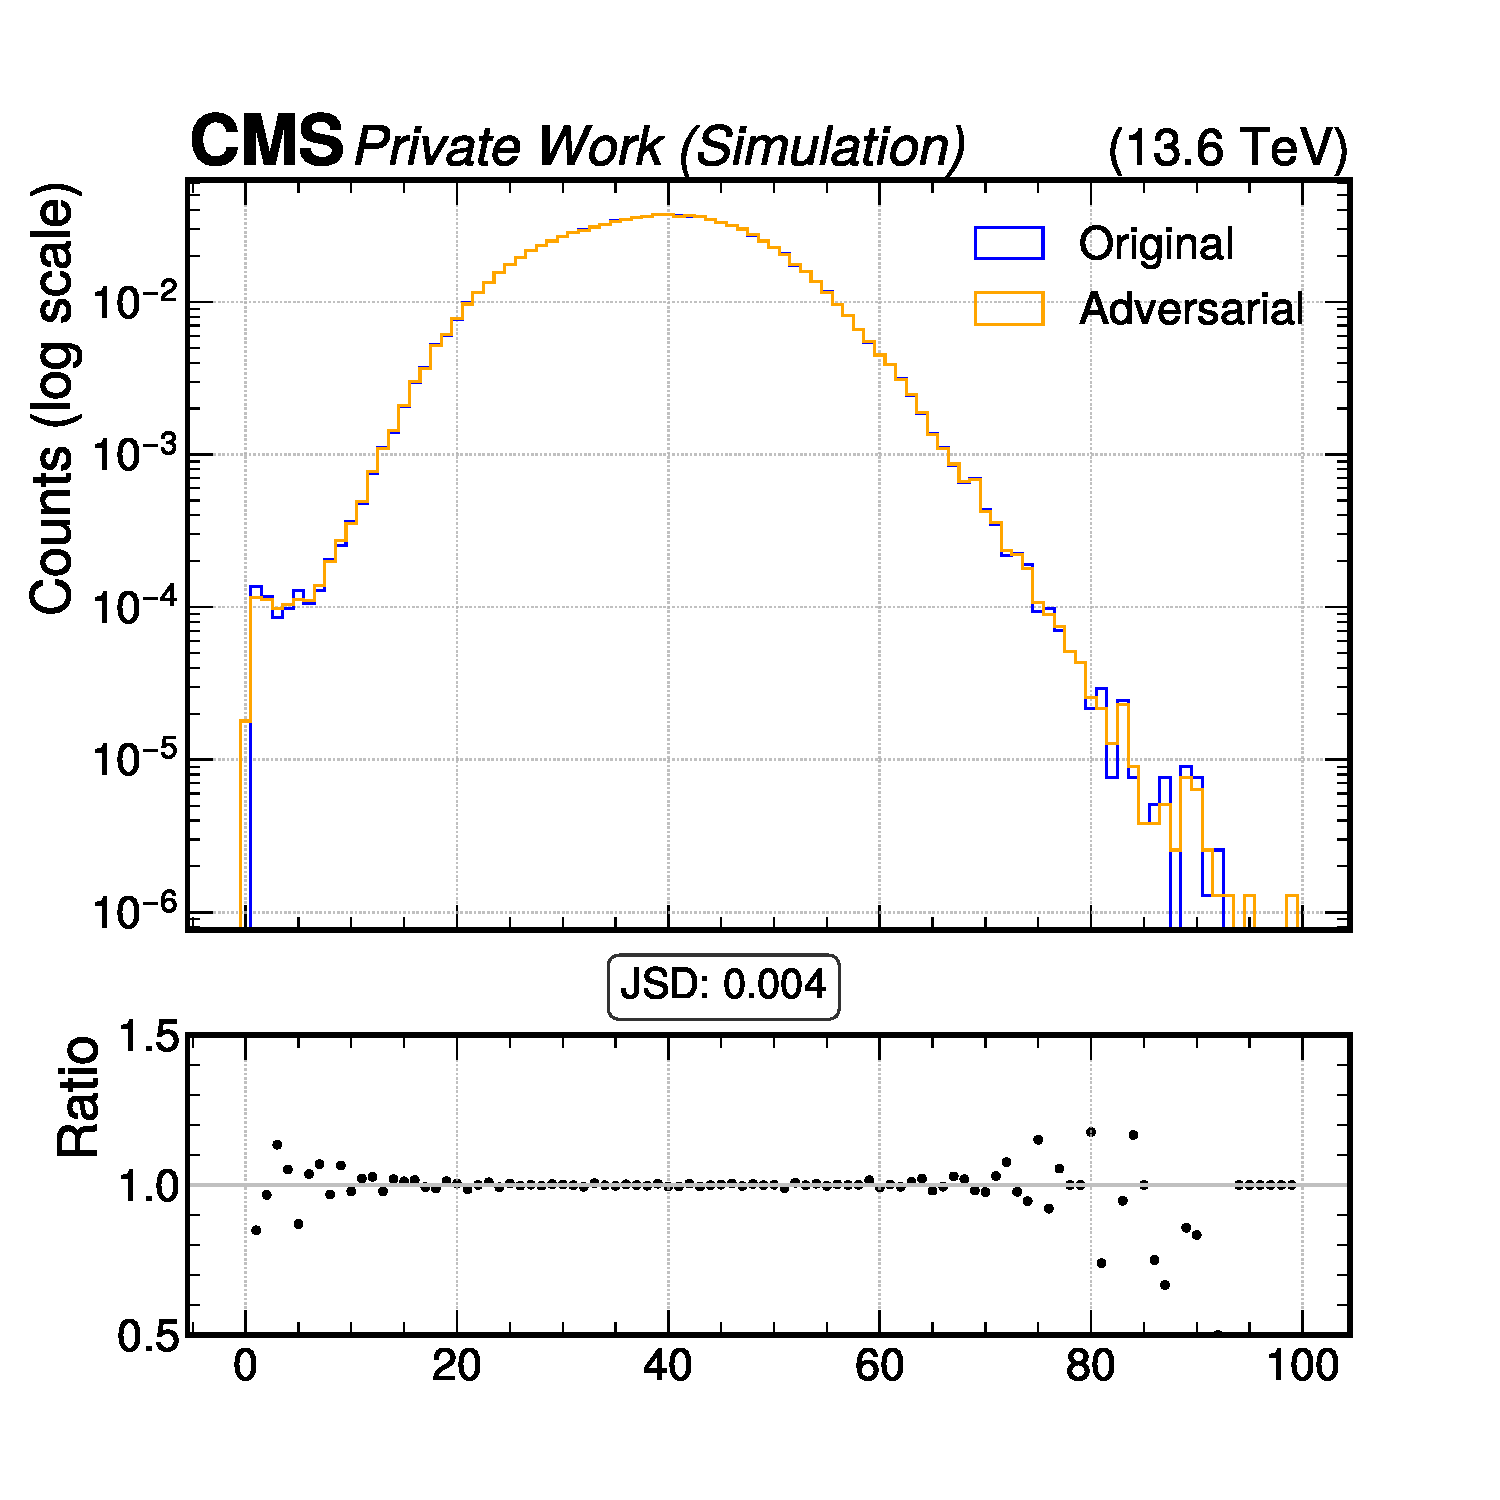
\includegraphics[width=\linewidth]{media/output/features/compare/intprob_2/cmp_global_features_npv.pdf}
    \caption{Input similarity for PIP(2).}
  \end{subfigure}\hfill
  \begin{subfigure}[t]{0.32\textwidth}
    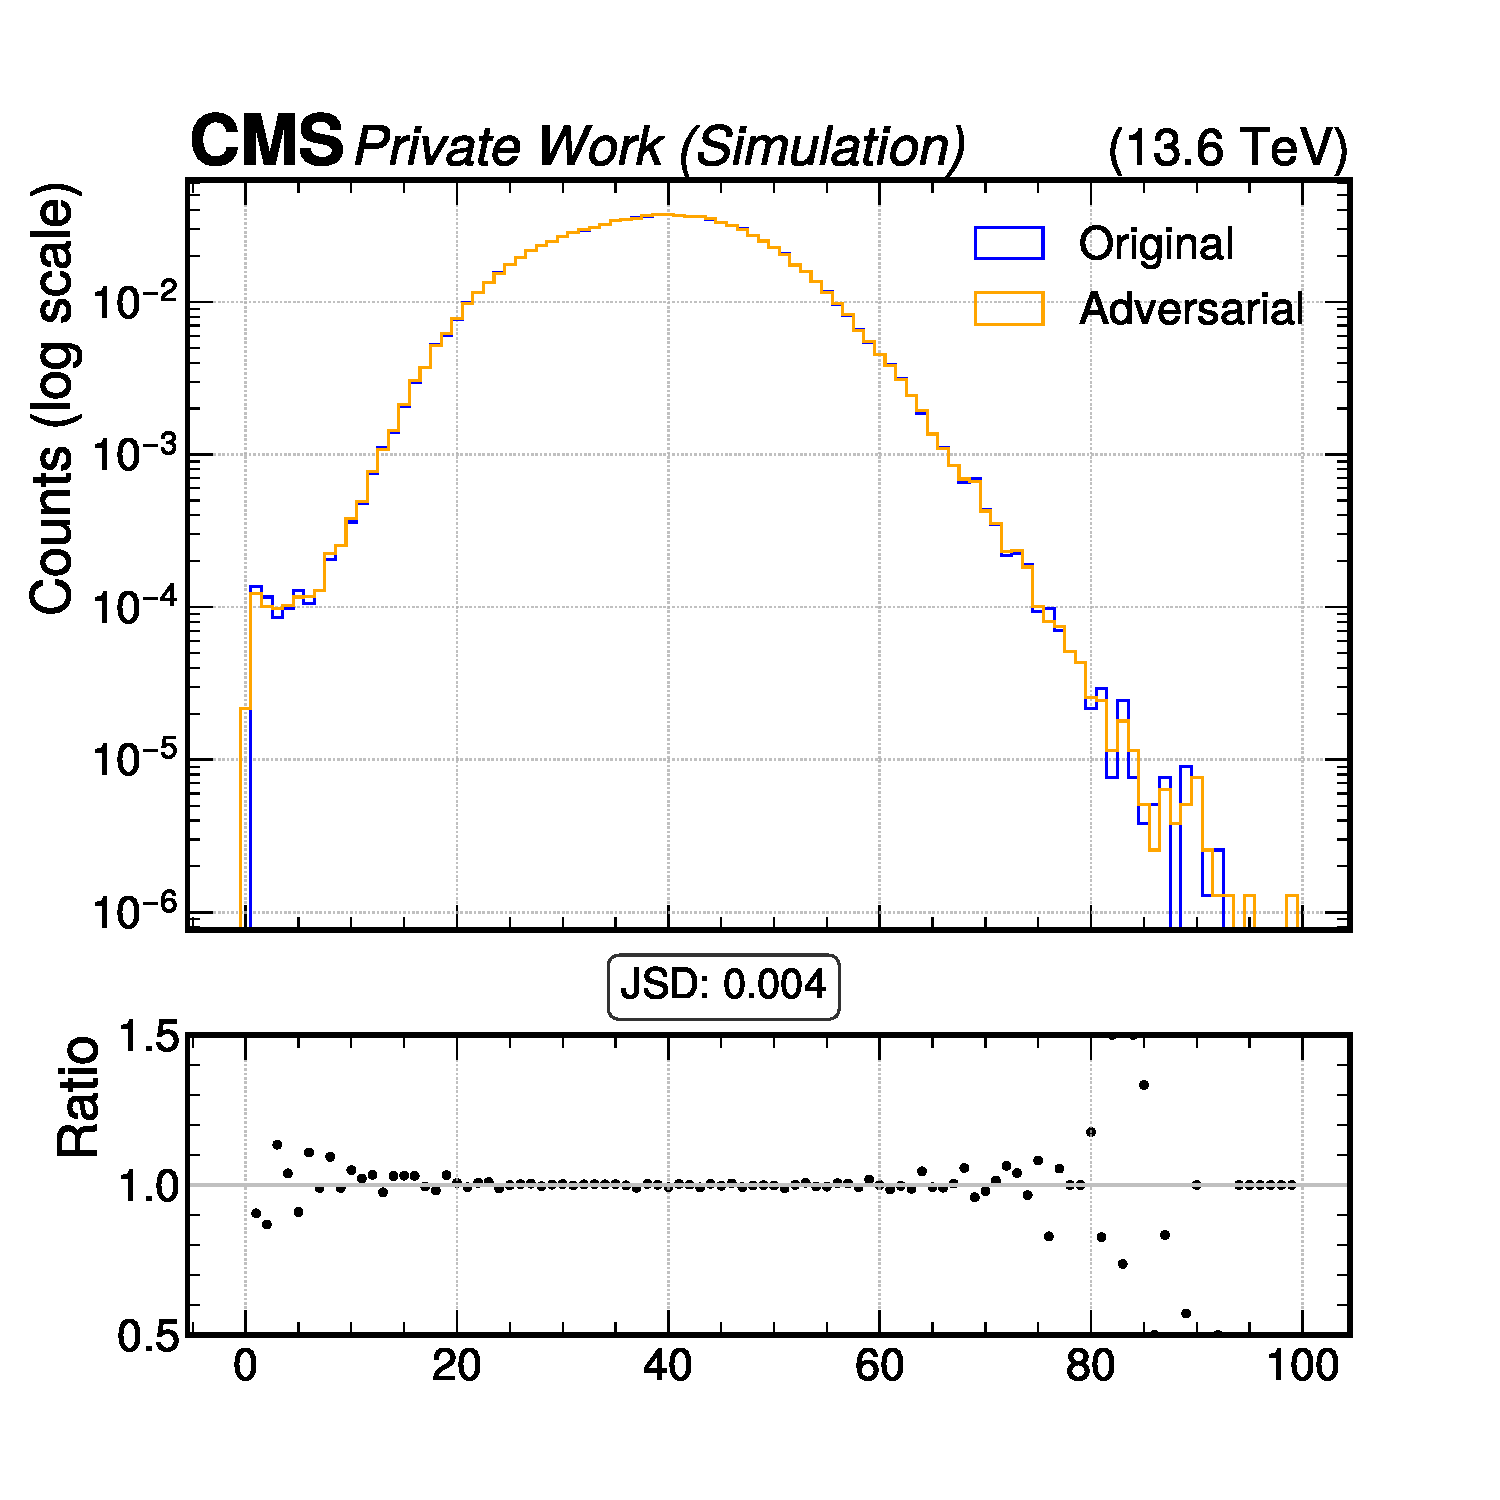
\includegraphics[width=\linewidth]{media/output/features/compare/intprob_3/cmp_global_features_npv.pdf}
    \caption{Input similarity for PIP(3).}
  \end{subfigure}

  \caption{Histogram of \texttt{npv} for multiple iterations of PIP tested against nominal inputs.}
  \label{fig:intprob_input_npv}
\end{figure}
\begin{figure}[h]
  \centering
  \begin{subfigure}[t]{0.32\textwidth}
    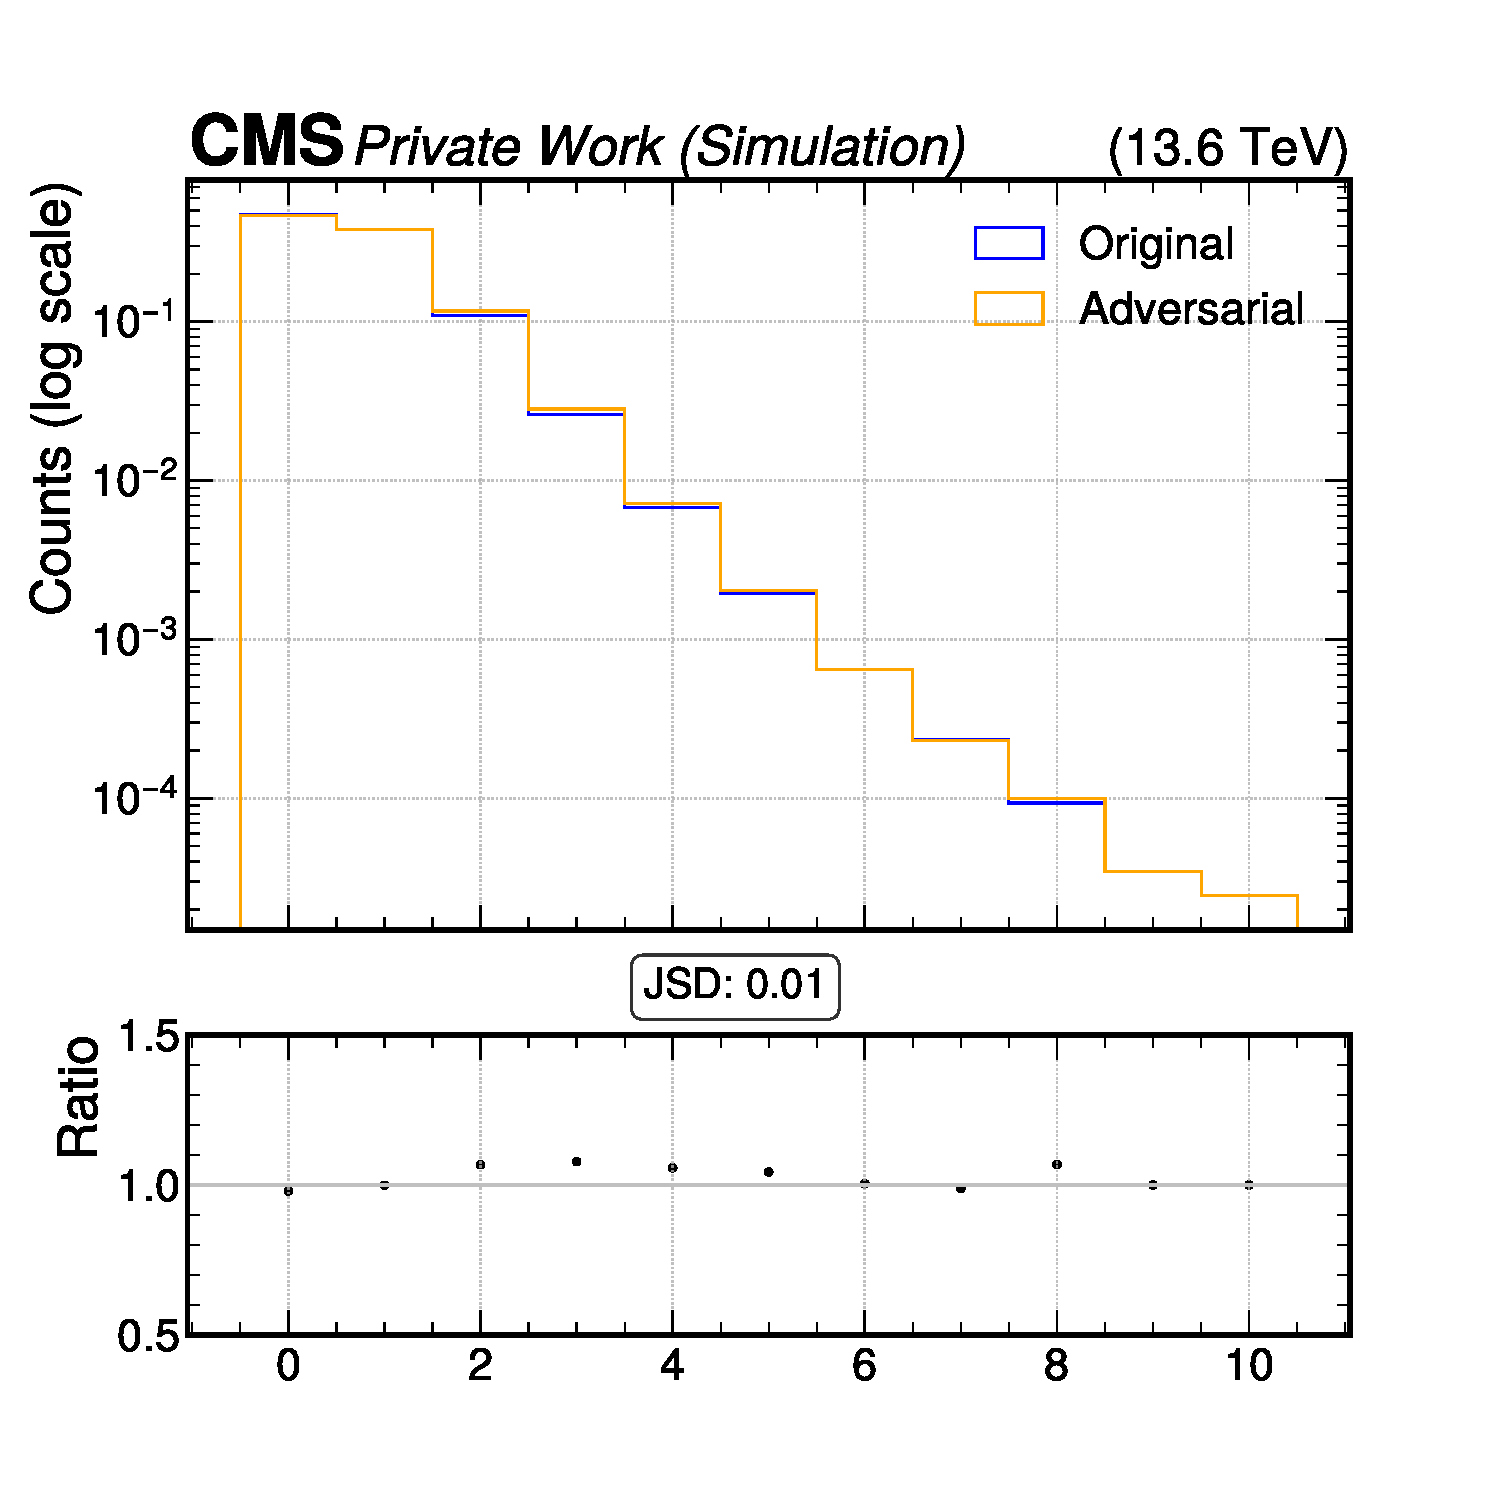
\includegraphics[width=\linewidth]{media/output/features/compare/intprob_1/cmp_global_features_nsv.pdf}
    \caption{Input similarity for PIP(1).}
  \end{subfigure}\hfill
  \begin{subfigure}[t]{0.32\textwidth}
    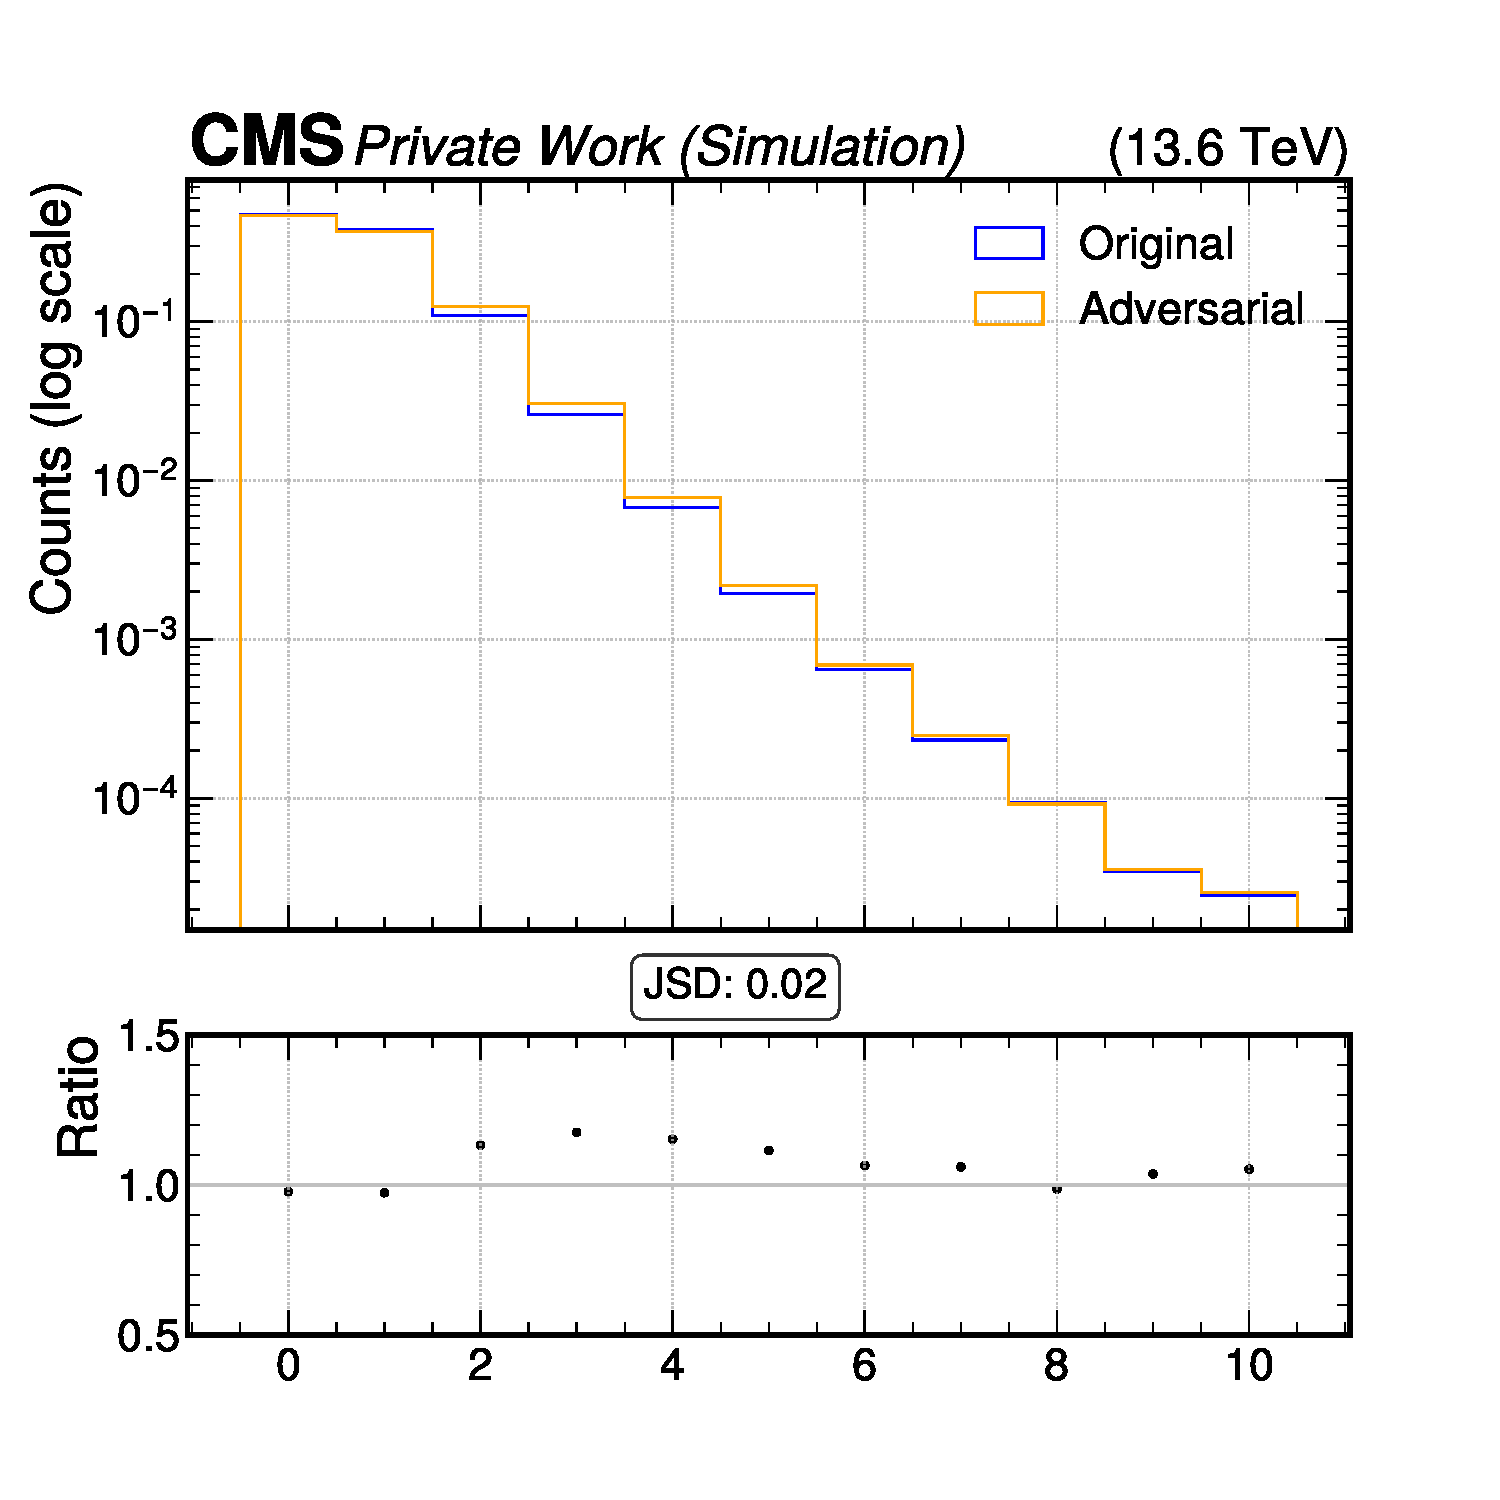
\includegraphics[width=\linewidth]{media/output/features/compare/intprob_2/cmp_global_features_nsv.pdf}
    \caption{Input similarity for PIP(2).}
  \end{subfigure}\hfill
  \begin{subfigure}[t]{0.32\textwidth}
    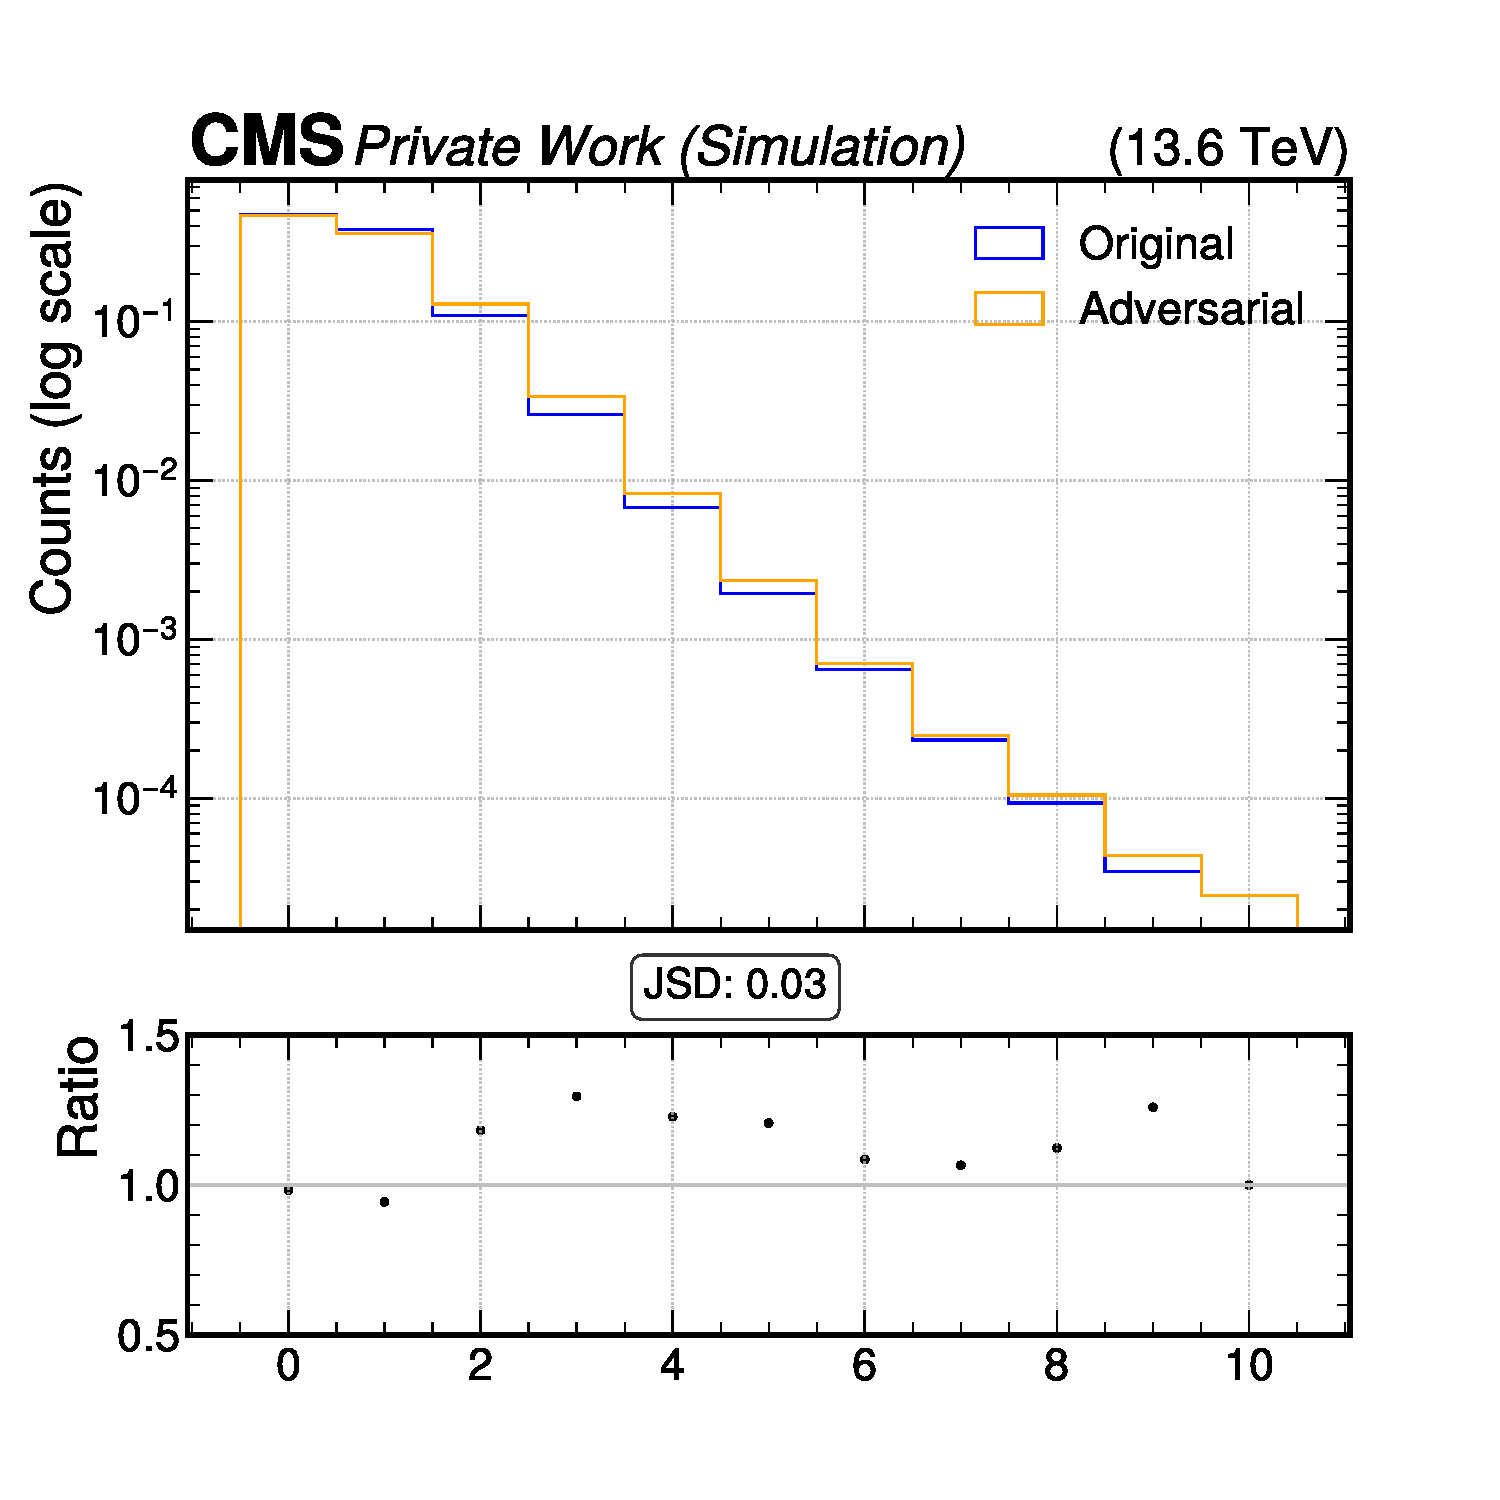
\includegraphics[width=\linewidth]{media/output/features/compare/intprob_3/cmp_global_features_nsv.pdf}
    \caption{Input similarity for PIP(3).}
  \end{subfigure}

  \caption{Histogram of \texttt{nsv} for multiple iterations of PIP tested against nominal inputs.}
  \label{fig:intprob_input_nsv}
\end{figure}
\begin{figure}[h]
  \centering
  \begin{subfigure}[t]{0.32\textwidth}
    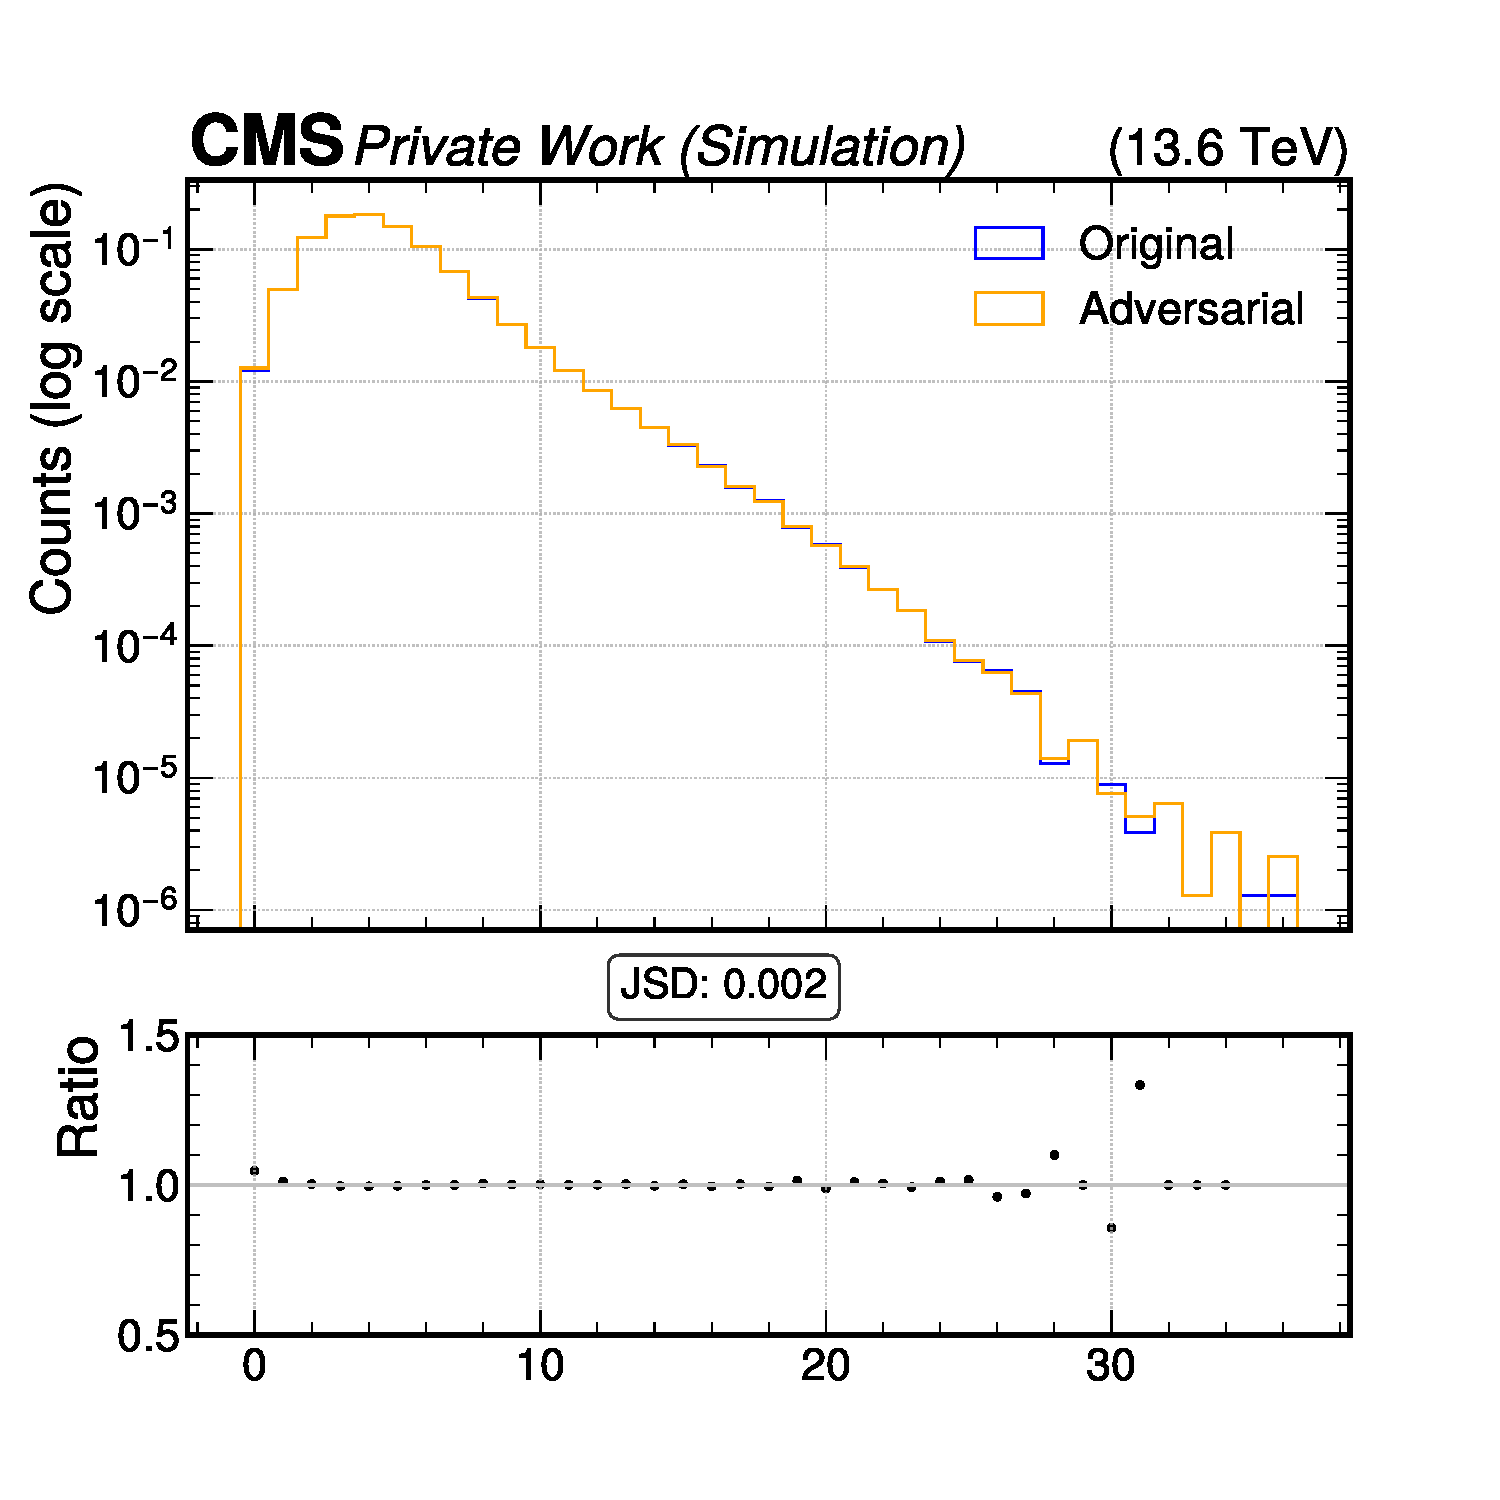
\includegraphics[width=\linewidth]{media/output/features/compare/intprob_1/cmp_global_features_TagVarCSV_jetNSelectedTracks.pdf}
    \caption{Input similarity for PIP(1).}
  \end{subfigure}\hfill
  \begin{subfigure}[t]{0.32\textwidth}
    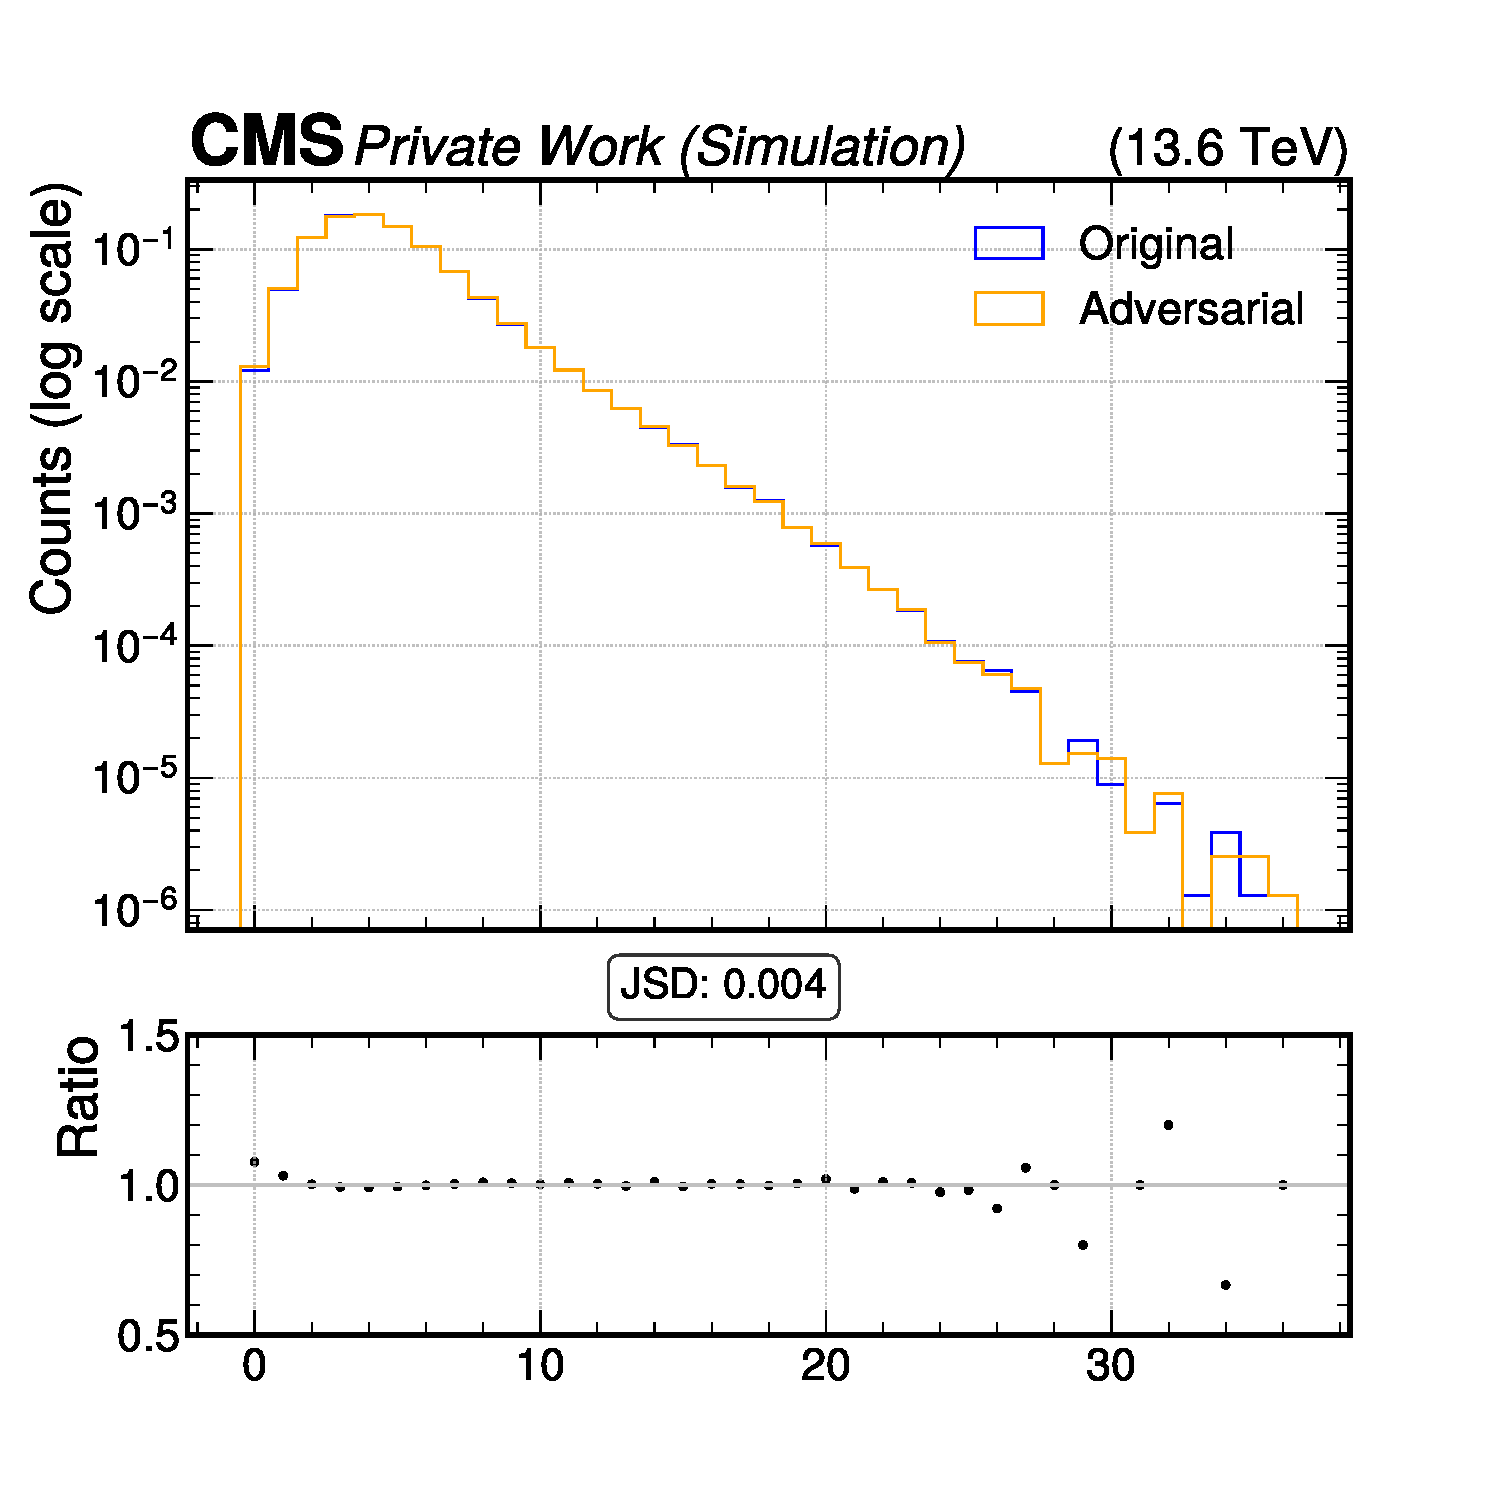
\includegraphics[width=\linewidth]{media/output/features/compare/intprob_2/cmp_global_features_TagVarCSV_jetNSelectedTracks.pdf}
    \caption{Input similarity for PIP(2).}
  \end{subfigure}\hfill
  \begin{subfigure}[t]{0.32\textwidth}
    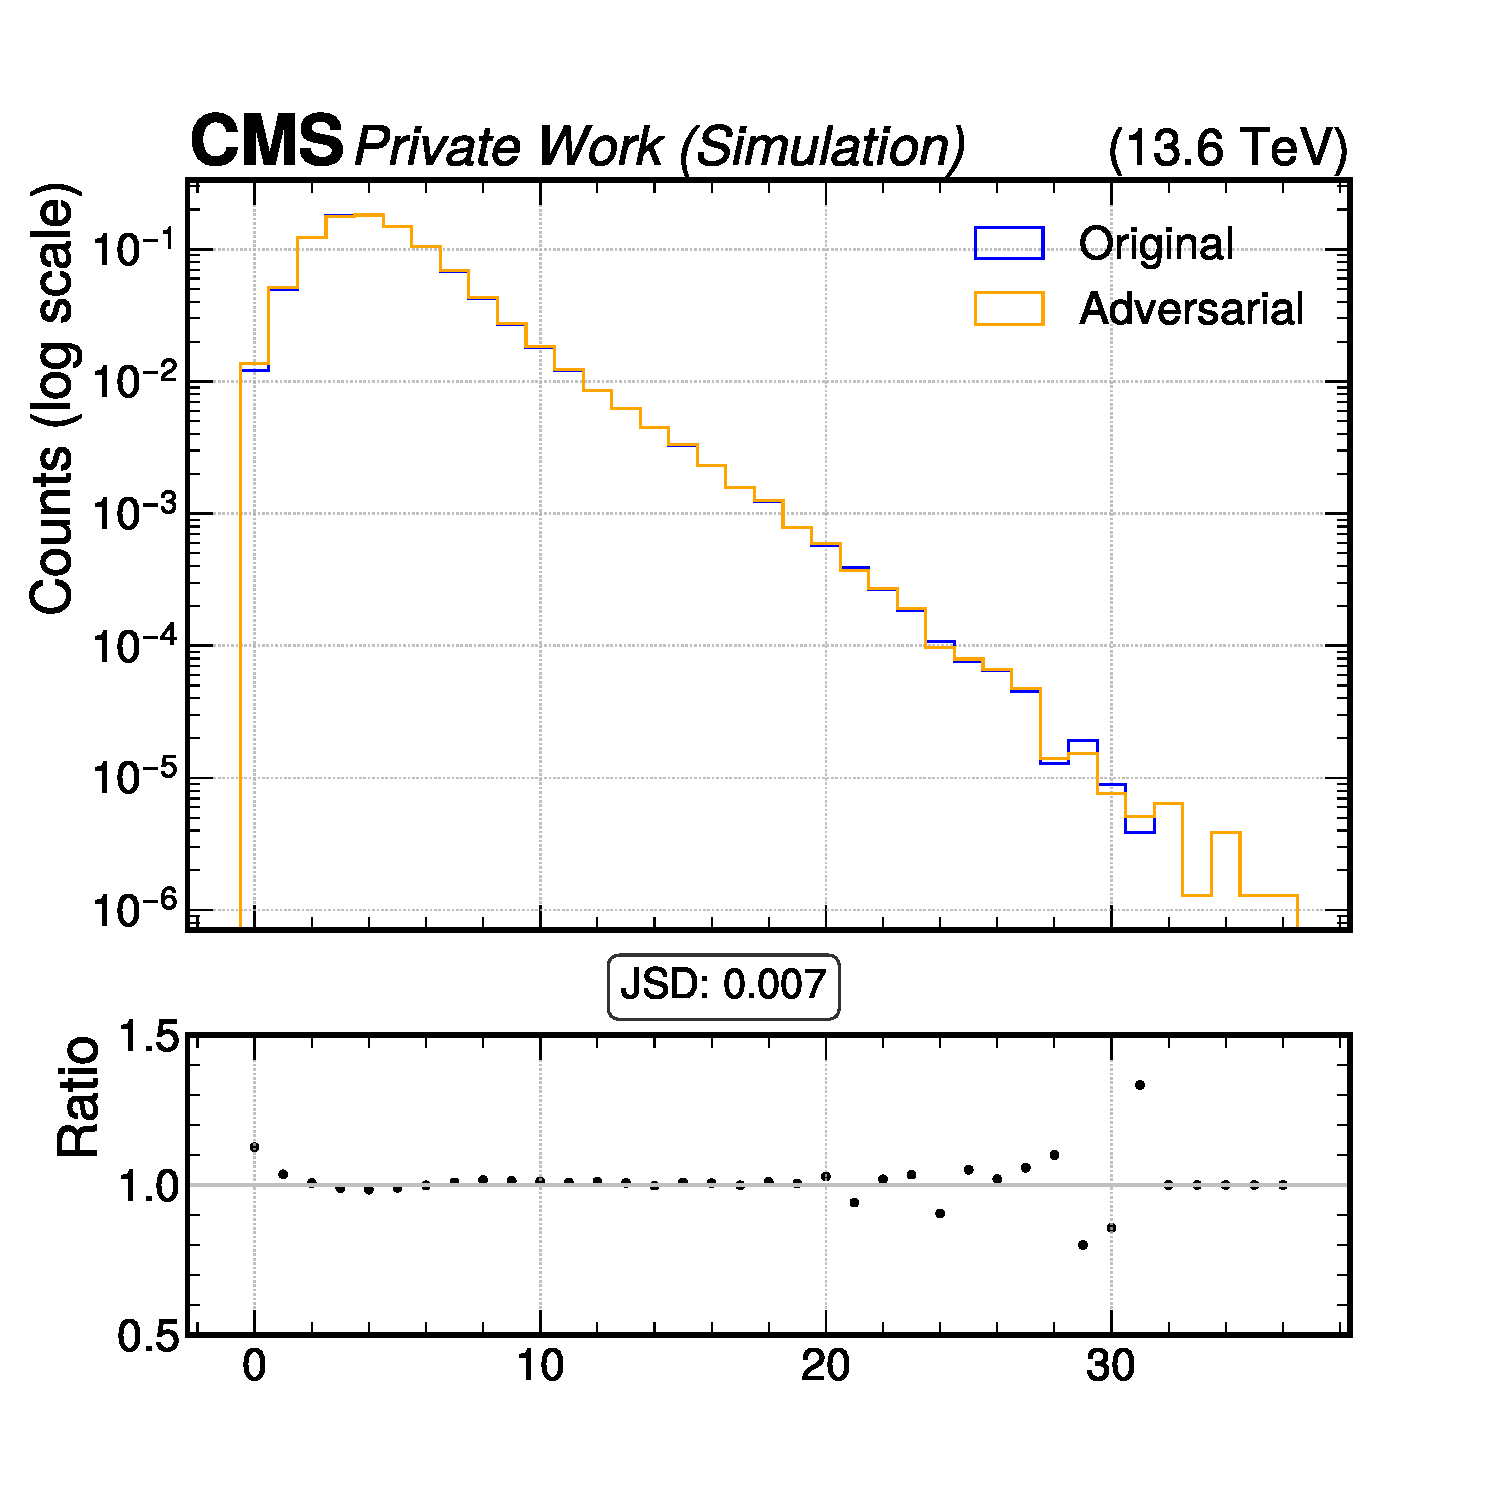
\includegraphics[width=\linewidth]{media/output/features/compare/intprob_3/cmp_global_features_TagVarCSV_jetNSelectedTracks.pdf}
    \caption{Input similarity for PIP(3).}
  \end{subfigure}

  \caption{Histogram of \texttt{TagVarCSV\_jetNSelectedTracks} for multiple iterations of PIP tested against nominal inputs.}
  \label{fig:intprob_input_TagVarCSV_jetNSelectedTracks}
\end{figure}
\begin{figure}[h]
  \centering
  \begin{subfigure}[t]{0.32\textwidth}
    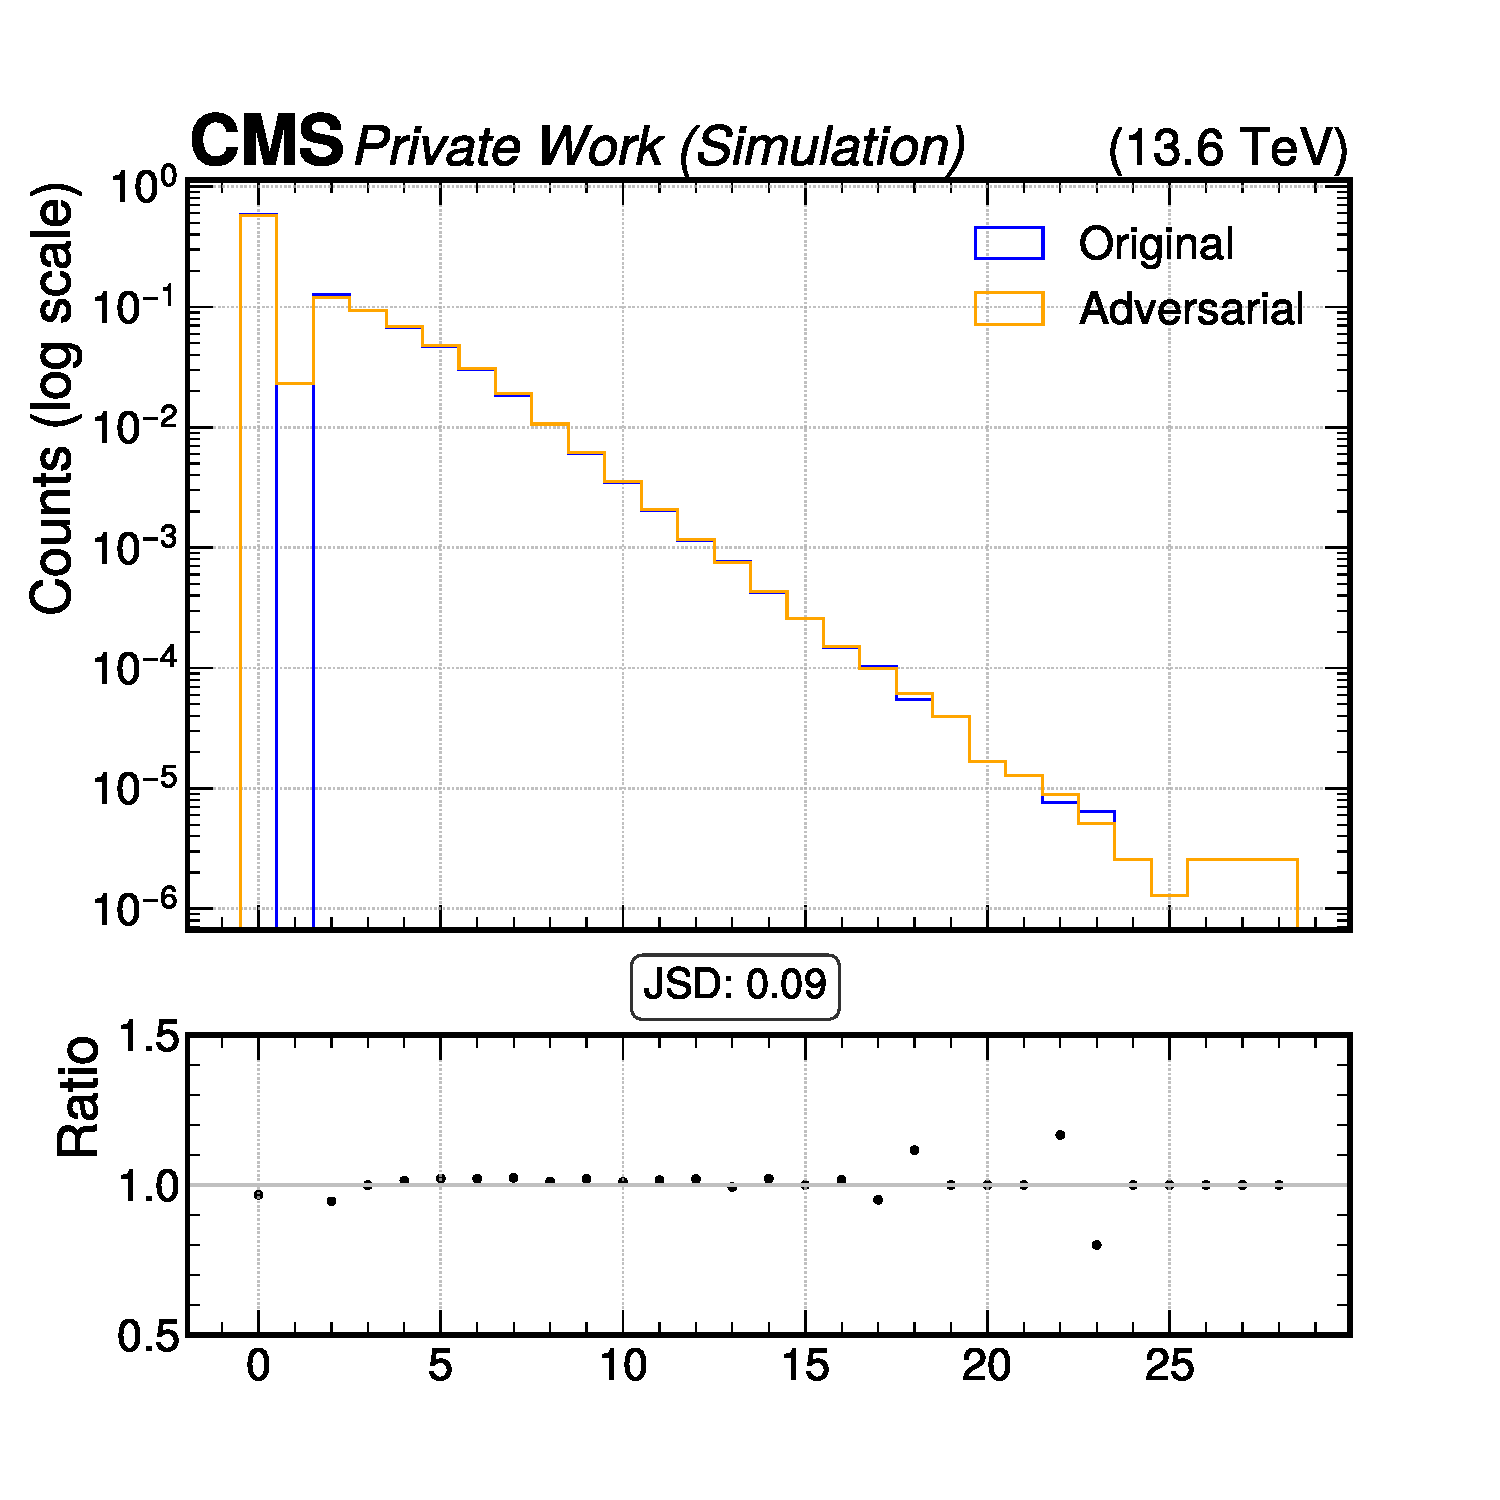
\includegraphics[width=\linewidth]{media/output/features/compare/intprob_1/cmp_global_features_TagVarCSV_jetNTracksEtaRel.pdf}
    \caption{Input similarity for PIP(1).}
  \end{subfigure}\hfill
  \begin{subfigure}[t]{0.32\textwidth}
    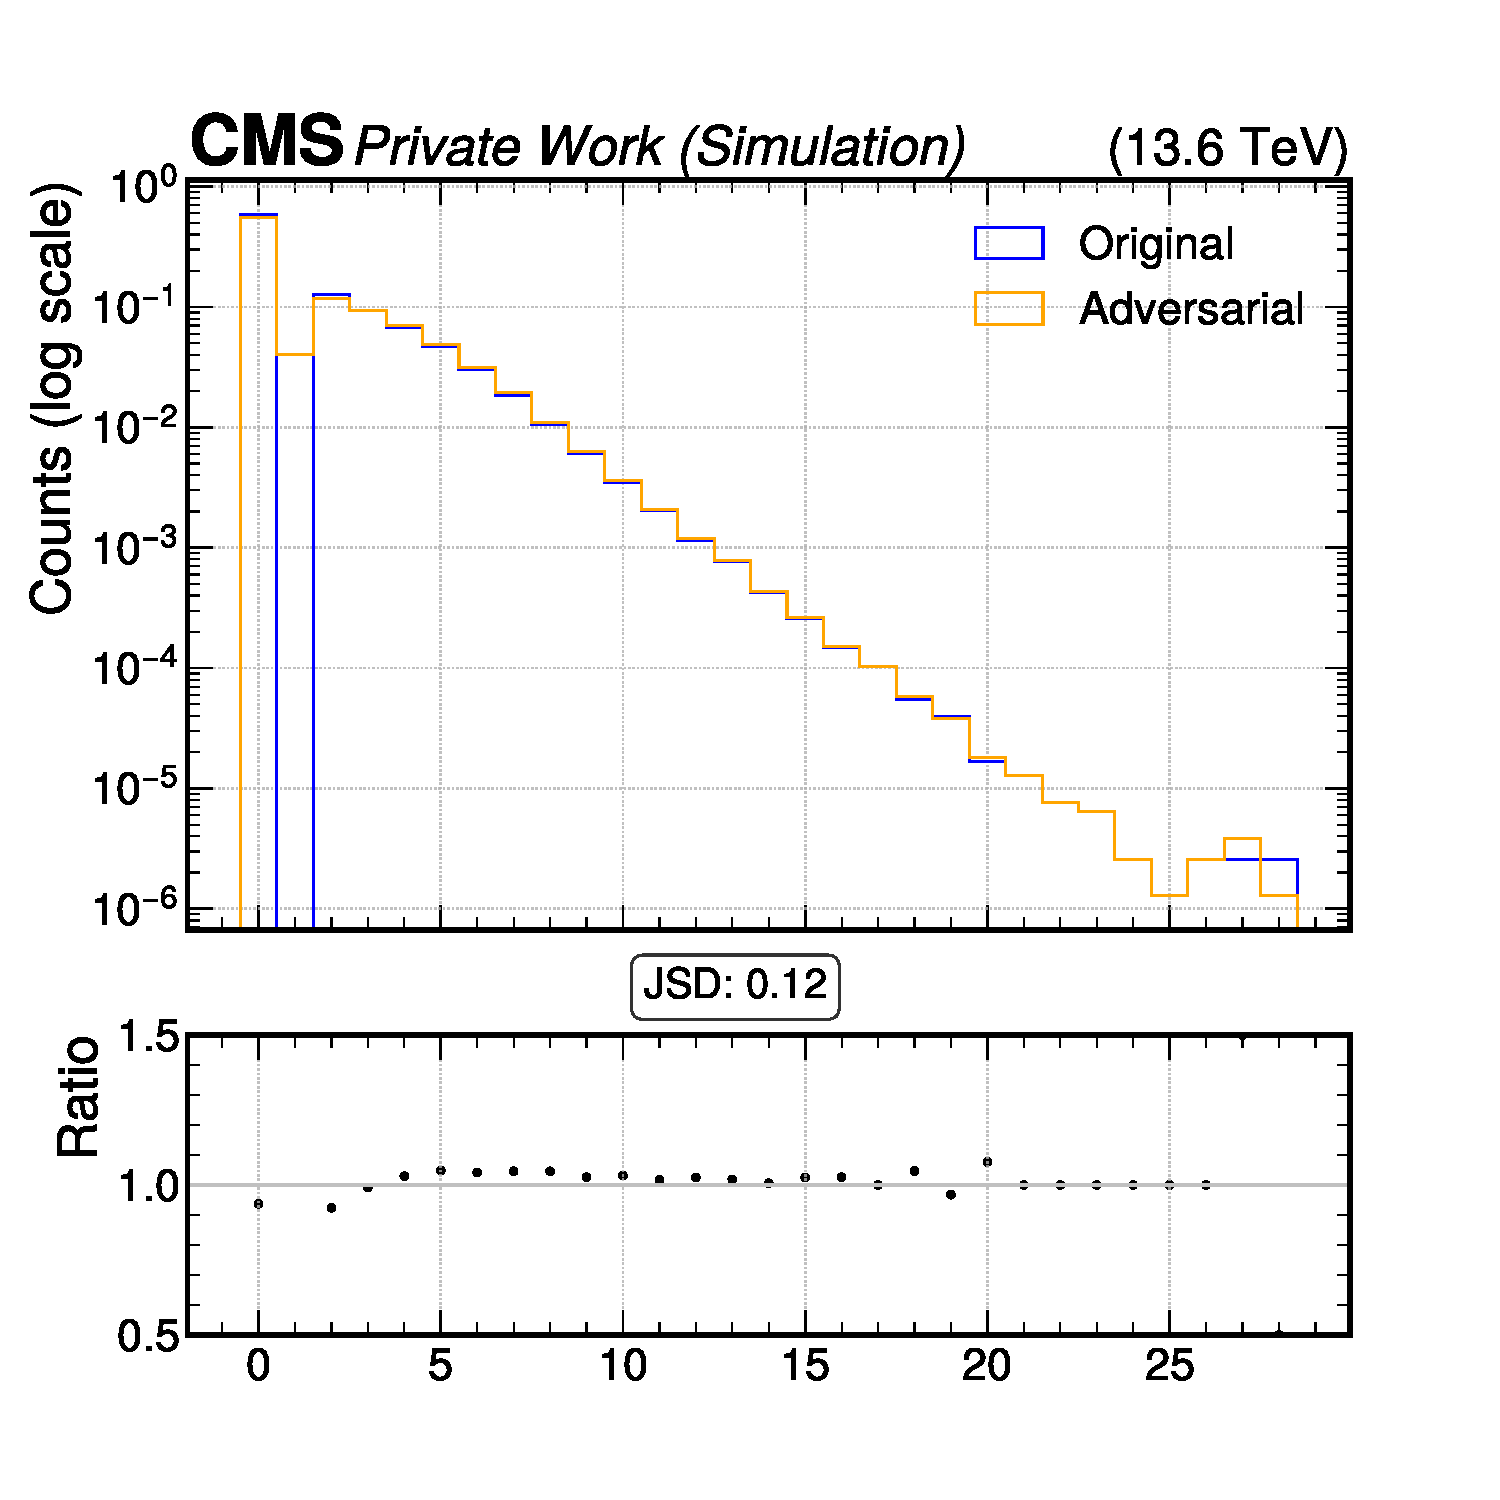
\includegraphics[width=\linewidth]{media/output/features/compare/intprob_2/cmp_global_features_TagVarCSV_jetNTracksEtaRel.pdf}
    \caption{Input similarity for PIP(2).}
  \end{subfigure}\hfill
  \begin{subfigure}[t]{0.32\textwidth}
    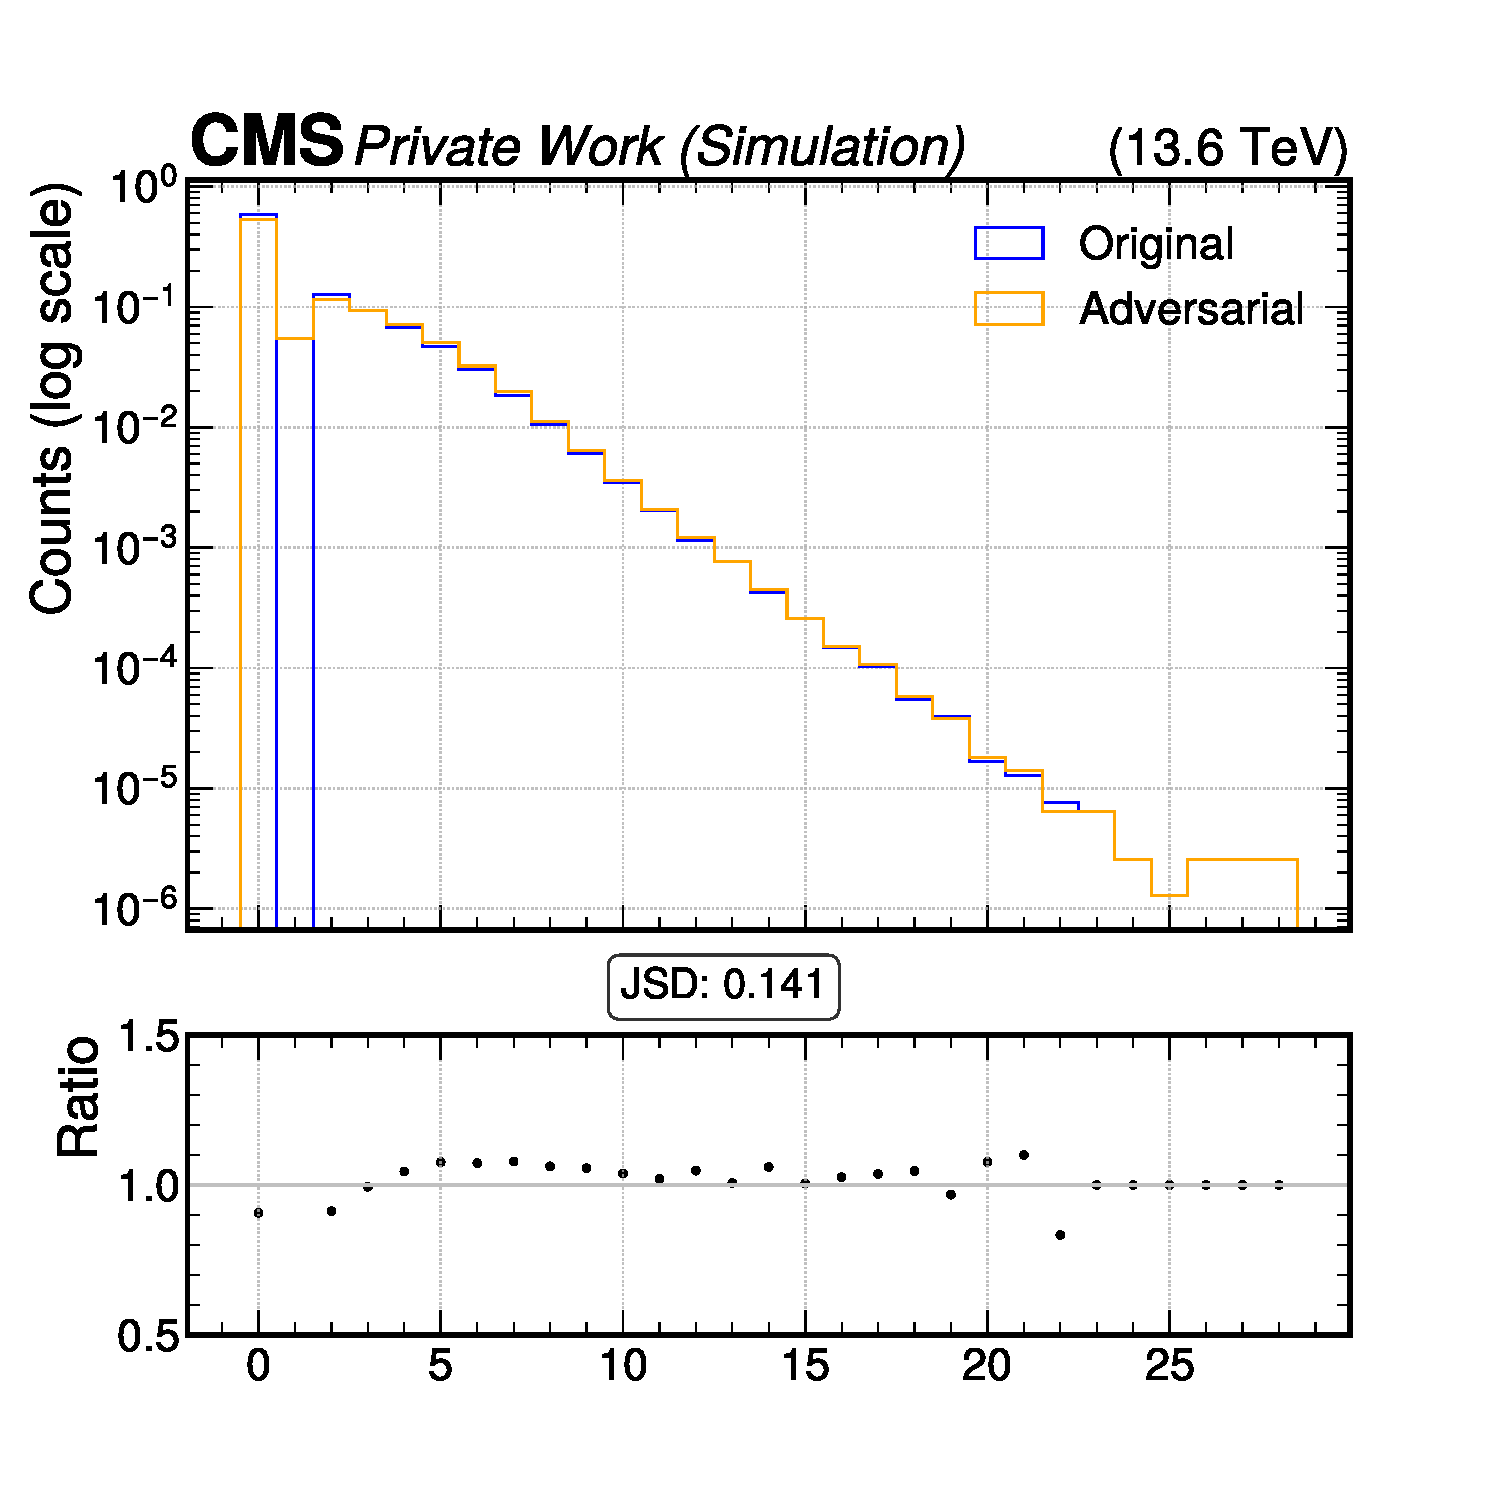
\includegraphics[width=\linewidth]{media/output/features/compare/intprob_3/cmp_global_features_TagVarCSV_jetNTracksEtaRel.pdf}
    \caption{Input similarity for PIP(3).}
  \end{subfigure}

  \caption{Histogram of \texttt{TagVarCSV\_jetNTracksEtaRel} for multiple iterations of PIP tested against nominal inputs.}
  \label{fig:intprob_input_TagVarCSV_jetNTracksEtaRel}
\end{figure}
\begin{figure}[h]
  \centering
  \begin{subfigure}[t]{0.32\textwidth}
    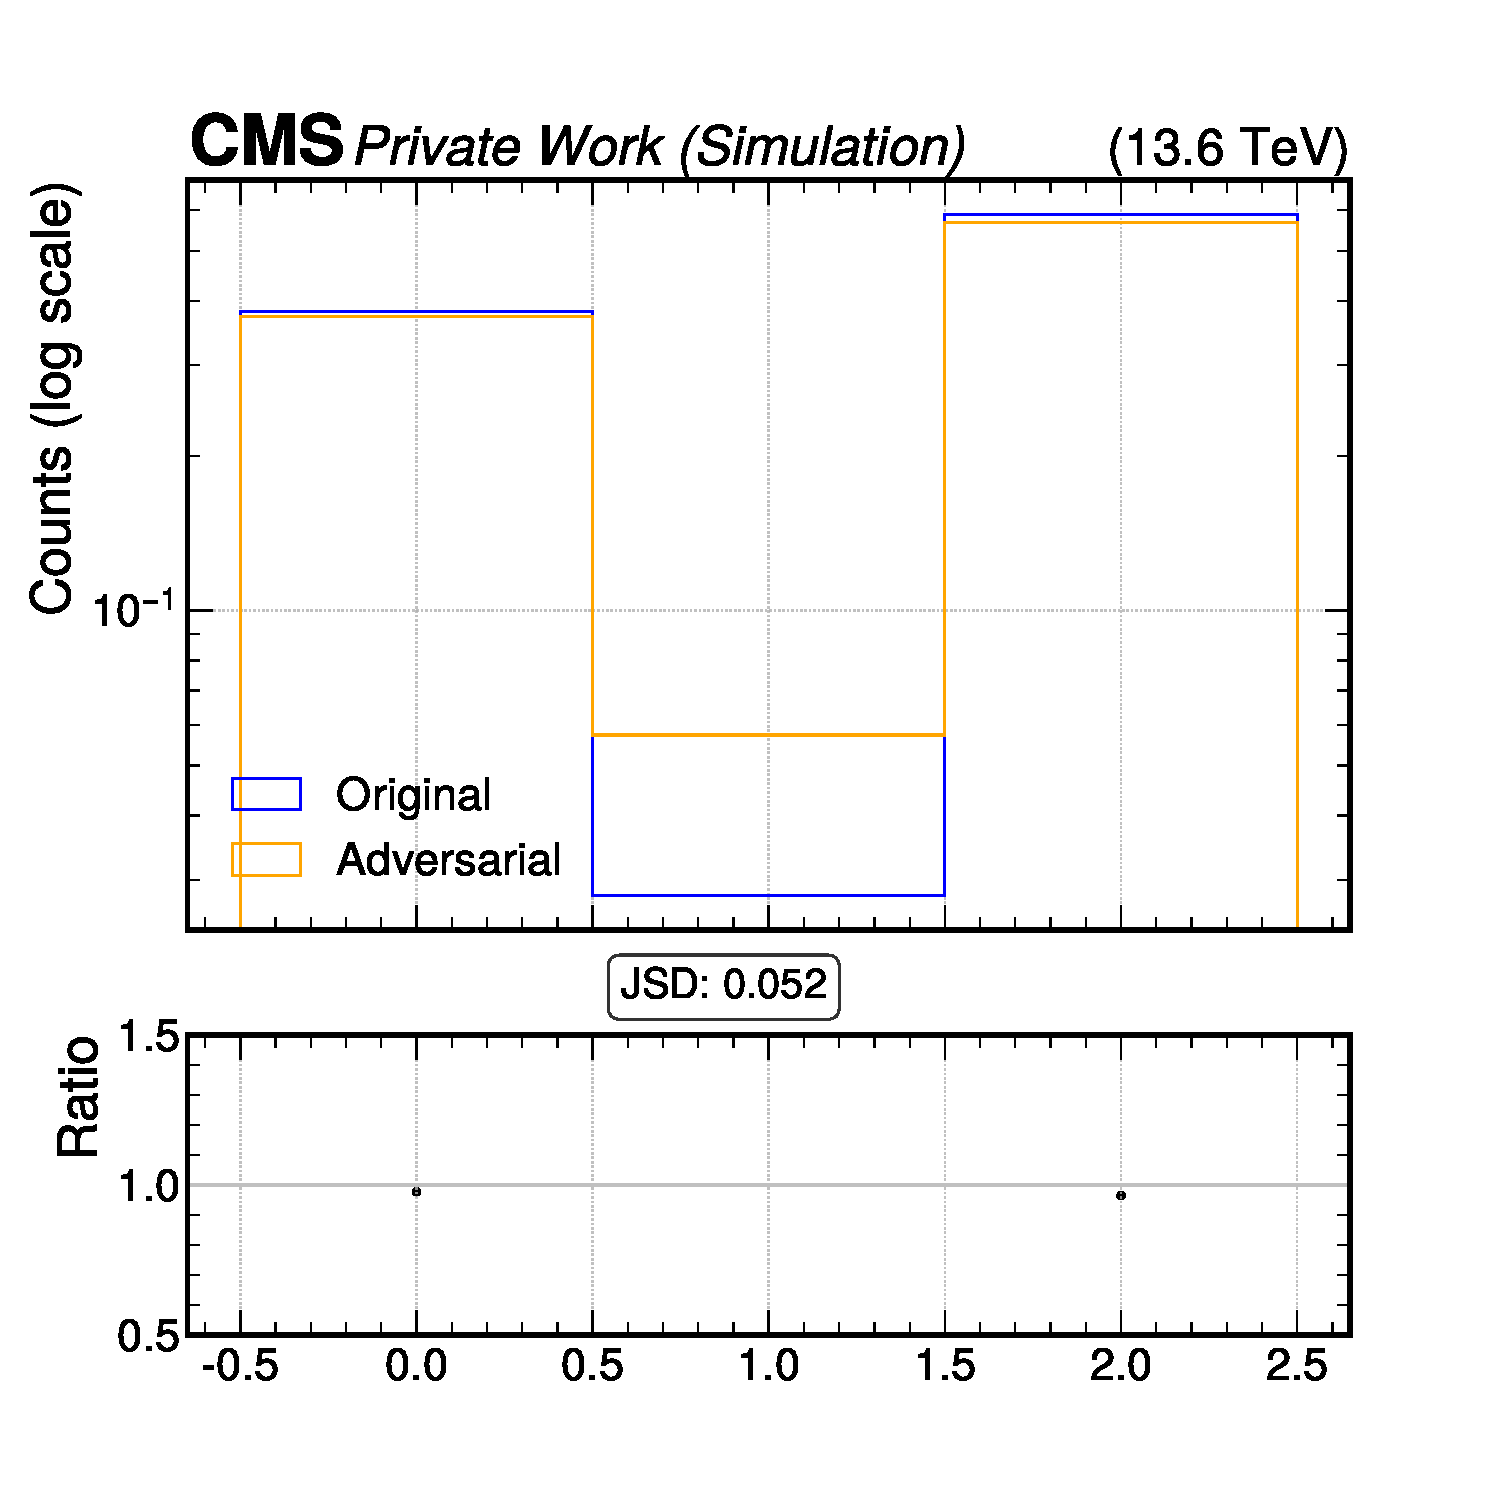
\includegraphics[width=\linewidth]{media/output/features/compare/intprob_1/cmp_global_features_TagVarCSV_vertexCategory.pdf}
    \caption{Input similarity for PIP(1).}
  \end{subfigure}\hfill
  \begin{subfigure}[t]{0.32\textwidth}
    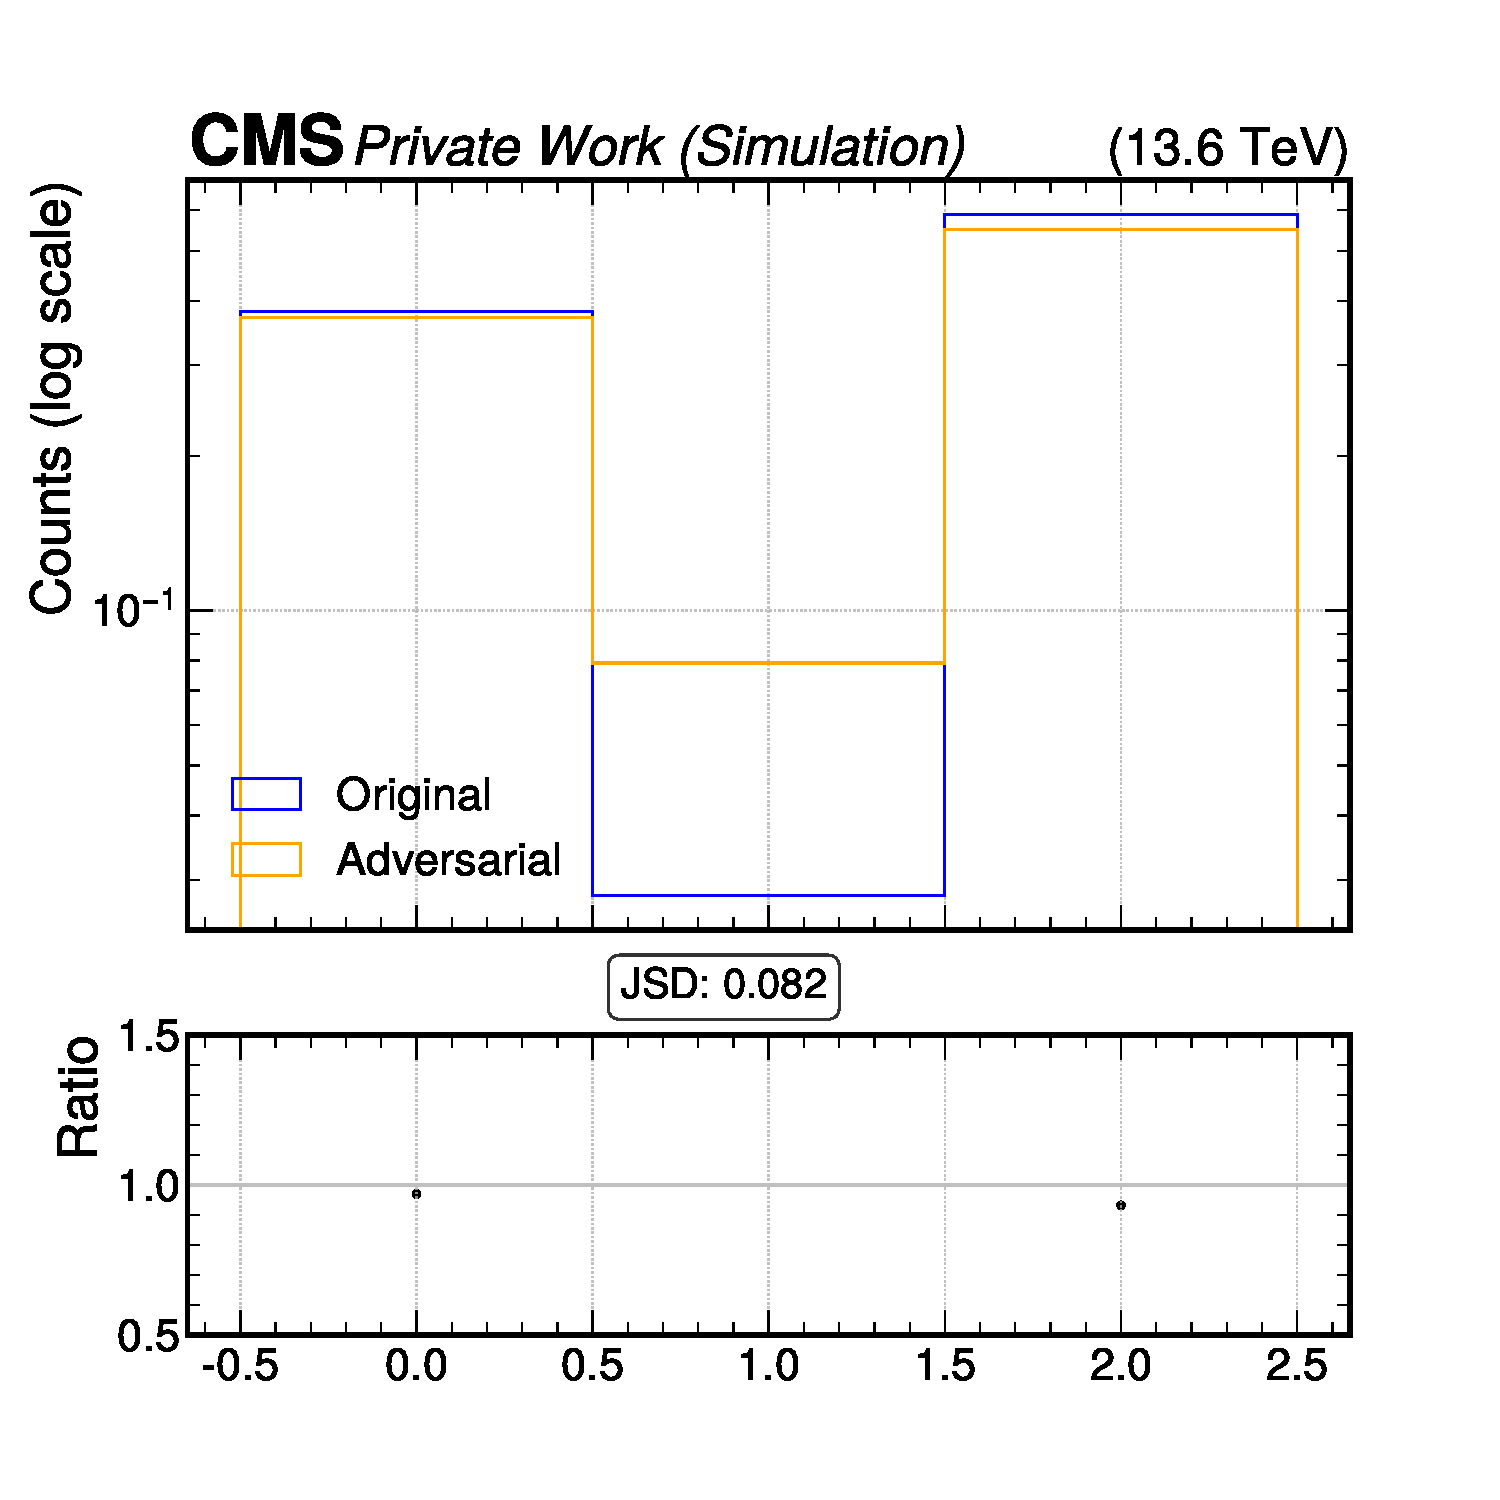
\includegraphics[width=\linewidth]{media/output/features/compare/intprob_2/cmp_global_features_TagVarCSV_vertexCategory.pdf}
    \caption{Input similarity for PIP(2).}
  \end{subfigure}\hfill
  \begin{subfigure}[t]{0.32\textwidth}
    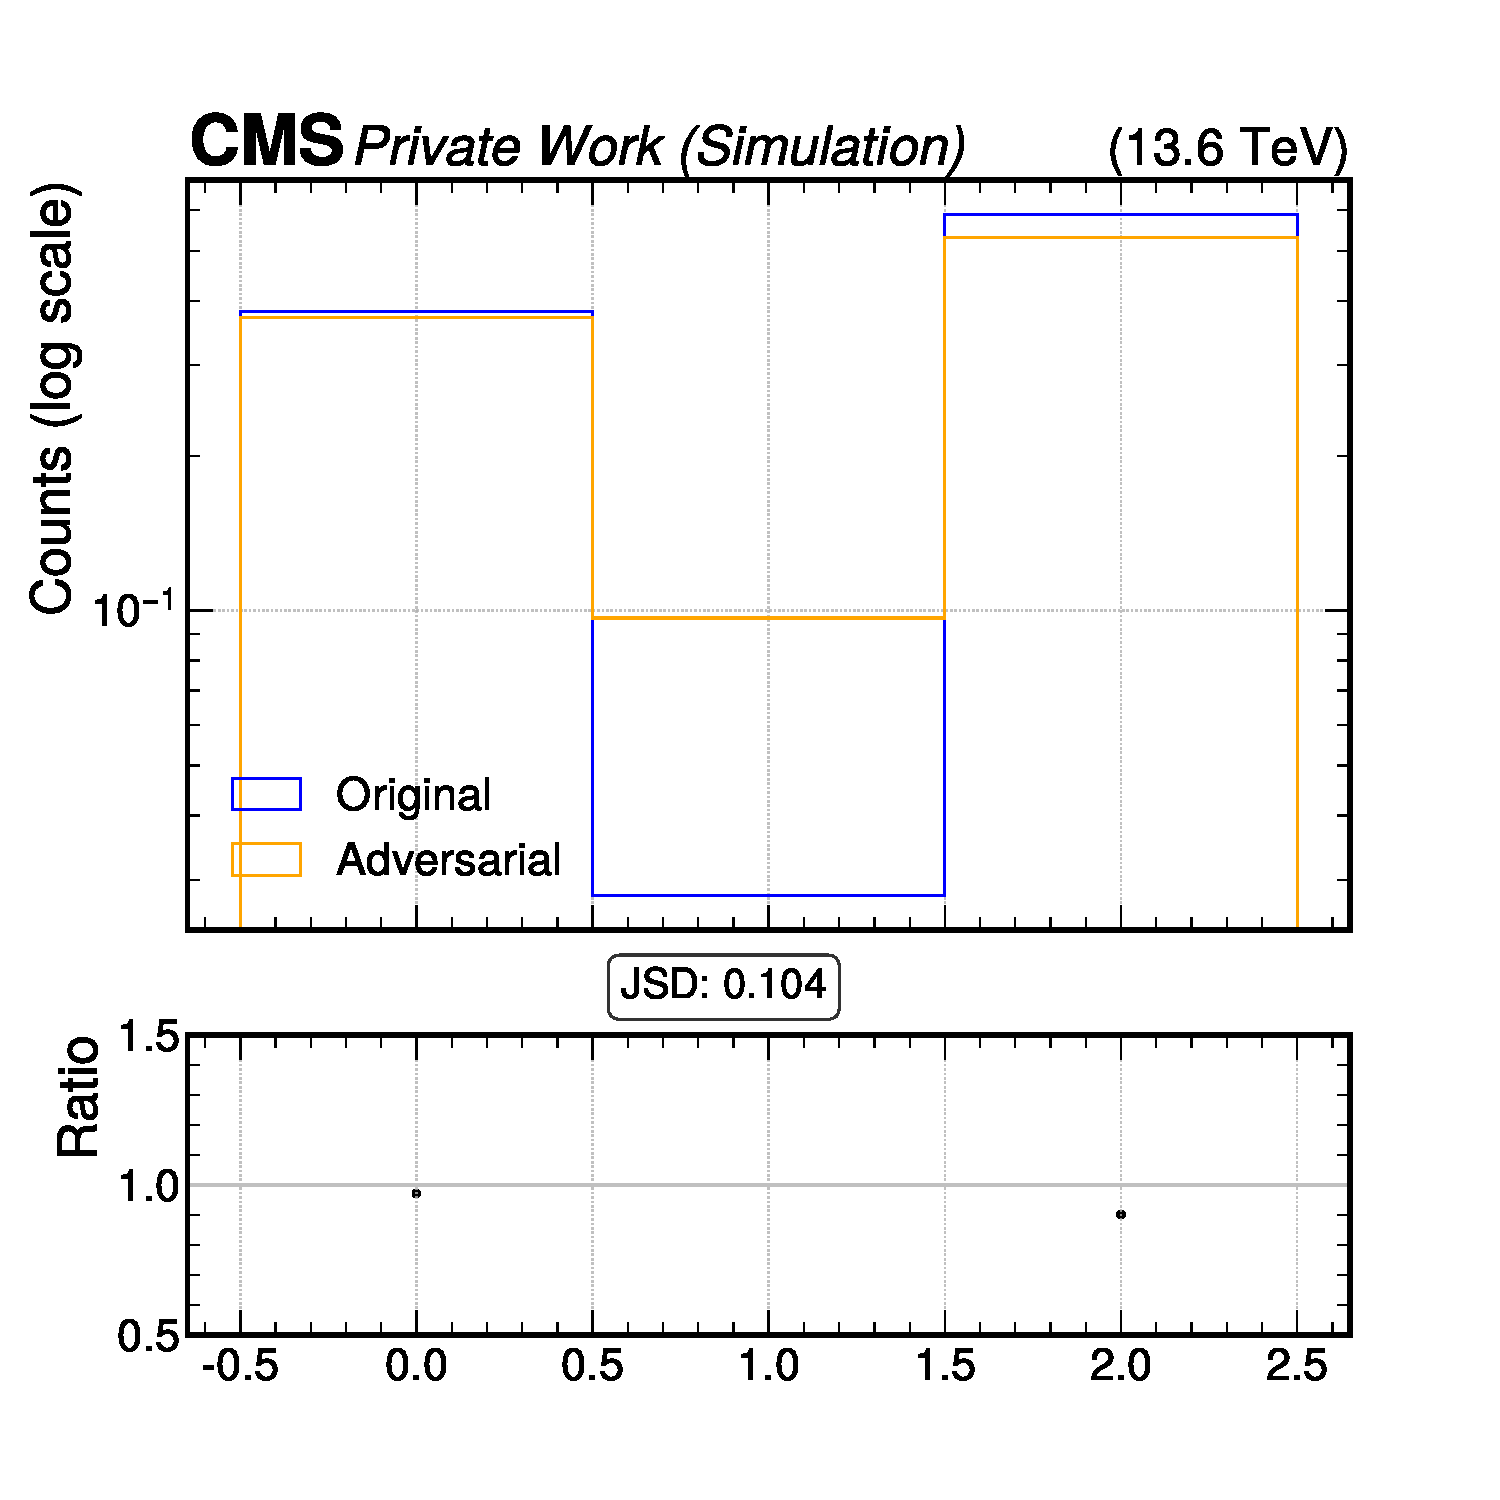
\includegraphics[width=\linewidth]{media/output/features/compare/intprob_3/cmp_global_features_TagVarCSV_vertexCategory.pdf}
    \caption{Input similarity for PIP(3).}
  \end{subfigure}

  \caption{Histogram of \texttt{TagVarCSV\_vertexCategory} for multiple iterations of PIP tested against nominal inputs.}
  \label{fig:intprob_input_TagVarCSV_vertexCategory}
\end{figure}

\FloatBarrier
\newpage
\subsection*{CPF Features}

\begin{figure}[h]
  \centering
  \begin{subfigure}[t]{0.32\textwidth}
    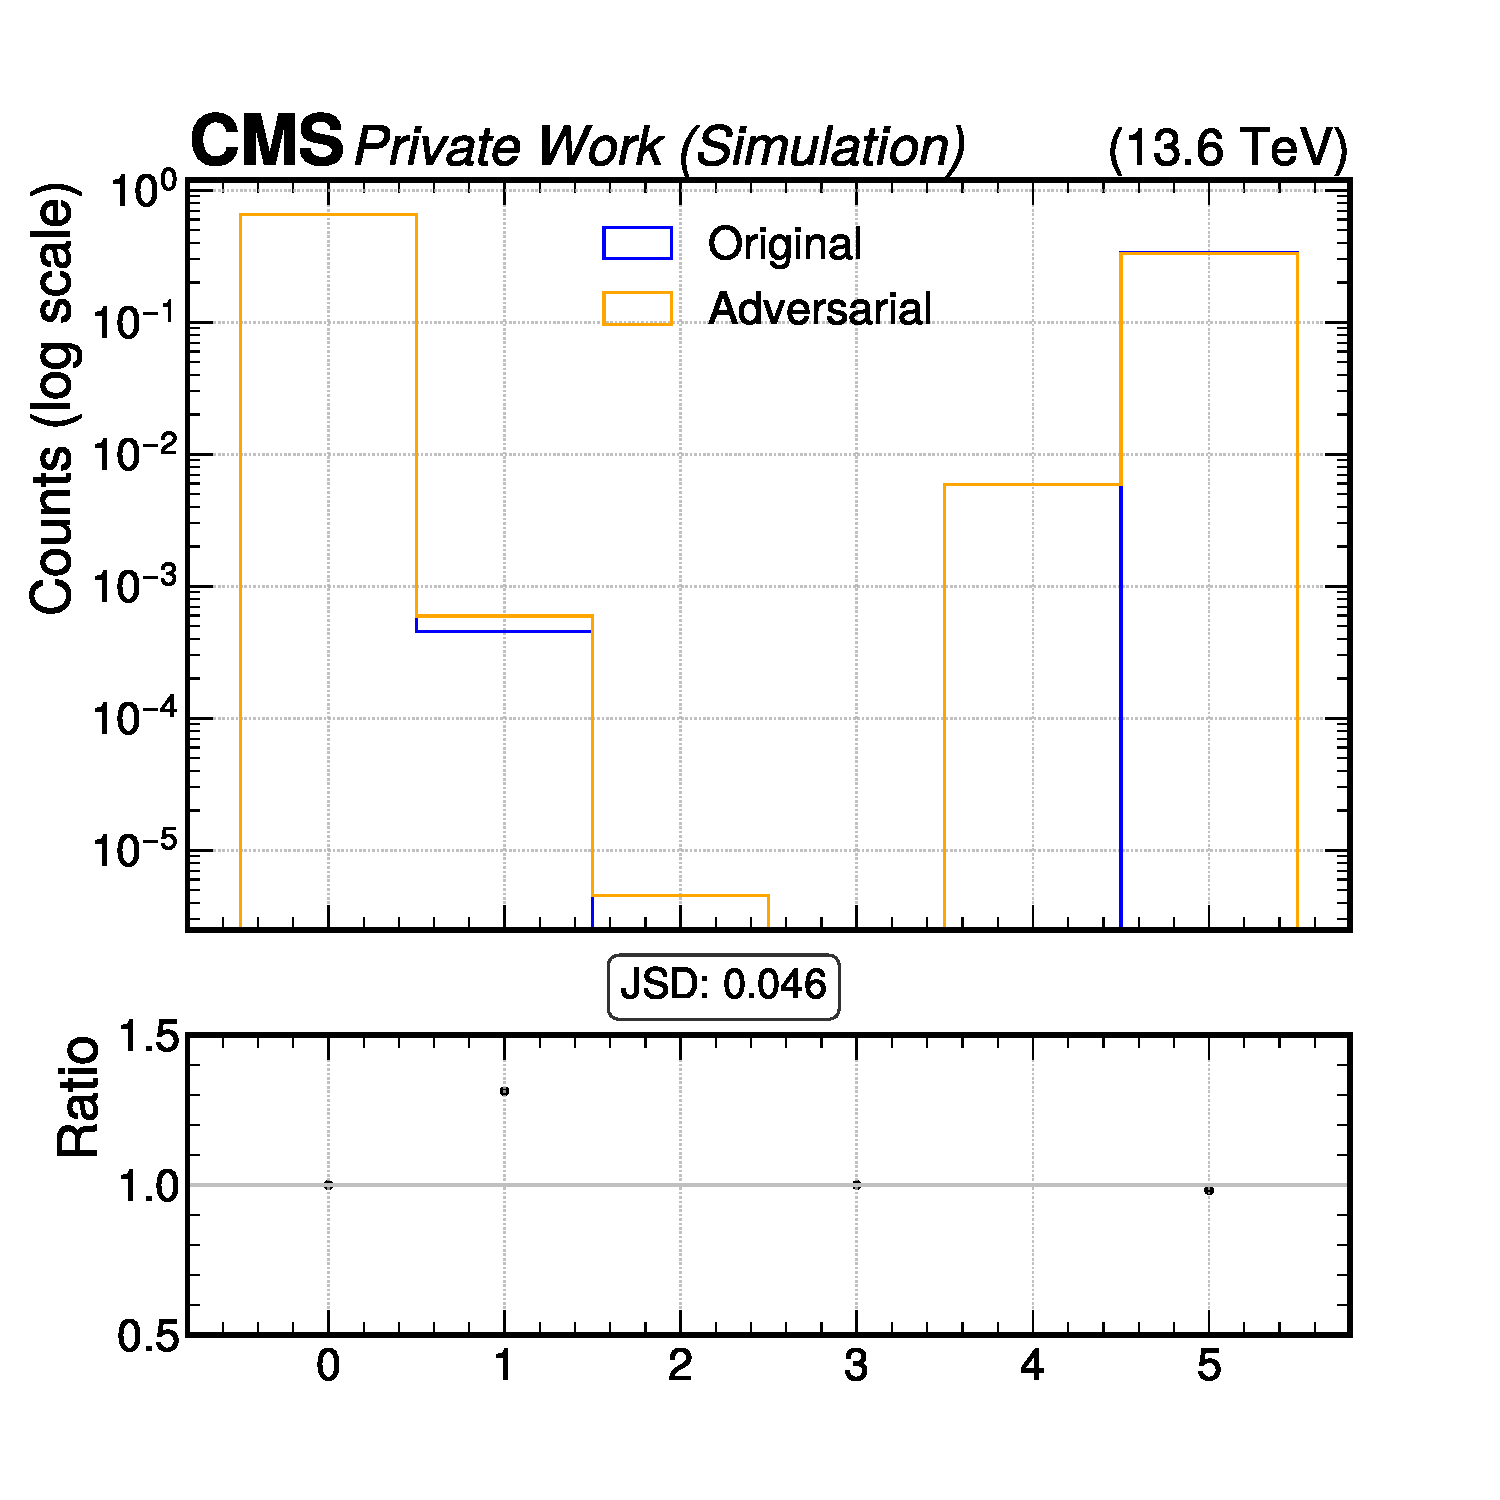
\includegraphics[width=\linewidth]{media/output/features/compare/intprob_1/cmp_cpf_arr_Cpfcan_quality.pdf}
    \caption{Input similarity for PIP(1).}
  \end{subfigure}\hfill
  \begin{subfigure}[t]{0.32\textwidth}
    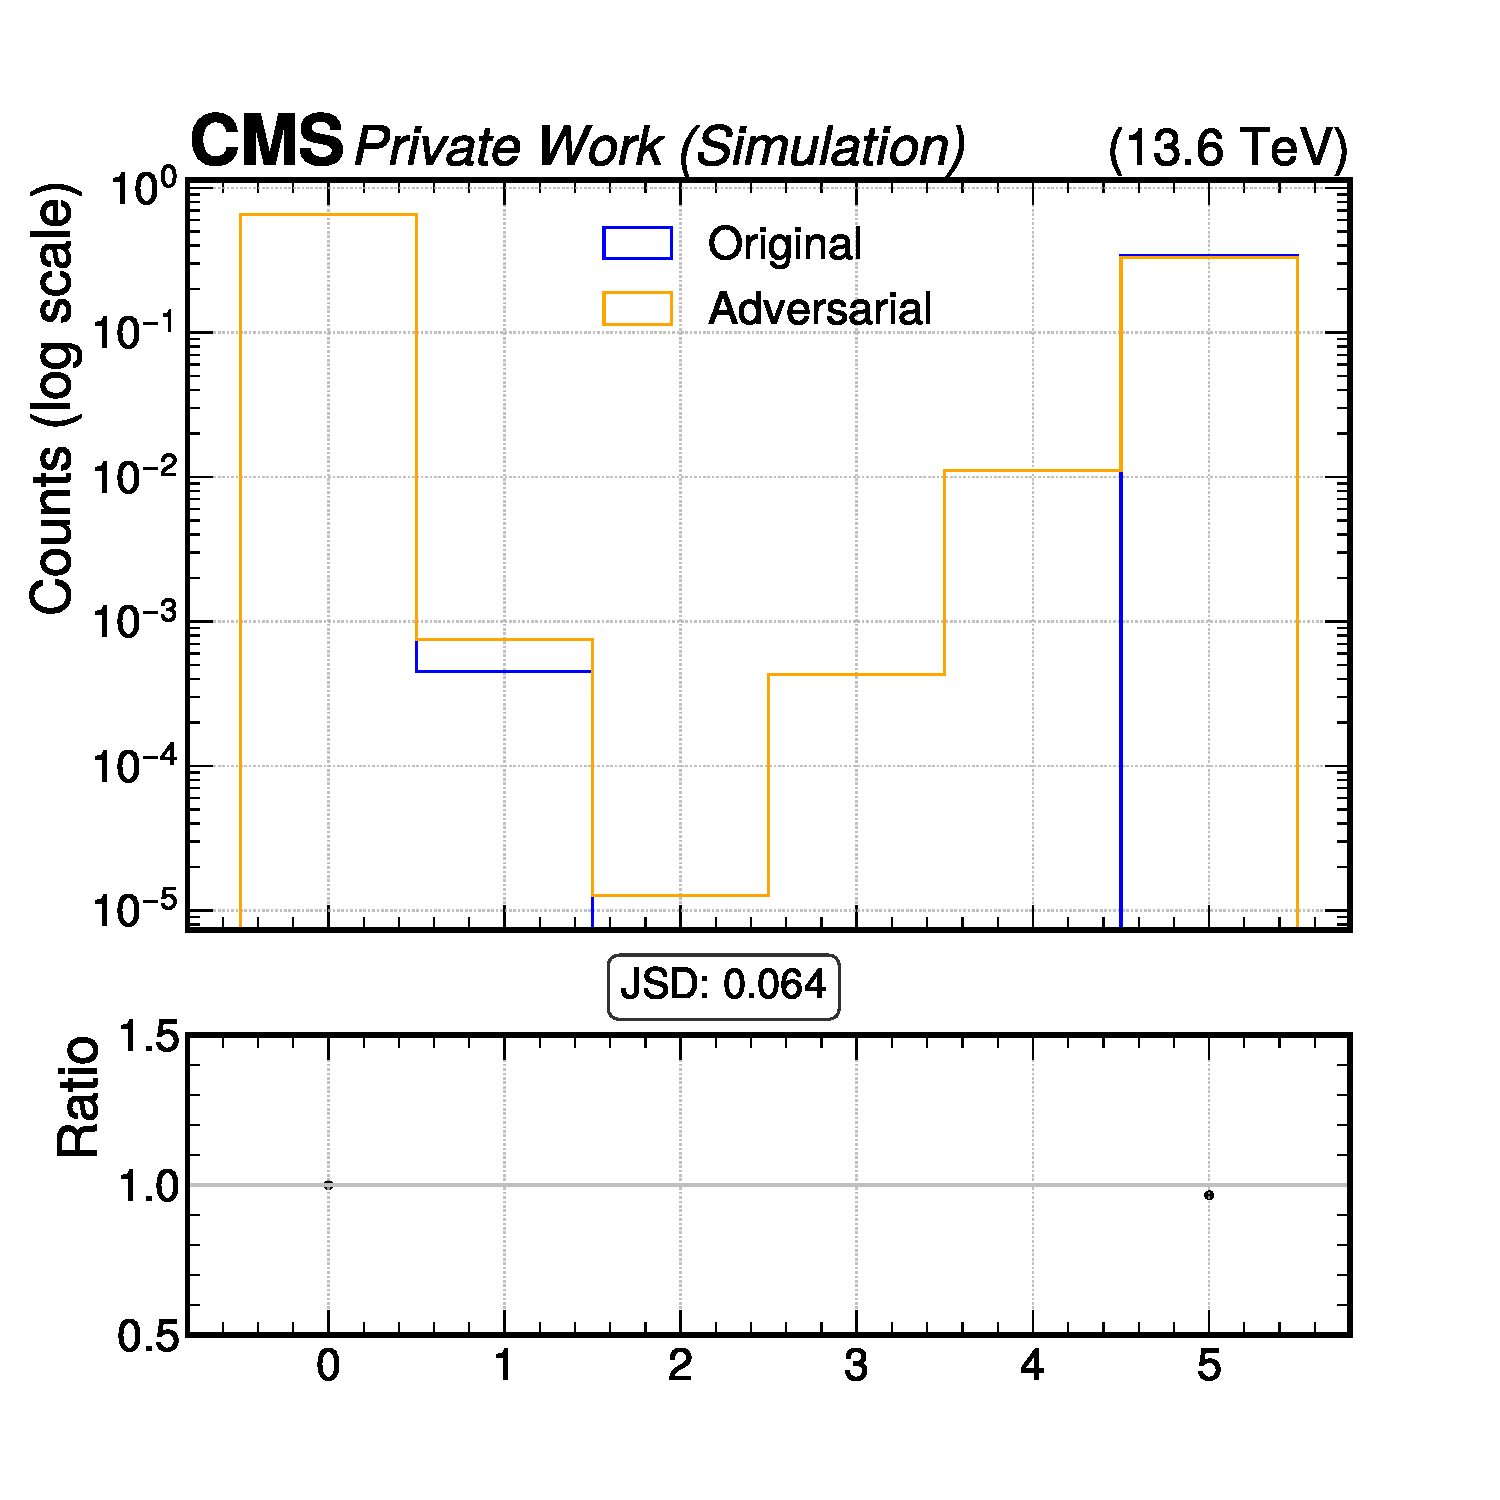
\includegraphics[width=\linewidth]{media/output/features/compare/intprob_2/cmp_cpf_arr_Cpfcan_quality.pdf}
    \caption{Input similarity for PIP(2).}
  \end{subfigure}\hfill
  \begin{subfigure}[t]{0.32\textwidth}
    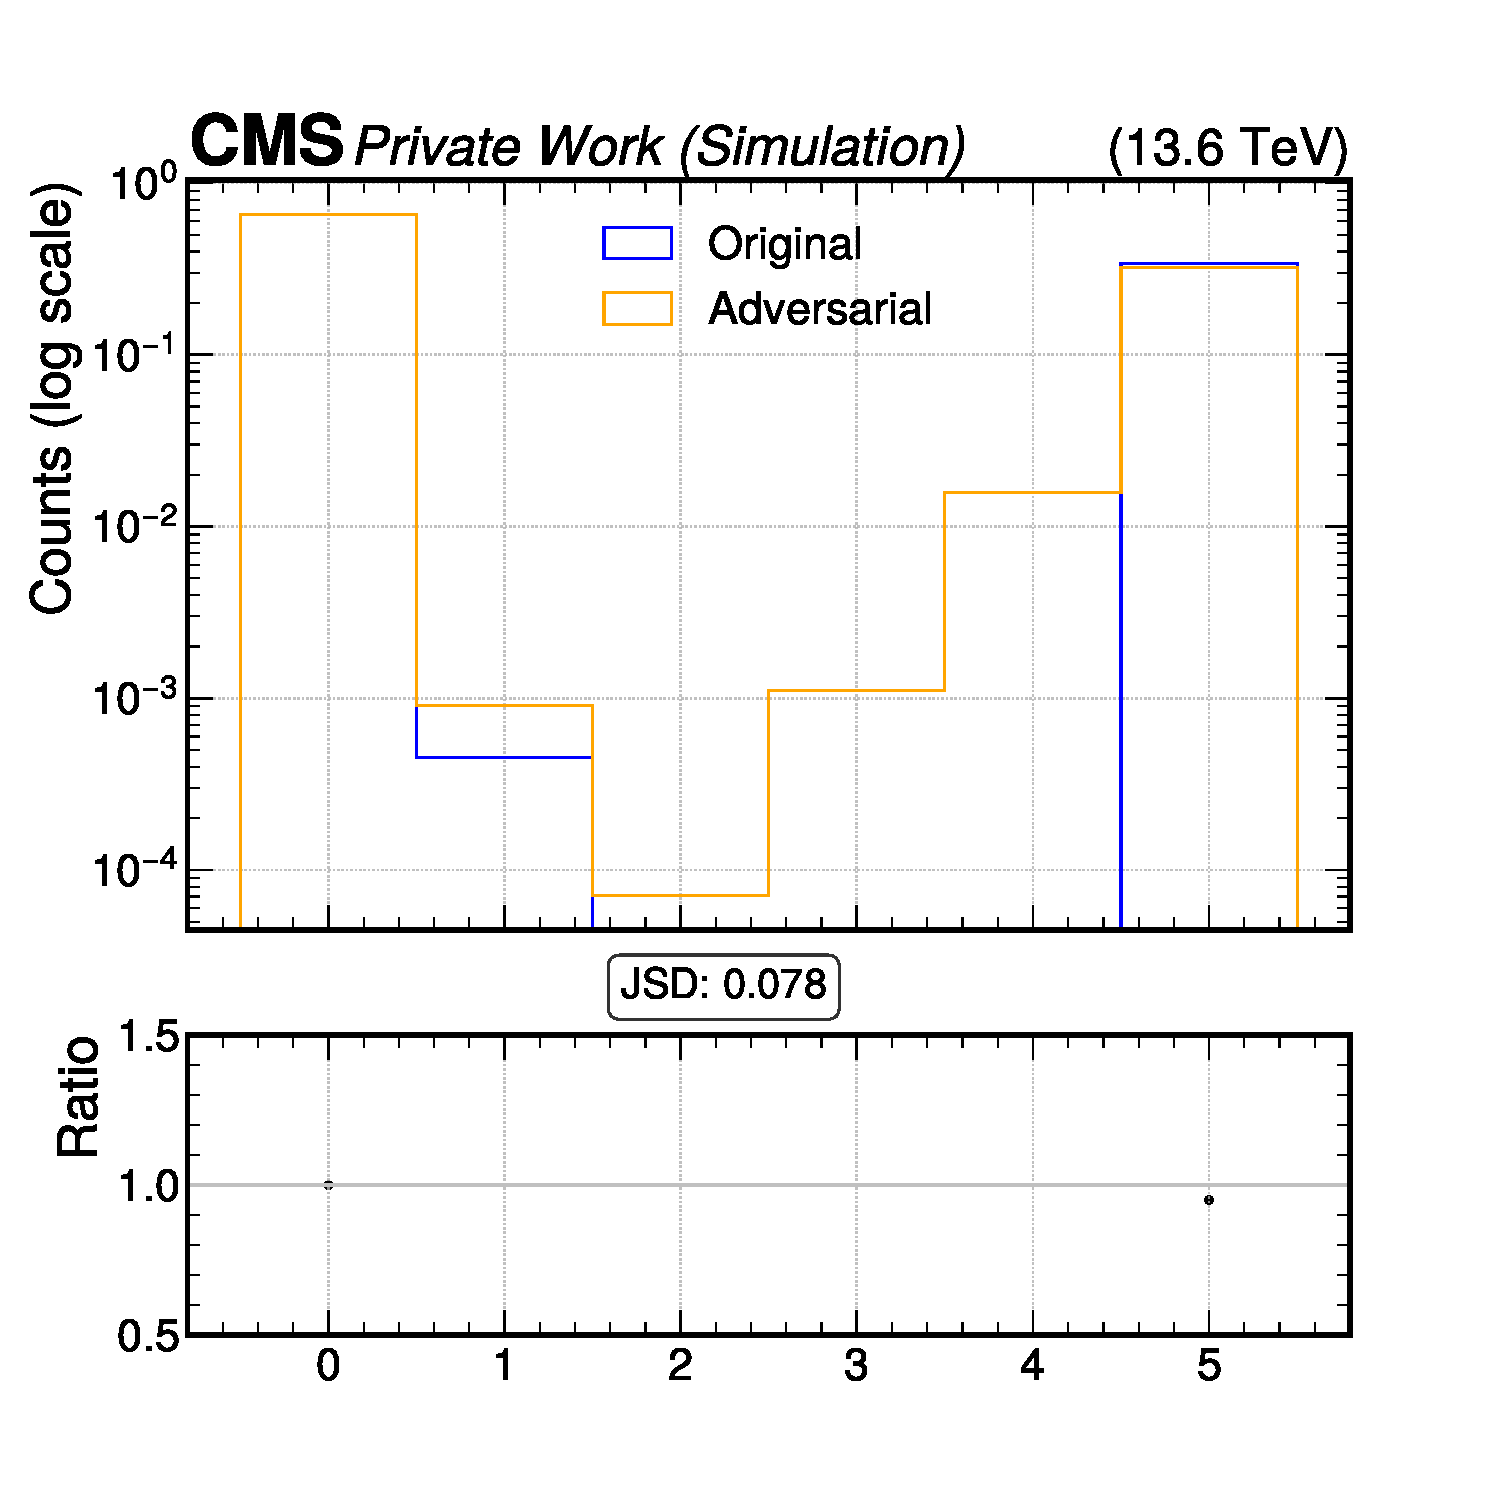
\includegraphics[width=\linewidth]{media/output/features/compare/intprob_3/cmp_cpf_arr_Cpfcan_quality.pdf}
    \caption{Input similarity for PIP(3).}
  \end{subfigure}

  \caption{Histogram of \texttt{Cpfcan\_quality} for multiple iterations of PIP tested against nominal inputs.}
  \label{fig:intprob_input_Cpfcan_quality}
\end{figure}
\begin{figure}[h]
  \centering
  \begin{subfigure}[t]{0.32\textwidth}
    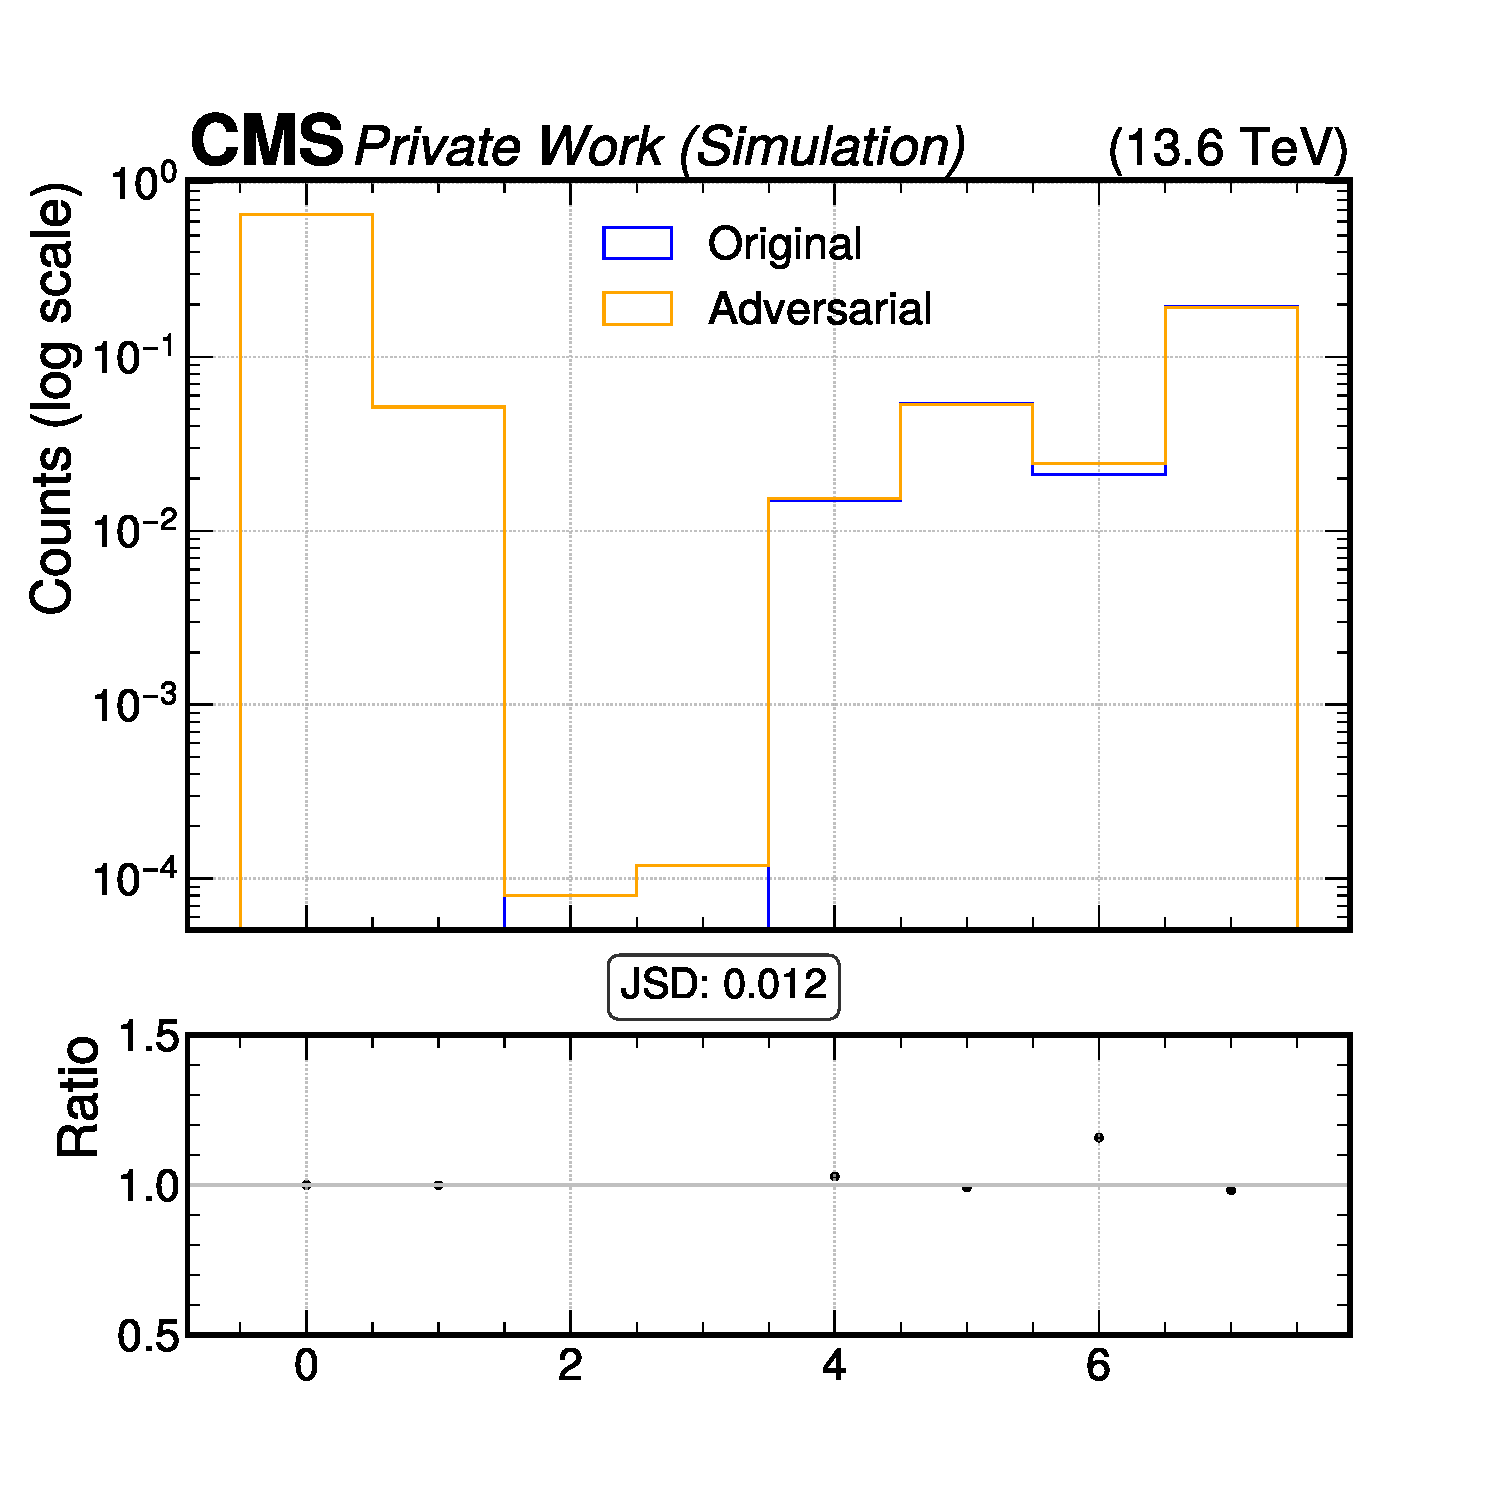
\includegraphics[width=\linewidth]{media/output/features/compare/intprob_1/cmp_cpf_arr_Cpfcan_VTX_ass.pdf}
    \caption{Input similarity for PIP(1).}
  \end{subfigure}\hfill
  \begin{subfigure}[t]{0.32\textwidth}
    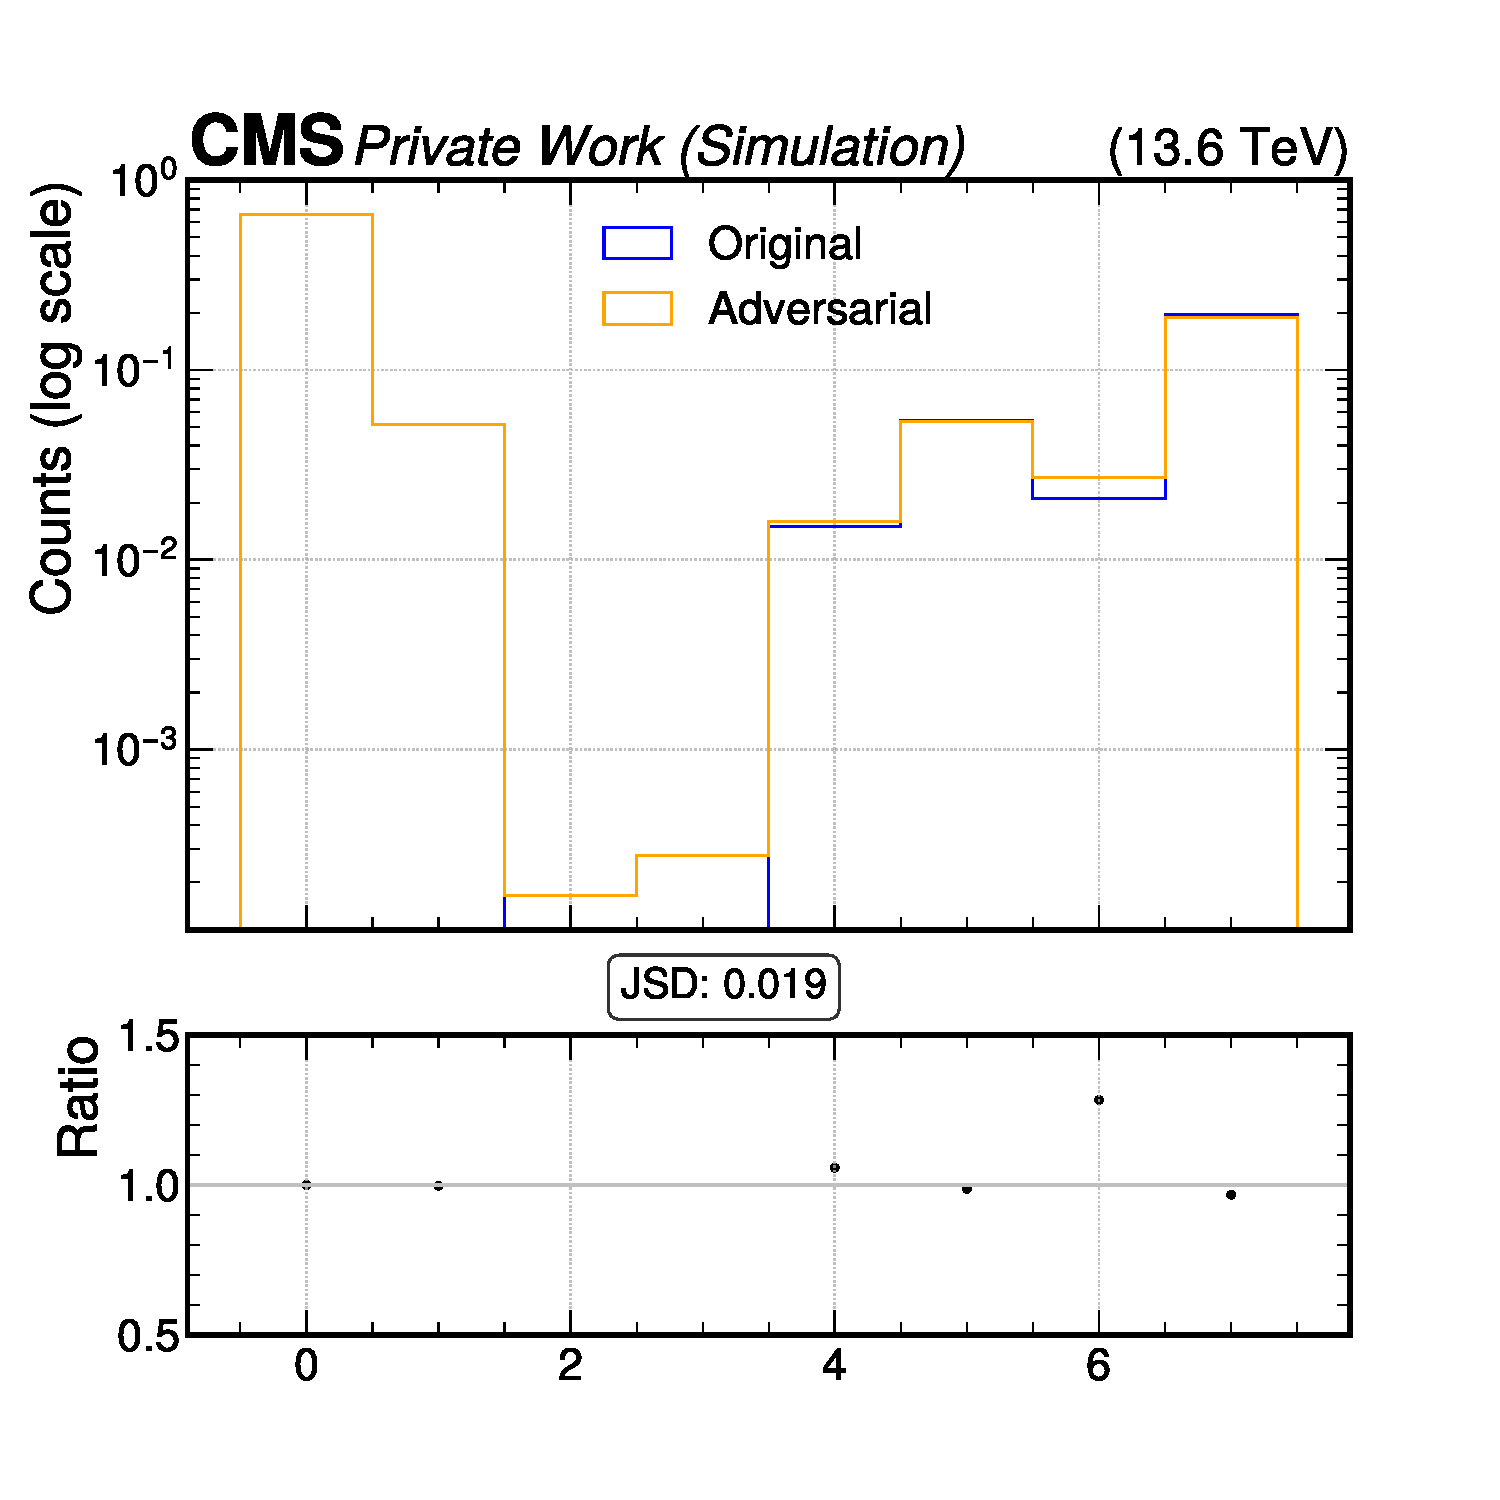
\includegraphics[width=\linewidth]{media/output/features/compare/intprob_2/cmp_cpf_arr_Cpfcan_VTX_ass.pdf}
    \caption{Input similarity for PIP(2).}
  \end{subfigure}\hfill
  \begin{subfigure}[t]{0.32\textwidth}
    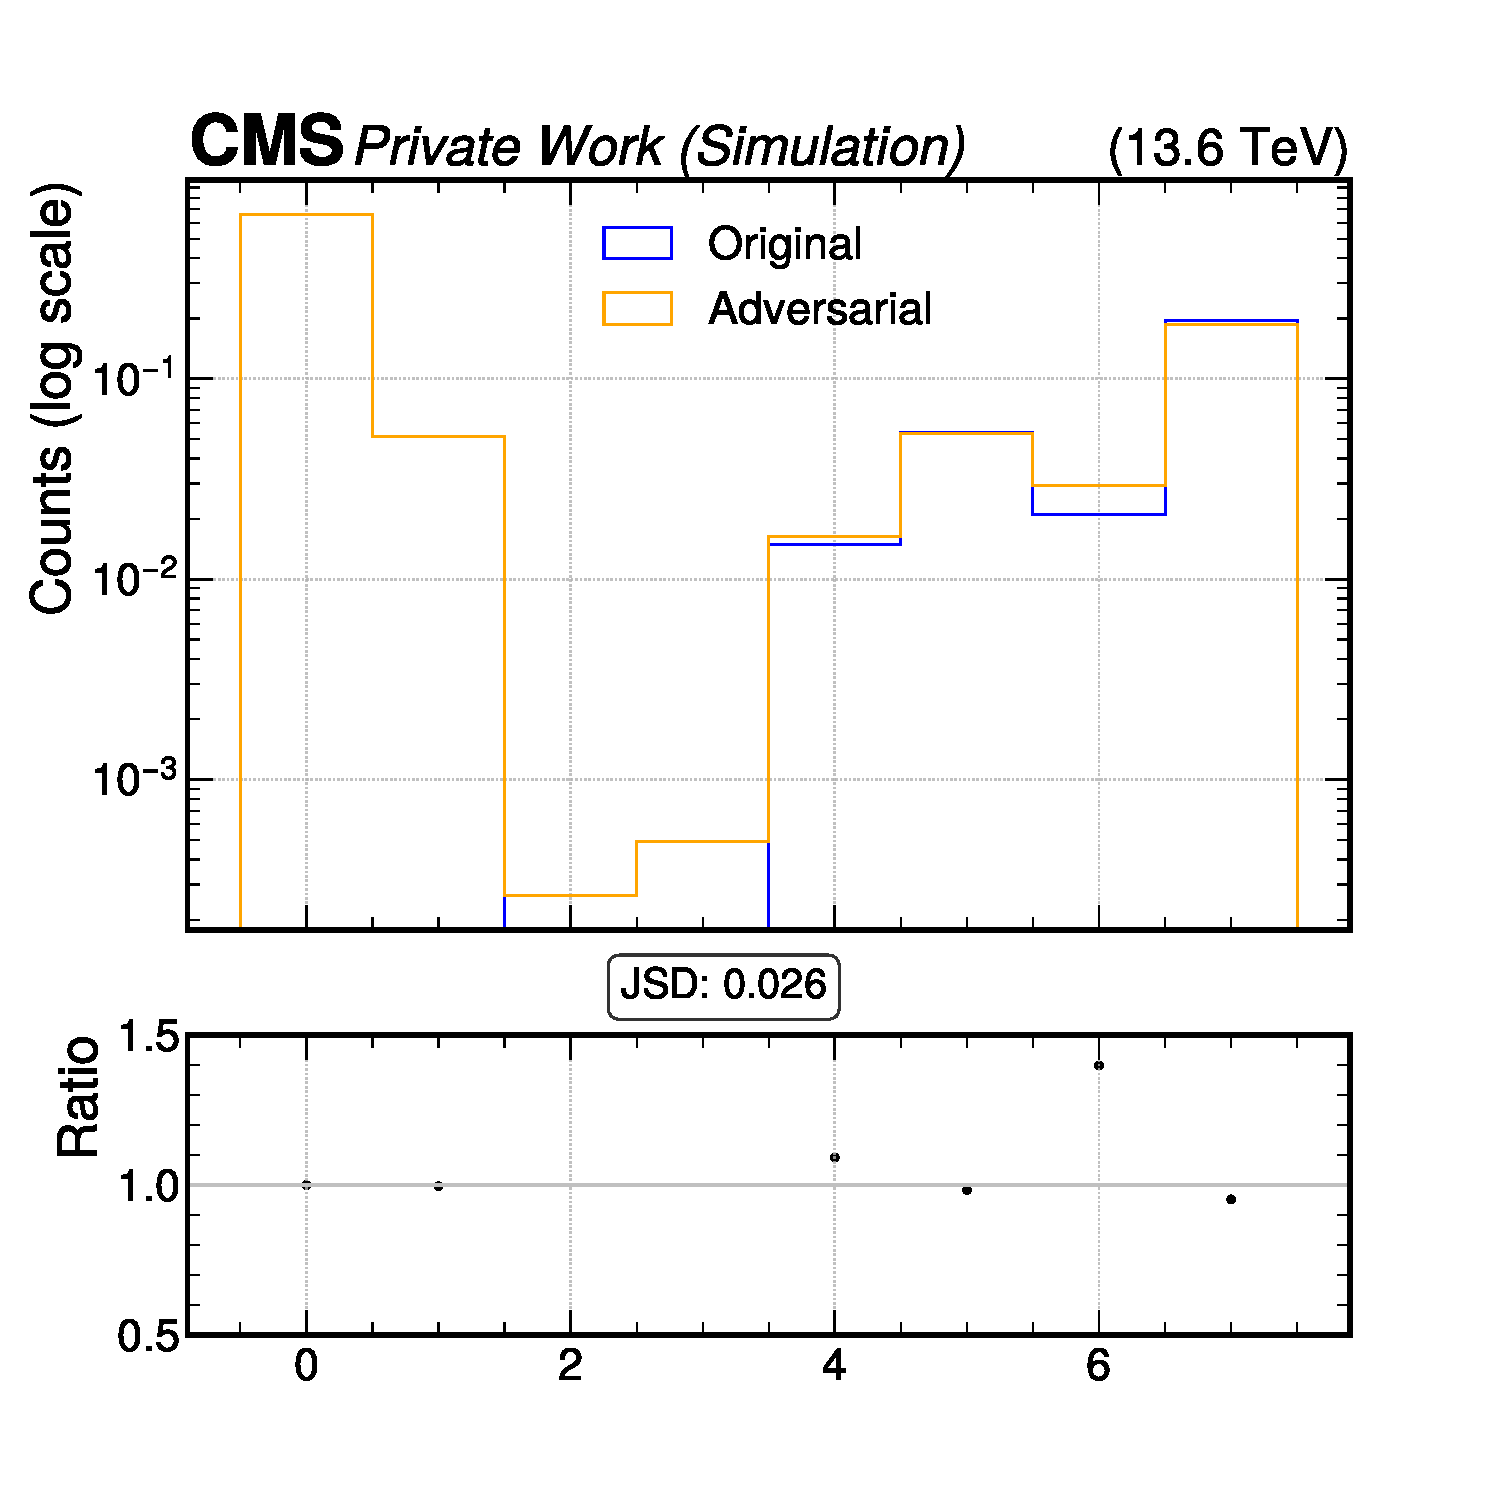
\includegraphics[width=\linewidth]{media/output/features/compare/intprob_3/cmp_cpf_arr_Cpfcan_VTX_ass.pdf}
    \caption{Input similarity for PIP(3).}
  \end{subfigure}

  \caption{Histogram of \texttt{Cpfcan\_VTX\_ass} for multiple iterations of PIP tested against nominal inputs.}
  \label{fig:intprob_input_Cpfcan_VTX_ass}
\end{figure}

\newpage
\subsection*{NPF Features}

\begin{figure}[h]
  \centering
  \begin{subfigure}[t]{0.32\textwidth}
    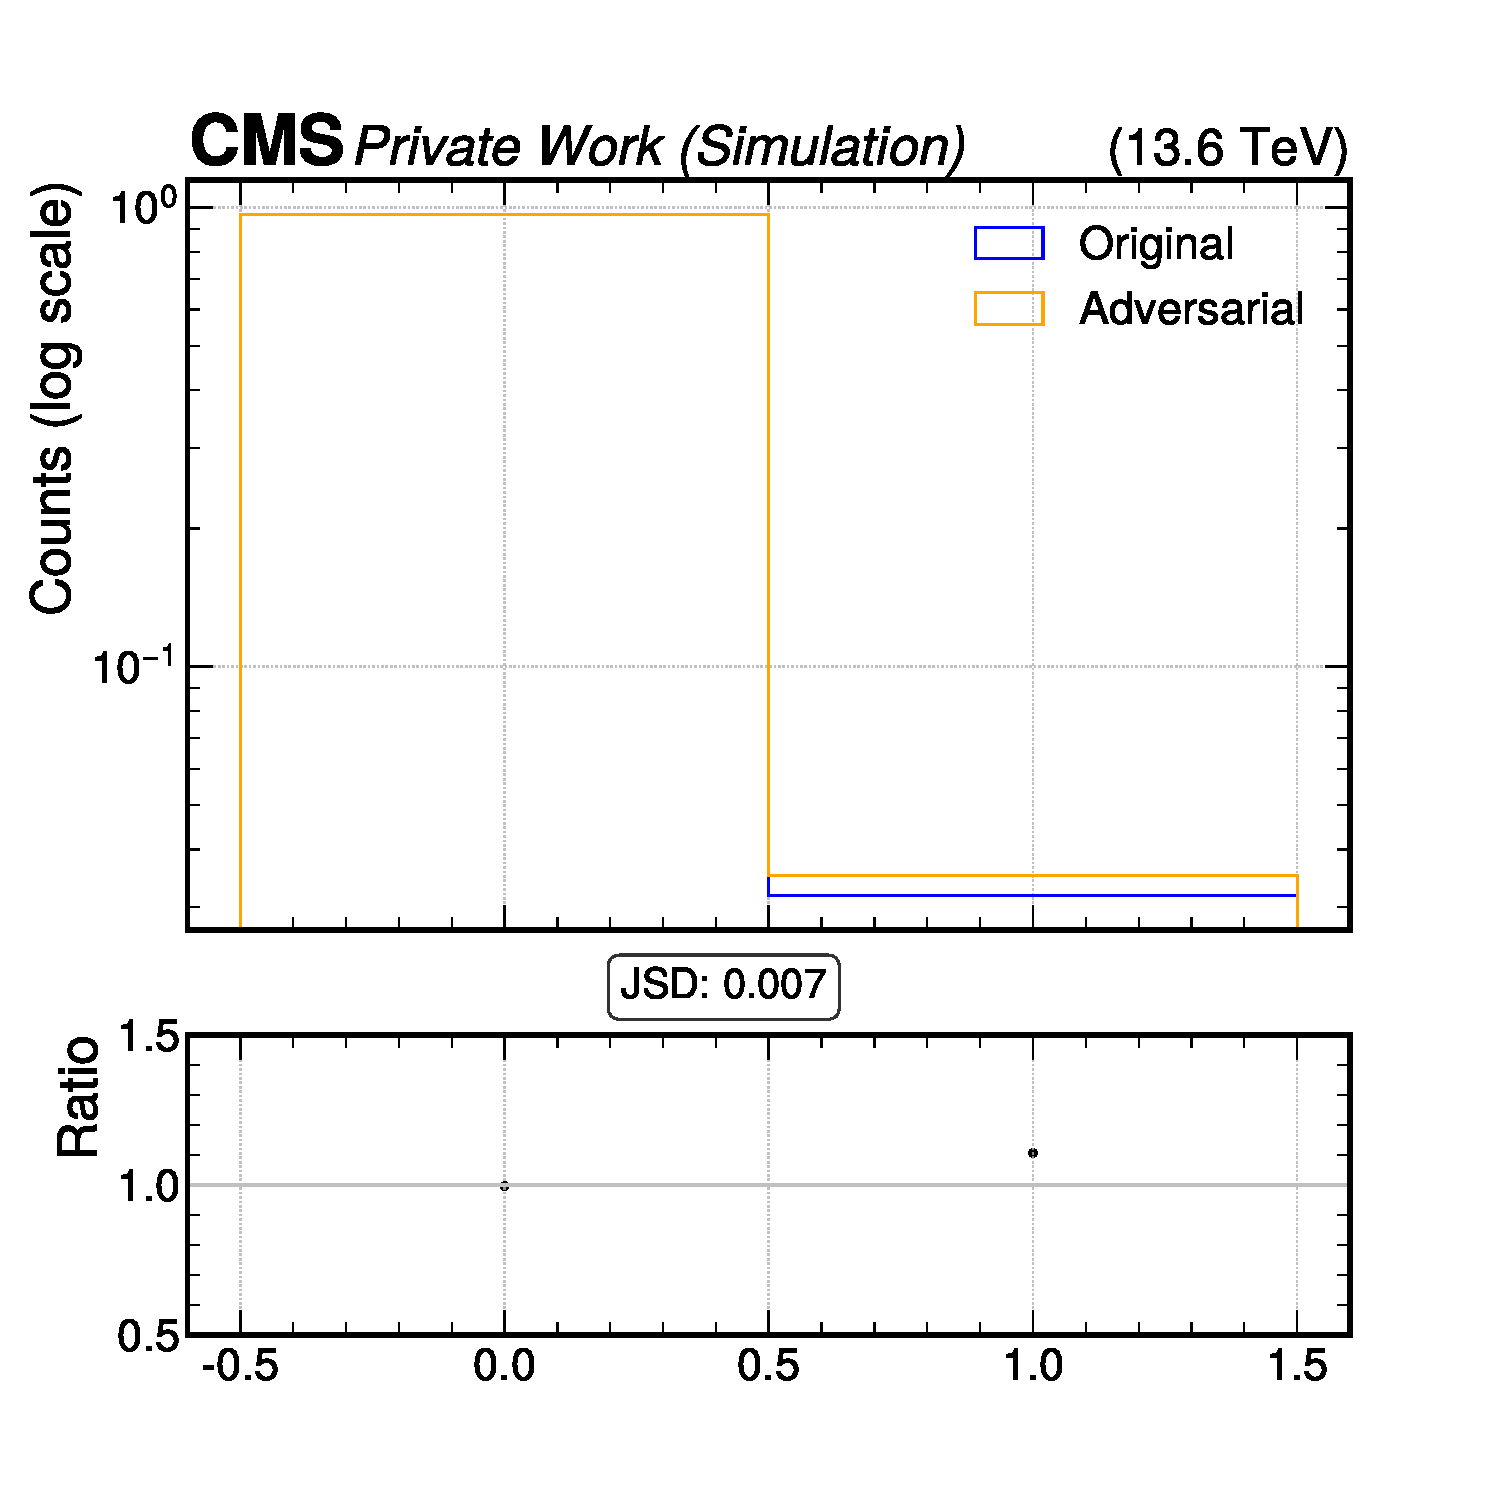
\includegraphics[width=\linewidth]{media/output/features/compare/intprob_1/cmp_npf_arr_Npfcan_HadFrac.pdf}
    \caption{Input similarity for PIP(1).}
  \end{subfigure}\hfill
  \begin{subfigure}[t]{0.32\textwidth}
    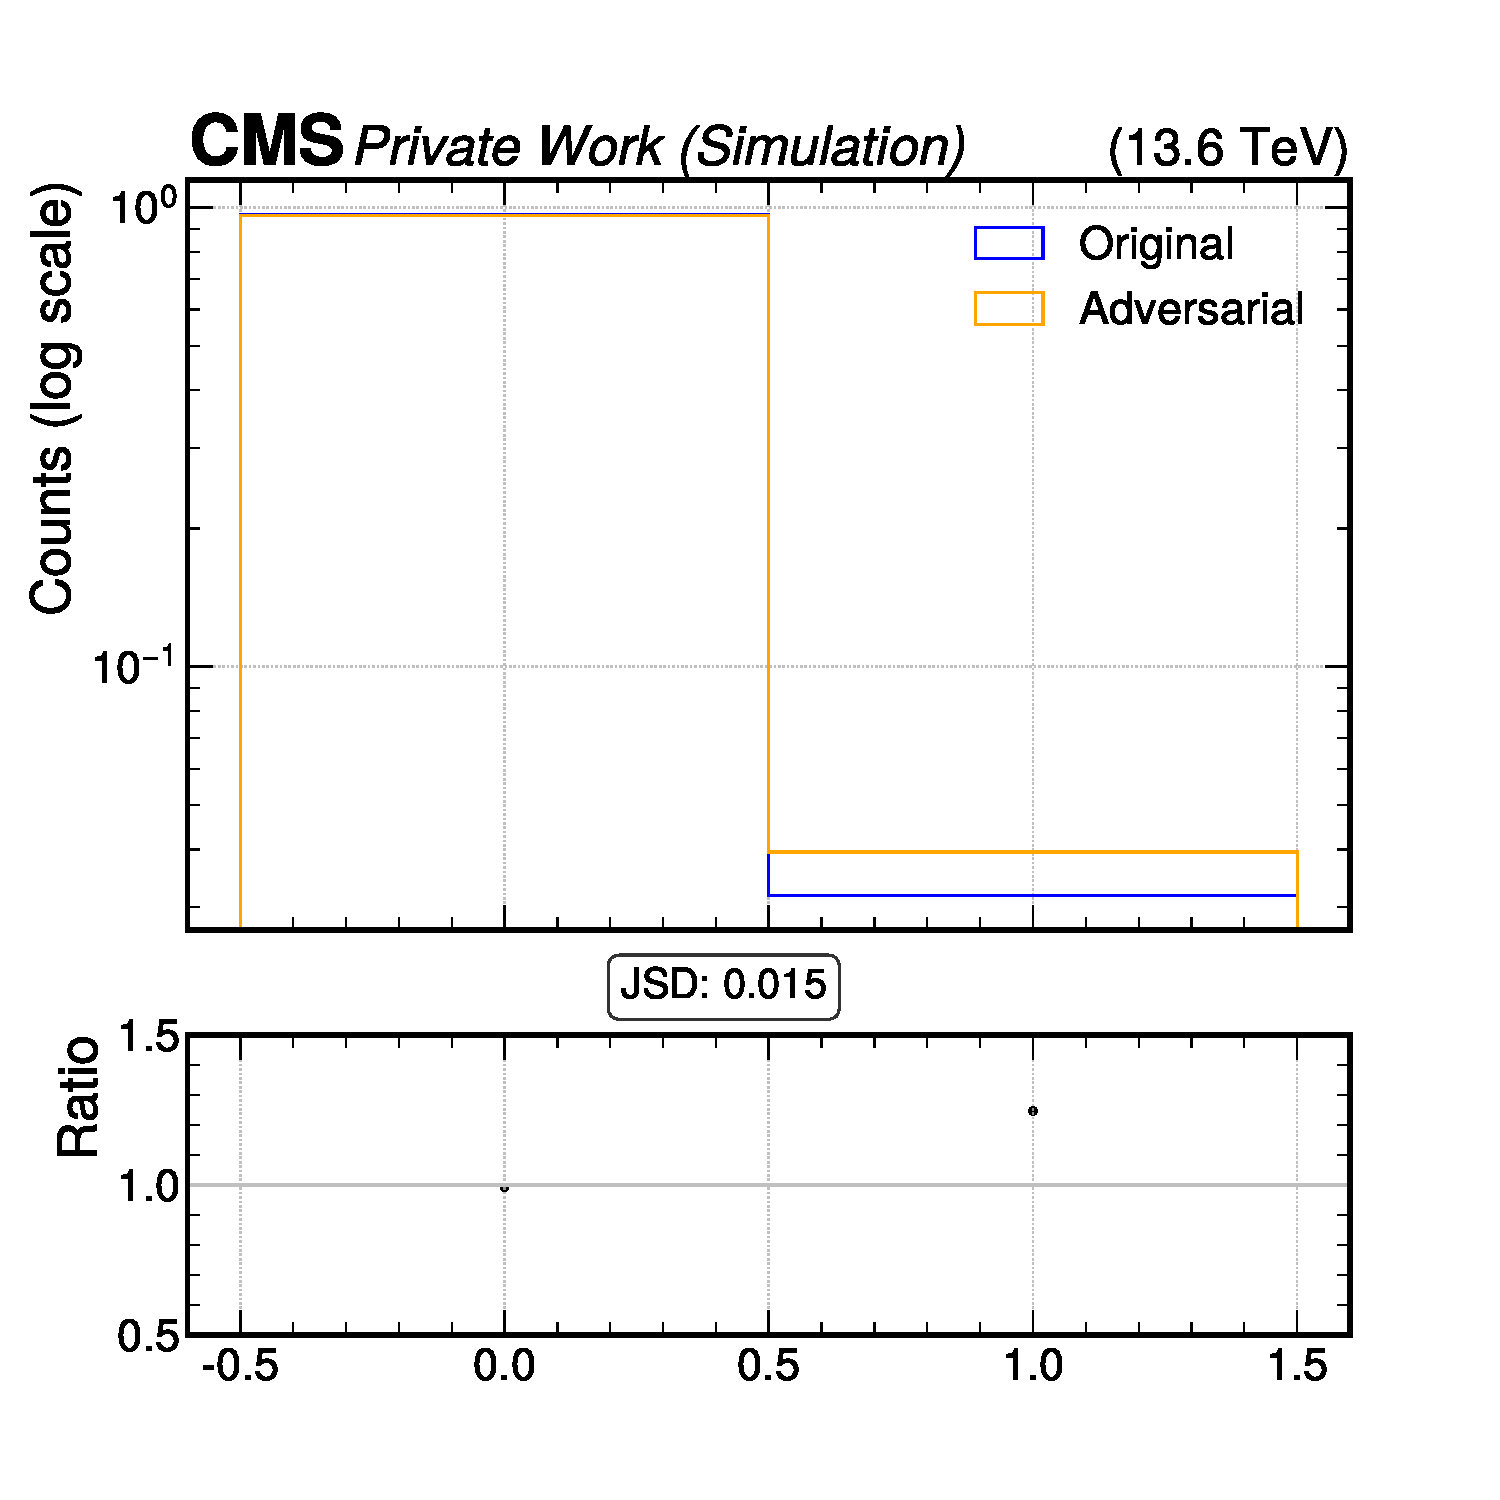
\includegraphics[width=\linewidth]{media/output/features/compare/intprob_2/cmp_npf_arr_Npfcan_HadFrac.pdf}
    \caption{Input similarity for PIP(2).}
  \end{subfigure}\hfill
  \begin{subfigure}[t]{0.32\textwidth}
    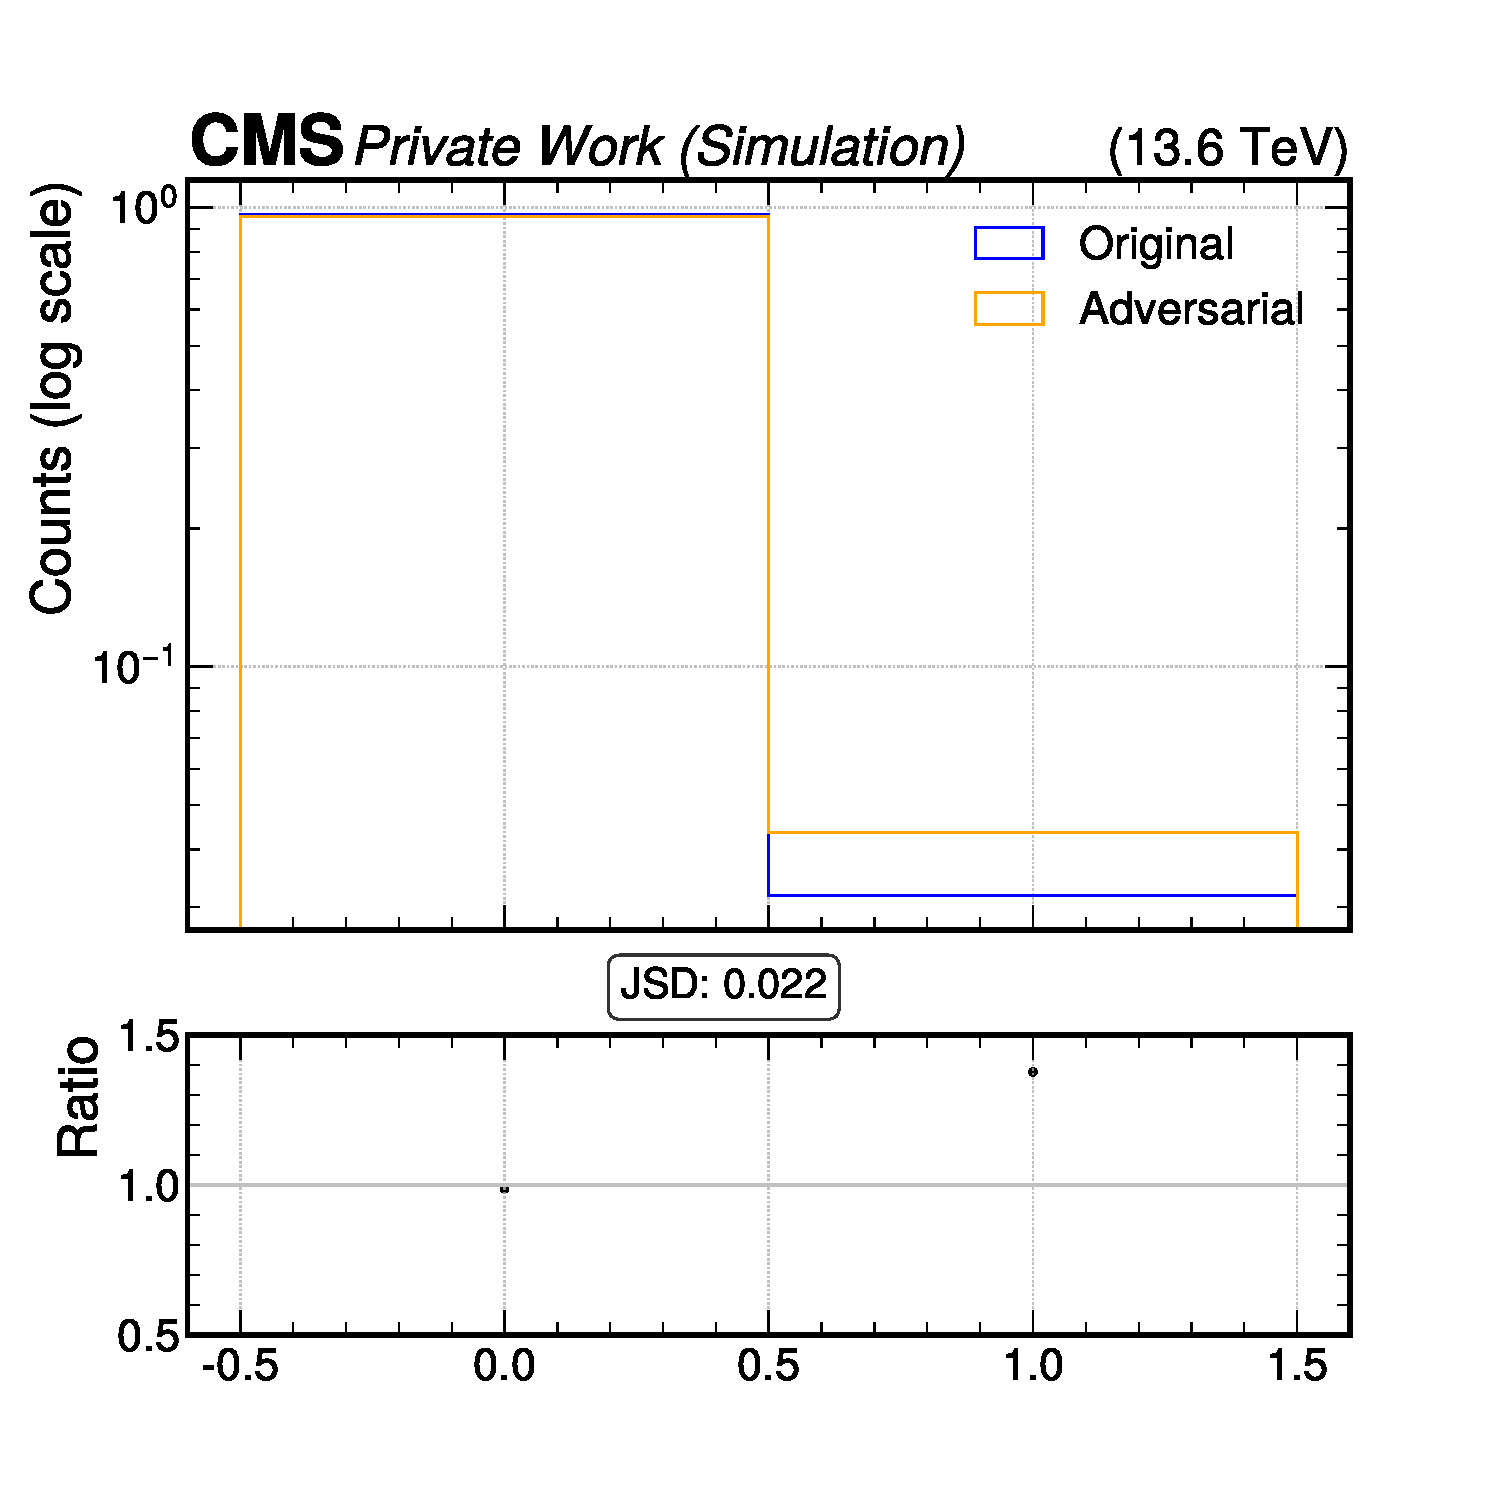
\includegraphics[width=\linewidth]{media/output/features/compare/intprob_3/cmp_npf_arr_Npfcan_HadFrac.pdf}
    \caption{Input similarity for PIP(3).}
  \end{subfigure}

  \caption{Histogram of \texttt{Npfcan\_HadFrac} for multiple iterations of PIP tested against nominal inputs.}
  \label{fig:intprob_input_Npfcan_HadFrac}
\end{figure}
\begin{figure}[h]
  \centering
  \begin{subfigure}[t]{0.32\textwidth}
    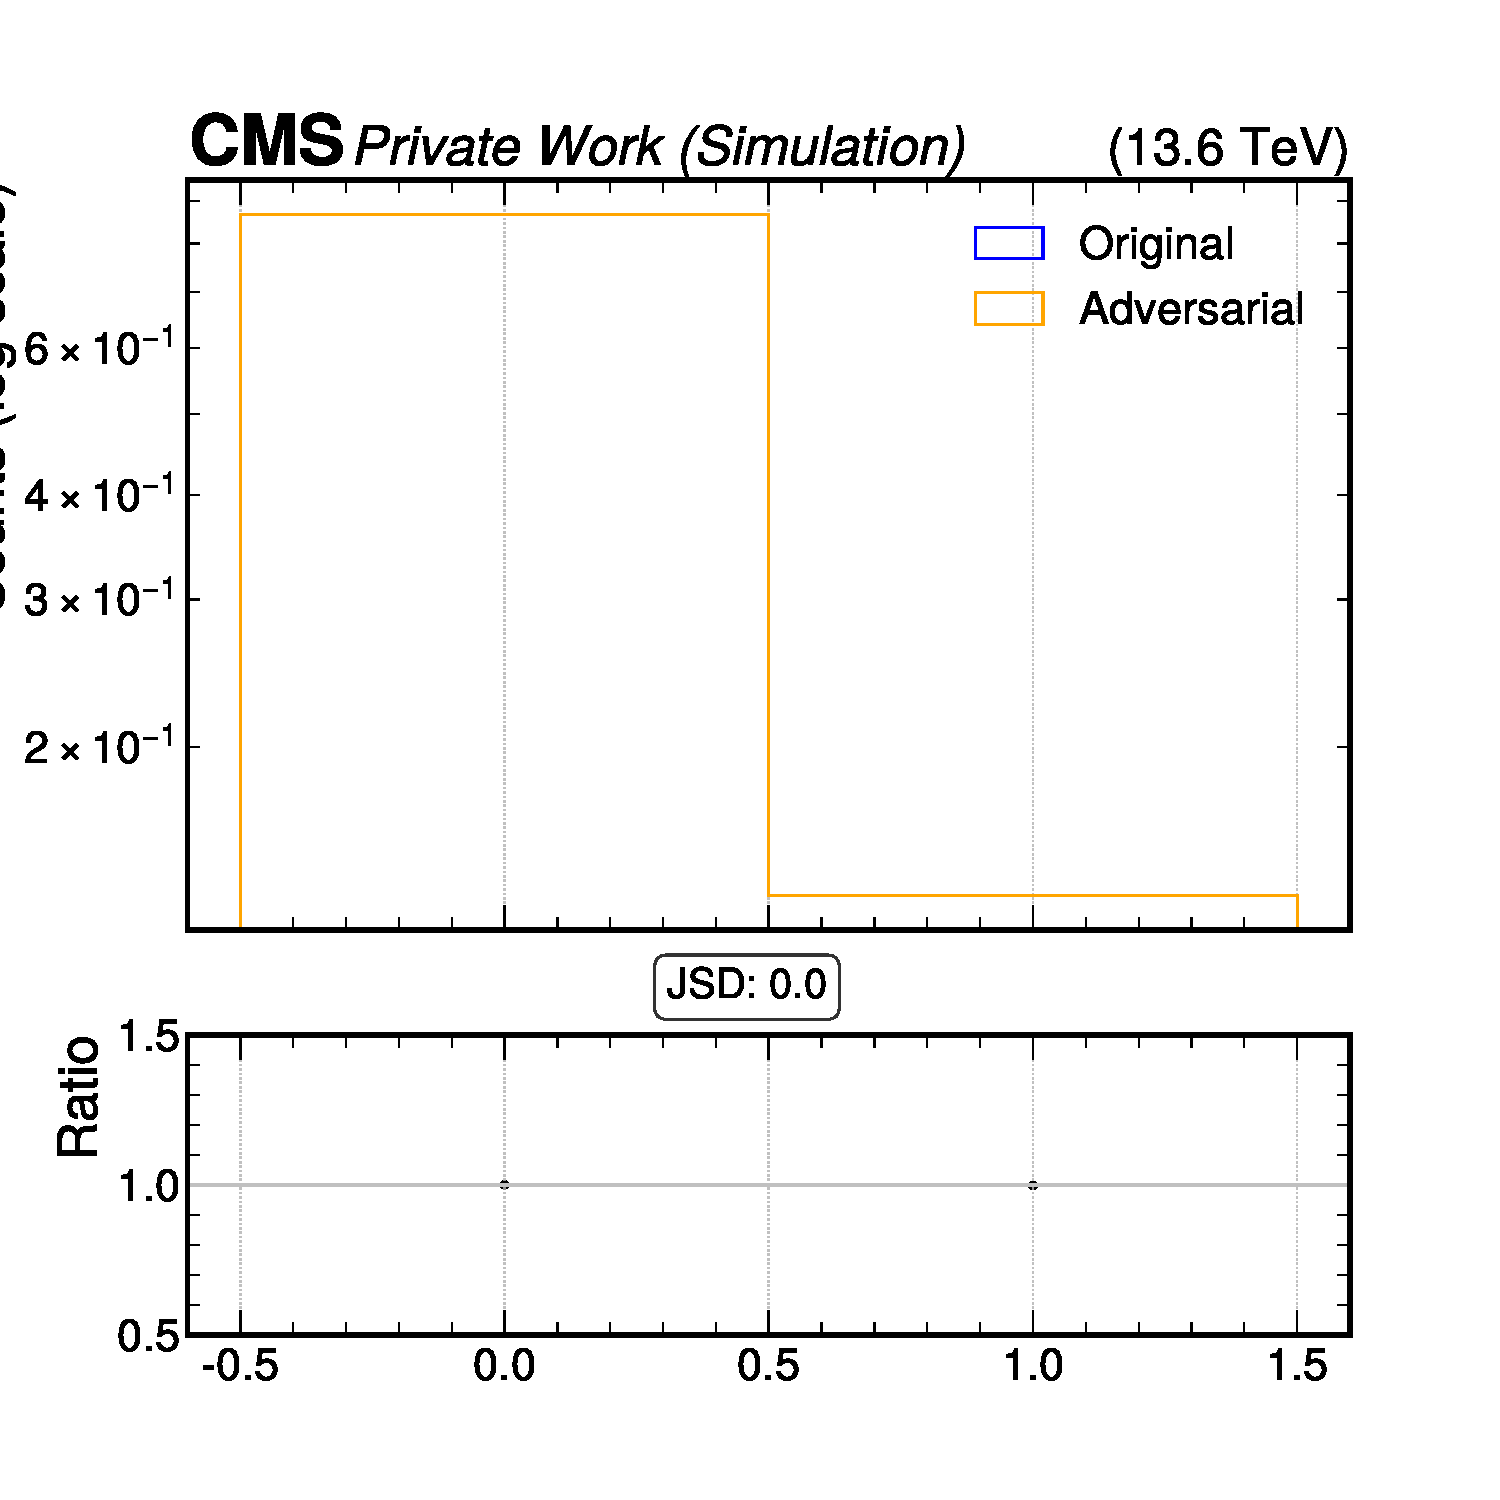
\includegraphics[width=\linewidth]{media/output/features/compare/intprob_1/cmp_npf_arr_Npfcan_isGamma.pdf}
    \caption{Input similarity for PIP(1).}
  \end{subfigure}\hfill
  \begin{subfigure}[t]{0.32\textwidth}
    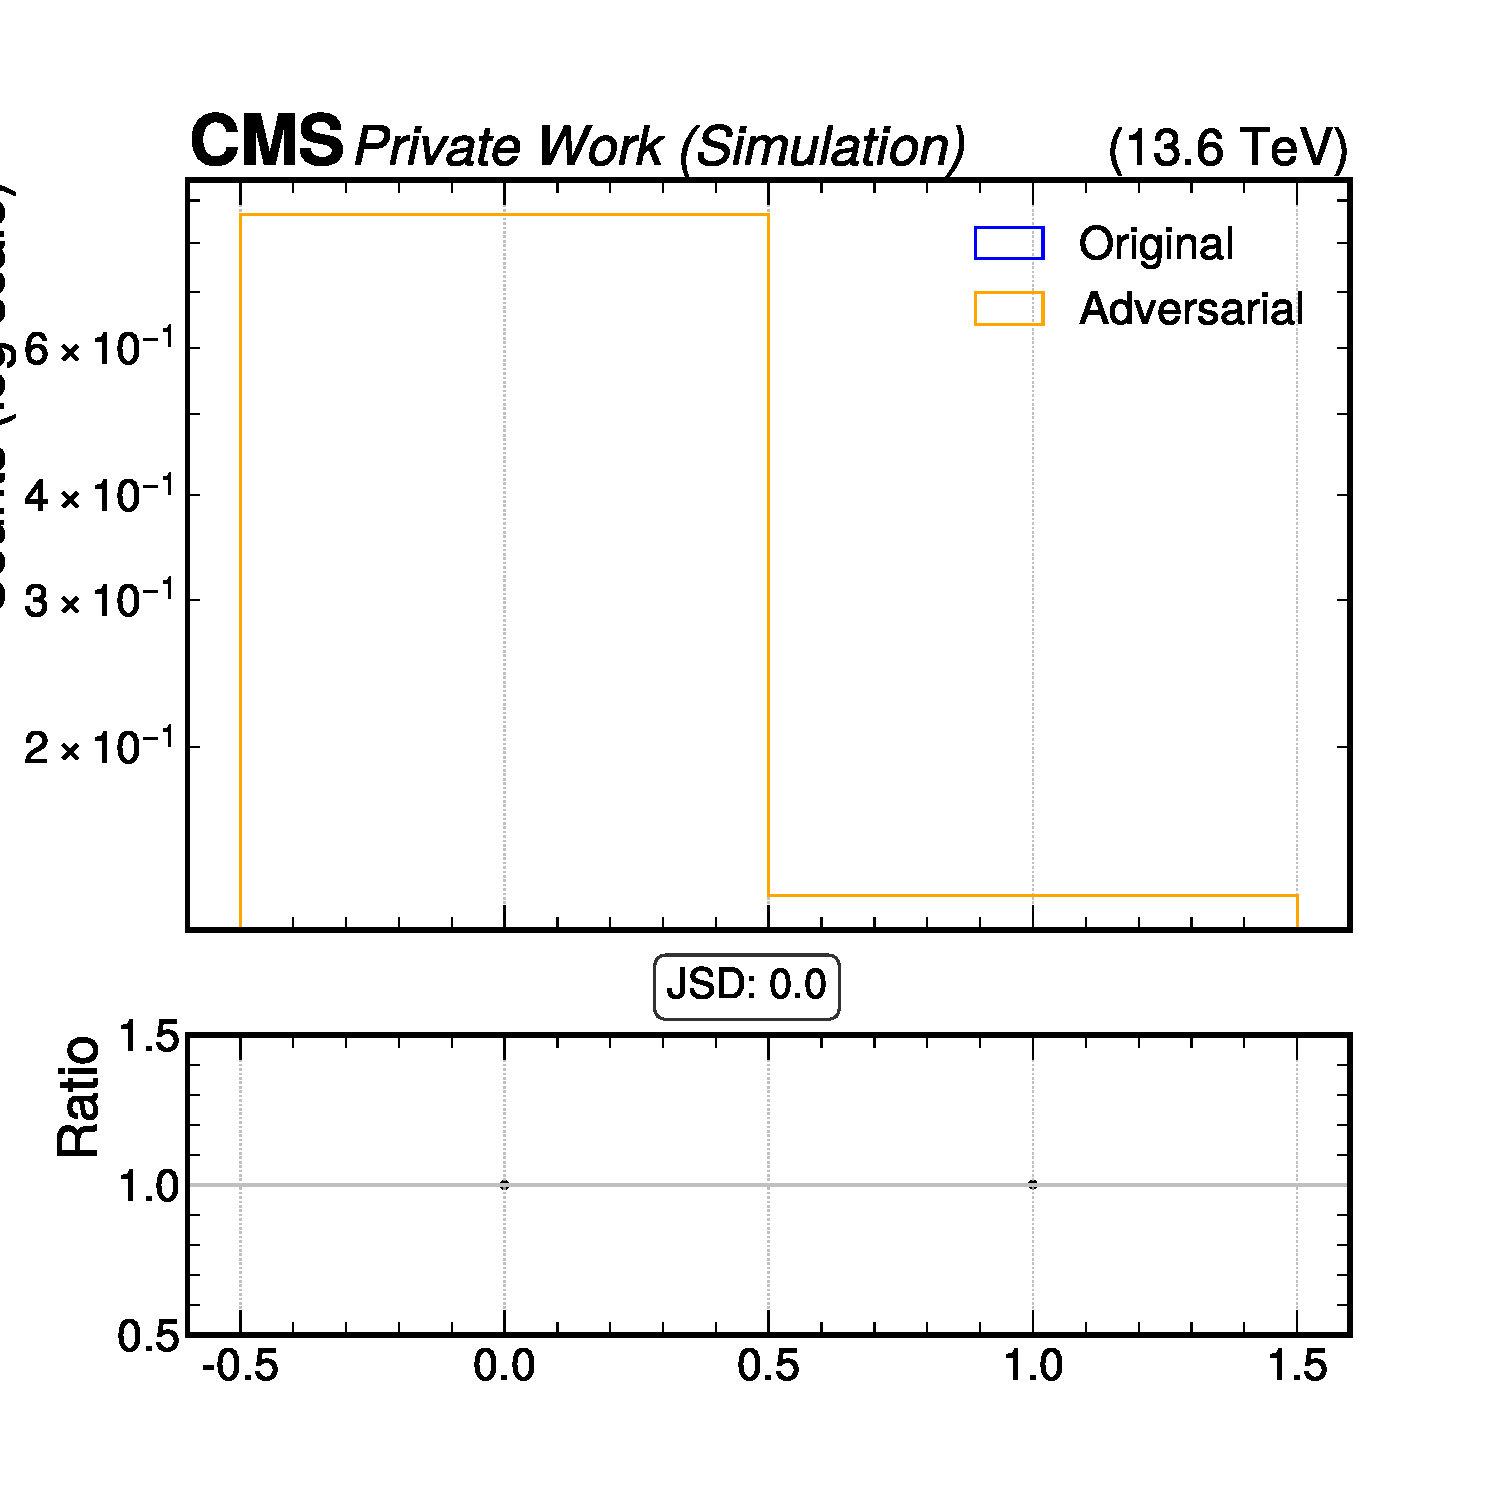
\includegraphics[width=\linewidth]{media/output/features/compare/intprob_2/cmp_npf_arr_Npfcan_isGamma.pdf}
    \caption{Input similarity for PIP(2).}
  \end{subfigure}\hfill
  \begin{subfigure}[t]{0.32\textwidth}
    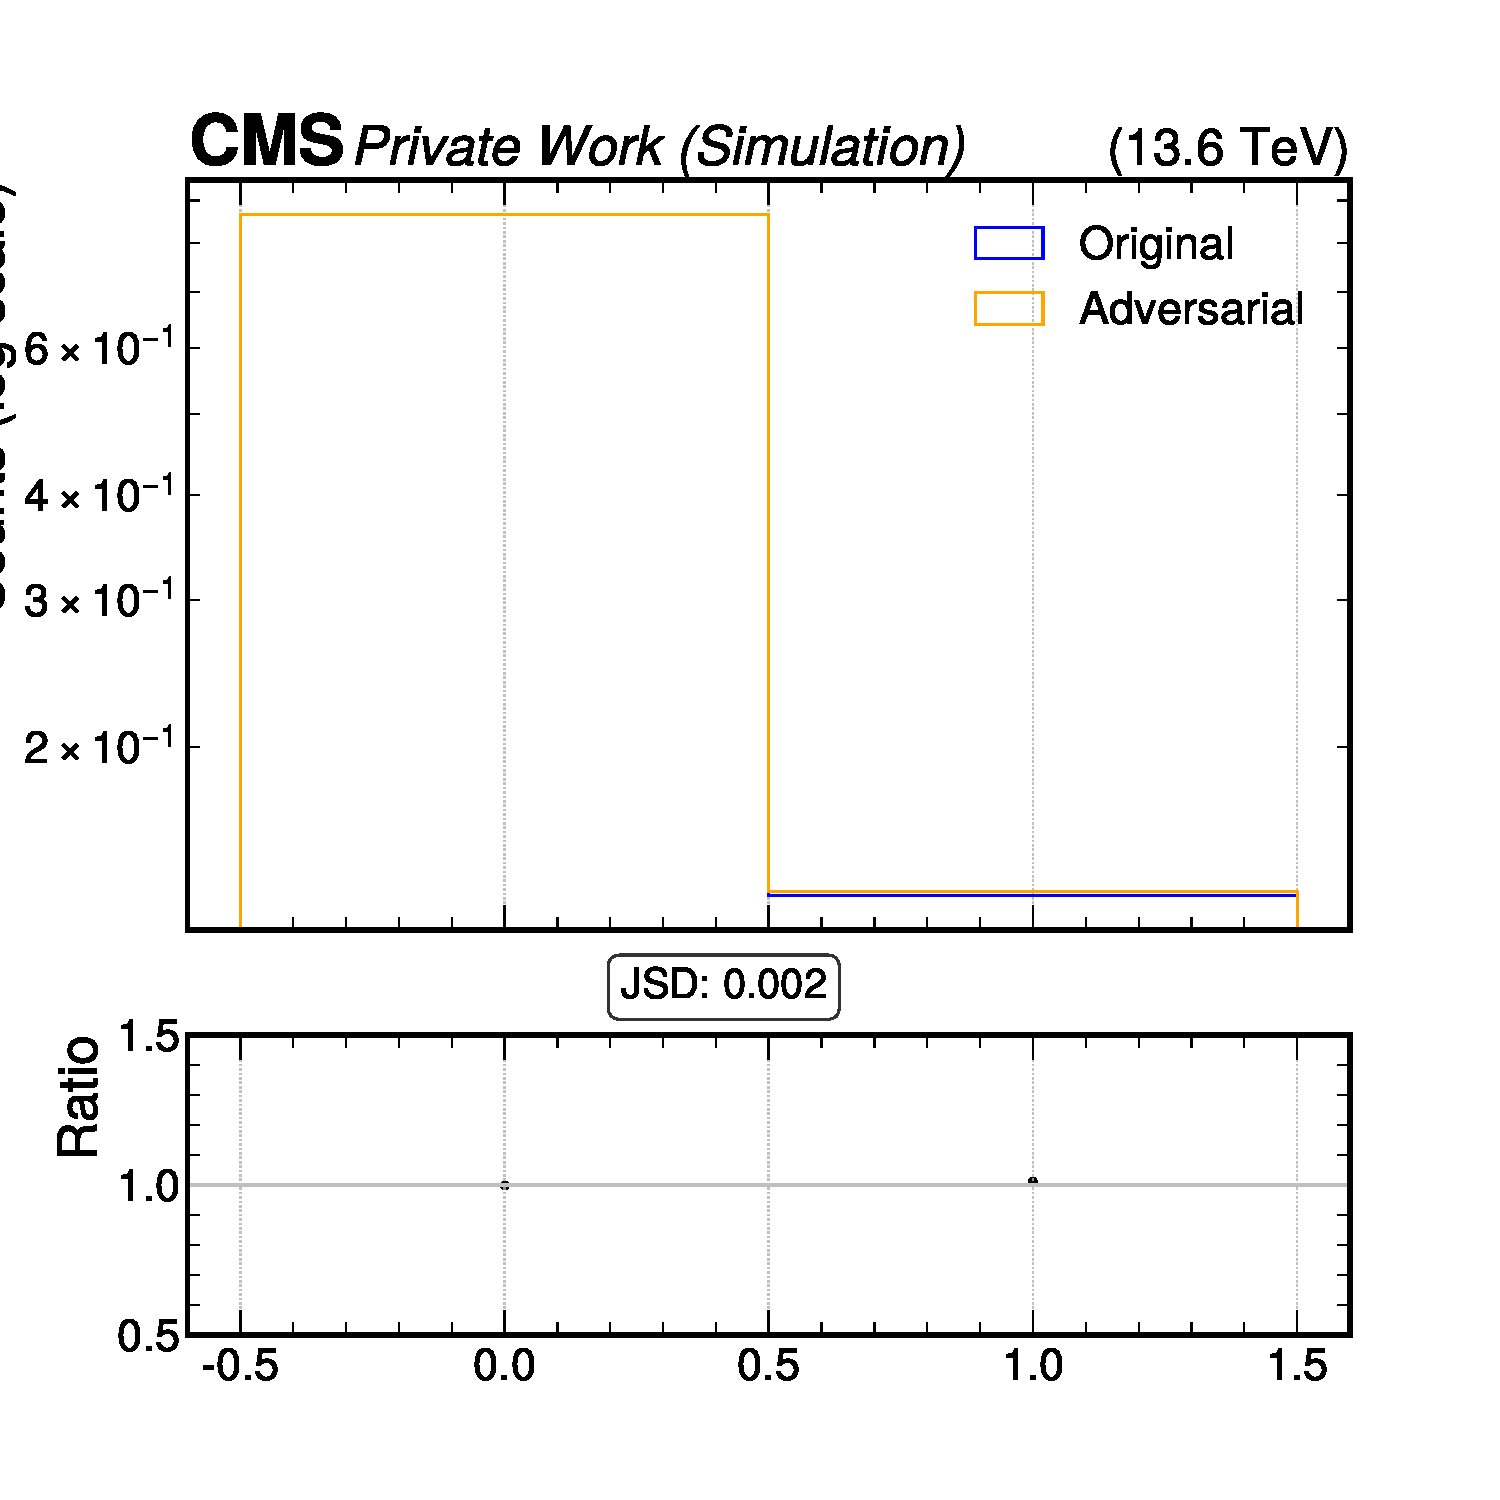
\includegraphics[width=\linewidth]{media/output/features/compare/intprob_3/cmp_npf_arr_Npfcan_isGamma.pdf}
    \caption{Input similarity for PIP(3).}
  \end{subfigure}

  \caption{Histogram of \texttt{Npfcan\_isGamma} for multiple iterations of PIP tested against nominal inputs.}
  \label{fig:intprob_input_Npfcan_isGamma}
\end{figure}